\documentclass{report}\usepackage[]{graphicx}\usepackage[]{color}
%% maxwidth is the original width if it is less than linewidth
%% otherwise use linewidth (to make sure the graphics do not exceed the margin)
\makeatletter
\def\maxwidth{ %
  \ifdim\Gin@nat@width>\linewidth
    \linewidth
  \else
    \Gin@nat@width
  \fi
}
\makeatother

\definecolor{fgcolor}{rgb}{0.345, 0.345, 0.345}
\newcommand{\hlnum}[1]{\textcolor[rgb]{0.686,0.059,0.569}{#1}}%
\newcommand{\hlstr}[1]{\textcolor[rgb]{0.192,0.494,0.8}{#1}}%
\newcommand{\hlcom}[1]{\textcolor[rgb]{0.678,0.584,0.686}{\textit{#1}}}%
\newcommand{\hlopt}[1]{\textcolor[rgb]{0,0,0}{#1}}%
\newcommand{\hlstd}[1]{\textcolor[rgb]{0.345,0.345,0.345}{#1}}%
\newcommand{\hlkwa}[1]{\textcolor[rgb]{0.161,0.373,0.58}{\textbf{#1}}}%
\newcommand{\hlkwb}[1]{\textcolor[rgb]{0.69,0.353,0.396}{#1}}%
\newcommand{\hlkwc}[1]{\textcolor[rgb]{0.333,0.667,0.333}{#1}}%
\newcommand{\hlkwd}[1]{\textcolor[rgb]{0.737,0.353,0.396}{\textbf{#1}}}%

\usepackage{framed}
\makeatletter
\newenvironment{kframe}{%
 \def\at@end@of@kframe{}%
 \ifinner\ifhmode%
  \def\at@end@of@kframe{\end{minipage}}%
  \begin{minipage}{\columnwidth}%
 \fi\fi%
 \def\FrameCommand##1{\hskip\@totalleftmargin \hskip-\fboxsep
 \colorbox{shadecolor}{##1}\hskip-\fboxsep
     % There is no \\@totalrightmargin, so:
     \hskip-\linewidth \hskip-\@totalleftmargin \hskip\columnwidth}%
 \MakeFramed {\advance\hsize-\width
   \@totalleftmargin\z@ \linewidth\hsize
   \@setminipage}}%
 {\par\unskip\endMakeFramed%
 \at@end@of@kframe}
\makeatother

\definecolor{shadecolor}{rgb}{.97, .97, .97}
\definecolor{messagecolor}{rgb}{0, 0, 0}
\definecolor{warningcolor}{rgb}{1, 0, 1}
\definecolor{errorcolor}{rgb}{1, 0, 0}
\newenvironment{knitrout}{}{} % an empty environment to be redefined in TeX

\usepackage{alltt}

\usepackage[margin=1in,bottom=.5in,includehead,includefoot]{geometry}
\usepackage{hyperref}
\usepackage{alltt}
\usepackage{fancyhdr}
\pagestyle{fancy}
\usepackage{minitoc}
\fancyhf{}
 
%comment these lines out to revert to default font
\usepackage{kpfonts}
\usepackage[T1]{fontenc}
\usepackage{inconsolata}
\IfFileExists{upquote.sty}{\usepackage{upquote}}{}
\begin{document}

\minitoc

\begin{titlepage}
    \begin{center}
        \vspace*{1cm}
        
        \textbf{An Introductory Text on Using R As a Statistical Computing Software}
        
        \vspace{0.5cm}
        For Use in the Biomedical and Life Sciences 
        
        \vspace{1.5cm}
        
        \textbf{Morgan F. Breitmeyer}
        
        \vfill
        
        
        \vspace{0.8cm}
        
        %\includegraphics[width=0.4\textwidth]{university}
        
        Harvard University\\
        Cambridge, MA\\
        \today
        
    \end{center}
\end{titlepage}

%% WRITE A PREFACE 
%JV: Will eventually need a longer introduction with some details about downloading R, R Studio, etc. Also clarify the relationship between what OI Biostat shows vs. this book (e.g., difference between figures)

\setcounter{tocdepth}{1}
\dominitoc
\tableofcontents

\newpage 
\setcounter{chapter}{-1}
\chapter{Preface}
\minitoc

This text is a companion to \textit{Introductory Statistics for the Life and Biomedical Sciences}; while the main text focuses on statistical concepts and ideas, this supplement provides details about how to use the statistical computing language \textsf{R}.

This is a preview text so this package is not available just yet, but when it is available, all of the necessary data will be accessible using the following commands.  
%' % All the datasets used in the text can be accessed by downloading the OIBiostat package from \textsf{R}. Run the following command to download the package:
%' 
%' %% These commands aren't going to work until we have uploaded the package to CRAN. Just skip it for now and require below.
\begin{knitrout}
\definecolor{shadecolor}{rgb}{0.969, 0.969, 0.969}\color{fgcolor}\begin{kframe}
\begin{alltt}
\hlkwd{install.packages}\hlstd{(}\hlstr{"OIBioStat"}\hlstd{)}  \hlcom{## make sure to include the quotations}
\end{alltt}
\end{kframe}
\end{knitrout}
%' 
%' The above command only needs to be run once. Each time a dataset in the package is needed, run the following command: 
%' 
\begin{knitrout}
\definecolor{shadecolor}{rgb}{0.969, 0.969, 0.969}\color{fgcolor}\begin{kframe}
\begin{alltt}
\hlkwd{require}\hlstd{(OIBioStat)} \hlcom{## note the lack of quotations here}
\end{alltt}
\end{kframe}
\end{knitrout}

\newpage 
\chapter{Introduction to Basic Techniques}
\minitoc

\vspace{0.5cm} 

This chapter introduces basic commands for manipulating datasets, including how to calculate numerical summaries, create tables from data, and make graphical plots. 

\section{Case study: preventing peanut allergies}

The \texttt{LEAP} dataset contains the results of the "Learning Early About Peanut Allergy" (LEAP) study, an experiment conducted to assess whether early exposure to peanut products reduces the probability of peanut allergies developing. To access the documentation associated with the dataset, run the following command: 

\begin{knitrout}
\definecolor{shadecolor}{rgb}{0.969, 0.969, 0.969}\color{fgcolor}\begin{kframe}
\begin{alltt}
\hlkwd{help}\hlstd{(LEAP)}
\end{alltt}
\end{kframe}
\end{knitrout}

A file will appear in the Help pane that provides some basic information about the dataset:

\begin{itemize}
\item \textbf{Description:} A general overview of the dataset. 
\item \textbf{Usage:} Instructions for how to load the dataset. 
\item \textbf{Format:} The names and descriptions of each variable in the dataset, including information about variable type and measurement units.
\item \textbf{Details:} Additional details about the conditions under which the data were collected.
\item \textbf{Source}: Information about where the data originates from.
\end{itemize}

To view the dataset itself, run:

\begin{knitrout}
\definecolor{shadecolor}{rgb}{0.969, 0.969, 0.969}\color{fgcolor}\begin{kframe}
\begin{alltt}
\hlkwd{View}\hlstd{(LEAP)}
\end{alltt}
\end{kframe}
\end{knitrout}

In the main console pane, a window will appear that shows the entire dataset. The variable names are displayed across the top, as the names of the columns. Data for each case in the study are contained within the rows. Note that the farthest left column shows the \textbf{indices}, which are computer-generated values that allow specific rows in the dataset to be accessed. These can be used to view a specific portion of the data.

For example, to print out data contained in the first 5 rows and first 3 columns of the data, use the following syntax:

\begin{knitrout}
\definecolor{shadecolor}{rgb}{0.969, 0.969, 0.969}\color{fgcolor}\begin{kframe}
\begin{alltt}
\hlstd{LEAP[}\hlnum{1}\hlopt{:}\hlnum{5}\hlstd{,}\hlnum{1}\hlopt{:}\hlnum{3}\hlstd{]}
\end{alltt}
\begin{verbatim}
##   participant.ID    treatment.group age.months
## 1    LEAP_100522 Peanut Consumption     6.0780
## 2    LEAP_103358 Peanut Consumption     7.5893
## 3    LEAP_105069   Peanut Avoidance     5.9795
## 4    LEAP_105328 Peanut Consumption     7.0308
## 5    LEAP_106377   Peanut Avoidance     6.4066
\end{verbatim}
\end{kframe}
\end{knitrout}

The bracket notation after the dataset name implies location; the syntax \texttt{dataset[rows,columns]} specifies rows 1 through 5 and columns 1 through 6. To access only the first 5 rows, but all the columns, leave an empty space where the columns would usually be specified:

\begin{knitrout}
\definecolor{shadecolor}{rgb}{0.969, 0.969, 0.969}\color{fgcolor}\begin{kframe}
\begin{alltt}
\hlcom{## note the space (or lack of text after the comma)}
\hlstd{LEAP[}\hlnum{1}\hlopt{:}\hlnum{5}\hlstd{, ]}
\end{alltt}
\begin{verbatim}
##   participant.ID    treatment.group age.months    sex primary.ethnicity
## 1    LEAP_100522 Peanut Consumption     6.0780 Female             Black
## 2    LEAP_103358 Peanut Consumption     7.5893 Female             White
## 3    LEAP_105069   Peanut Avoidance     5.9795   Male             White
## 4    LEAP_105328 Peanut Consumption     7.0308 Female             White
## 5    LEAP_106377   Peanut Avoidance     6.4066   Male             White
##   overall.V60.outcome
## 1            PASS OFC
## 2            PASS OFC
## 3            PASS OFC
## 4            PASS OFC
## 5            PASS OFC
\end{verbatim}
\end{kframe}
\end{knitrout}

Alternatively, since there are 6 columns in the dataset, the command \texttt{LEAP[1:5,1:6]} would also achieve the same result. This is a common theme in \textsf{R} -- there can be several ways to accomplish a desired result. 

\textit{OI Biostat} Table 1.1 shows the participant ID, treatment group, and overall outcome for five patients. It is not specified in the main text, but the data are specifically from rows 1, 2, 3, 529, and 530. The command \texttt{c()} can be used to bind the row numbers into a list, as well as to create a list of the desired columns. Columns can be referred to by name, instead of by number:

\begin{knitrout}
\definecolor{shadecolor}{rgb}{0.969, 0.969, 0.969}\color{fgcolor}\begin{kframe}
\begin{alltt}
\hlcom{## OI Biostat Table 1.1}
\hlstd{LEAP[}\hlkwd{c}\hlstd{(}\hlnum{1}\hlstd{,} \hlnum{2}\hlstd{,} \hlnum{3}\hlstd{,} \hlnum{529}\hlstd{,} \hlnum{530}\hlstd{),}\hlkwd{c}\hlstd{(}\hlstr{"participant.ID"}\hlstd{,} \hlstr{"treatment.group"}\hlstd{,}
                         \hlstr{"overall.V60.outcome"}\hlstd{)]}
\end{alltt}
\begin{verbatim}
##     participant.ID    treatment.group overall.V60.outcome
## 1      LEAP_100522 Peanut Consumption            PASS OFC
## 2      LEAP_103358 Peanut Consumption            PASS OFC
## 3      LEAP_105069   Peanut Avoidance            PASS OFC
## 639    LEAP_994047   Peanut Avoidance            PASS OFC
## 640    LEAP_997608 Peanut Consumption            PASS OFC
\end{verbatim}
\end{kframe}
\end{knitrout}

Two-way summary tables organize the data according to two variables and display the number of counts matching each combination of variable categories. The following code corresponds to \textit{OI~Biostat} Table~1.2, which groups participants into categories based on treatment group and overall outcome. In the \texttt{table()} command, the first variable specifies the rows and the second variable specifies the columns. The addition of the \texttt{addmargins()} command prints the sums of the rows and columns on the sides of the table.

\begin{knitrout}
\definecolor{shadecolor}{rgb}{0.969, 0.969, 0.969}\color{fgcolor}\begin{kframe}
\begin{alltt}
\hlcom{## Table 1.2}
\hlkwd{table}\hlstd{(LEAP}\hlopt{$}\hlstd{treatment.group, LEAP}\hlopt{$}\hlstd{overall.V60.outcome)}
\end{alltt}
\begin{verbatim}
##                     
##                      FAIL OFC PASS OFC
##   Peanut Avoidance         36      227
##   Peanut Consumption        5      262
\end{verbatim}
\begin{alltt}
\hlkwd{addmargins}\hlstd{(}\hlkwd{table}\hlstd{(LEAP}\hlopt{$}\hlstd{treatment.group, LEAP}\hlopt{$}\hlstd{overall.V60.outcome))}
\end{alltt}
\begin{verbatim}
##                     
##                      FAIL OFC PASS OFC Sum
##   Peanut Avoidance         36      227 263
##   Peanut Consumption        5      262 267
##   Sum                      41      489 530
\end{verbatim}
\end{kframe}
\end{knitrout}


\section{Data Basics}

Entire datasets can be partitioned into data frames using bracket notation. For example, \textit{OI Biostat} Table 1.3 shows a data frame consisting of rows 1-3 and 150 (and all columns) from the \texttt{frog.altitude} dataset. The data frame can then be given a specific name, such as \texttt{frog.df}, and directly called on for later operations.

%%JV: order of variables should be the same between companion and oi biostat

\begin{knitrout}
\definecolor{shadecolor}{rgb}{0.969, 0.969, 0.969}\color{fgcolor}\begin{kframe}
\begin{alltt}
\hlcom{## Table 1.3}
\hlstd{frog.df} \hlkwb{=} \hlstd{frog.altitude.data[}\hlkwd{c}\hlstd{(}\hlnum{1}\hlopt{:}\hlnum{3}\hlstd{,} \hlnum{150}\hlstd{),]}
\hlstd{frog.df}
\end{alltt}
\begin{verbatim}
##     altitude latitude clutch.size body.size clutch.volume egg.size
## 1   3,462.00    34.82    181.9701  3.630781      177.8279 1.949845
## 2   3,462.00    34.82    269.1535  3.630781      257.0396 1.949845
## 3   3,462.00    34.82    158.4893  3.715352      151.3561 1.949845
## 150 2,597.00    34.05    537.0318        NA      776.2471 2.238721
\end{verbatim}
\end{kframe}
\end{knitrout}

Similarly, matrix notation can be used to create \textit{OI Biostat} Table 1.5.

\begin{knitrout}
\definecolor{shadecolor}{rgb}{0.969, 0.969, 0.969}\color{fgcolor}\begin{kframe}
\begin{alltt}
\hlcom{## Table 1.5}
\hlstd{famuss[}\hlkwd{c}\hlstd{(}\hlnum{1}\hlstd{,}\hlnum{2}\hlstd{,}\hlnum{3}\hlstd{,}\hlnum{595}\hlstd{),}\hlkwd{c}\hlstd{(} \hlstr{"sex"}\hlstd{,} \hlstr{"age"}\hlstd{,} \hlstr{"race"}\hlstd{,} \hlstr{"height"}\hlstd{,} \hlstr{"weight"}\hlstd{,} \hlstr{"actn3.r577x"}\hlstd{,}
                       \hlstr{"ndrm.ch"}\hlstd{)]}
\end{alltt}
\begin{verbatim}
##         sex age      race height weight actn3.r577x ndrm.ch
## 1    Female  27 Caucasian   65.0    199          CC    40.0
## 2      Male  36 Caucasian   71.7    189          CT    25.0
## 3    Female  24 Caucasian   65.0    134          CT    40.0
## 1348 Female  30 Caucasian   64.0    134          CC    43.8
\end{verbatim}
\end{kframe}
\end{knitrout}

\stepcounter{section}
\section{Numerical Data}

Numerical summaries can be quickly and easily calculated using \textsf{R}. The \texttt{summary()} command is one way to access several numerical summaries at once, including the minimum and maximum values of a variable:
\begin{knitrout}
\definecolor{shadecolor}{rgb}{0.969, 0.969, 0.969}\color{fgcolor}\begin{kframe}
\begin{alltt}
\hlkwd{summary}\hlstd{(frog.altitude.data}\hlopt{$}\hlstd{clutch.volume)}
\end{alltt}
\begin{verbatim}
##    Min. 1st Qu.  Median    Mean 3rd Qu.    Max. 
##   151.4   609.6   831.8   882.5  1096.0  2630.0
\end{verbatim}
\end{kframe}
\end{knitrout}

\subsection{Measures of center: mean and median}

The \textbf{mean} of a numerical value is the sum of all observations divided by the number of observations, where $x_1, x_2, \dots, x_n$ represent the $n$ observed values:

\begin{align*}
		\overline{x} = \frac{x_1+x_2+\cdots+x_n}{n}
\end{align*}

This calculation can be completed in \textsf{R} the same way as a hand calculation is done:
\begin{knitrout}
\definecolor{shadecolor}{rgb}{0.969, 0.969, 0.969}\color{fgcolor}\begin{kframe}
\begin{alltt}
\hlcom{# identify n, the number of observations in the data}
\hlstd{n} \hlkwb{=} \hlkwd{length}\hlstd{(frog.altitude.data}\hlopt{$}\hlstd{clutch.volume)}
\hlstd{n}
\end{alltt}
\begin{verbatim}
## [1] 431
\end{verbatim}
\begin{alltt}
\hlcom{# calculate the sum of all observations and divide by n}
\hlkwd{sum}\hlstd{(frog.altitude.data}\hlopt{$}\hlstd{clutch.volume)}\hlopt{/}\hlstd{n}
\end{alltt}
\begin{verbatim}
## [1] 882.474
\end{verbatim}
\end{kframe}
\end{knitrout}

Alternatively, the \textsf{R} function \texttt{mean()} can be directly applied to the variable of interest:
\begin{knitrout}
\definecolor{shadecolor}{rgb}{0.969, 0.969, 0.969}\color{fgcolor}\begin{kframe}
\begin{alltt}
\hlstd{x.bar} \hlkwb{=} \hlkwd{mean}\hlstd{(frog.altitude.data}\hlopt{$}\hlstd{clutch.volume)}
\hlstd{x.bar}
\end{alltt}
\begin{verbatim}
## [1] 882.474
\end{verbatim}
\begin{alltt}
\hlcom{## round to the first decimal}
\hlkwd{round}\hlstd{(x.bar,} \hlnum{1}\hlstd{)}
\end{alltt}
\begin{verbatim}
## [1] 882.5
\end{verbatim}
\end{kframe}
\end{knitrout}

To identify the \textbf{median} value, use the following command:

\begin{knitrout}
\definecolor{shadecolor}{rgb}{0.969, 0.969, 0.969}\color{fgcolor}\begin{kframe}
\begin{alltt}
\hlkwd{median}\hlstd{(frog.altitude.data}\hlopt{$}\hlstd{clutch.volume)}
\end{alltt}
\begin{verbatim}
## [1] 831.7638
\end{verbatim}
\end{kframe}
\end{knitrout}

\subsection{Measures of spread: standard deviation and variance}

The distance of a single observation from the mean is its \textbf{deviation}. The following command produces the deviations for the $1^{st}$, $2^{nd}$, $3^{rd}$, and $431^{th}$ observations in the \texttt{clutch.volume} variable.

\begin{knitrout}
\definecolor{shadecolor}{rgb}{0.969, 0.969, 0.969}\color{fgcolor}\begin{kframe}
\begin{alltt}
\hlstd{frog.altitude.data}\hlopt{$}\hlstd{clutch.volume[}\hlkwd{c}\hlstd{(}\hlnum{1}\hlstd{,}\hlnum{2}\hlstd{,}\hlnum{3}\hlstd{,}\hlnum{431}\hlstd{)]}\hlopt{-}\hlstd{x.bar}
\end{alltt}
\begin{verbatim}
## [1] -704.64604 -625.43440 -731.11786   50.78032
\end{verbatim}
\end{kframe}
\end{knitrout}

The sample \textbf{standard deviation} is computed as the square root of the \textbf{variance}, which is the sum of squared deviations divided by the number of observations minus 1. 

\begin{align*}
		s = \sqrt{\frac{({x_1 - \overline{x})}^{2}+({x_2 - \overline{x})}^{2}+\cdots+({x_n - \overline{x})}^{2}}{n-1}}
\end{align*}

The following steps illustrate how to calculate the variance and standard deviation using the formula: 

\begin{knitrout}
\definecolor{shadecolor}{rgb}{0.969, 0.969, 0.969}\color{fgcolor}\begin{kframe}
\begin{alltt}
\hlcom{# calculate all deviations}
\hlstd{dev} \hlkwb{=} \hlstd{frog.altitude.data}\hlopt{$}\hlstd{clutch.volume} \hlopt{-} \hlstd{x.bar}

\hlcom{# sum the squares of the deviations and divide by n - 1}
\hlstd{var} \hlkwb{=} \hlstd{(}\hlkwd{sum}\hlstd{(dev}\hlopt{^}\hlnum{2}\hlstd{))}\hlopt{/}\hlstd{(n}\hlopt{-}\hlnum{1}\hlstd{)}
\hlstd{var}
\end{alltt}
\begin{verbatim}
## [1] 143680.9
\end{verbatim}
\begin{alltt}
\hlcom{# take the square root of the variance}
\hlstd{sd} \hlkwb{=} \hlkwd{sqrt}\hlstd{(var)}
\hlstd{sd}
\end{alltt}
\begin{verbatim}
## [1] 379.0527
\end{verbatim}
\end{kframe}
\end{knitrout}

Alternatively, use the \textsf{R} functions \texttt{var()} and \texttt{sd()}:

\begin{knitrout}
\definecolor{shadecolor}{rgb}{0.969, 0.969, 0.969}\color{fgcolor}\begin{kframe}
\begin{alltt}
\hlkwd{var}\hlstd{(frog.altitude.data}\hlopt{$}\hlstd{clutch.volume)}
\end{alltt}
\begin{verbatim}
## [1] 143680.9
\end{verbatim}
\begin{alltt}
\hlkwd{sd}\hlstd{(frog.altitude.data}\hlopt{$}\hlstd{clutch.volume)}
\end{alltt}
\begin{verbatim}
## [1] 379.0527
\end{verbatim}
\end{kframe}
\end{knitrout}

Variability can also be measured using the \textbf{interquartile range (IQR)}, which equals the third quartile (the $75^{th}$ percentile) minus the first quartile (the $25^{th}$ percentile). 

\begin{knitrout}
\definecolor{shadecolor}{rgb}{0.969, 0.969, 0.969}\color{fgcolor}\begin{kframe}
\begin{alltt}
\hlkwd{IQR}\hlstd{(frog.altitude.data}\hlopt{$}\hlstd{clutch.volume)}
\end{alltt}
\begin{verbatim}
## [1] 486.9009
\end{verbatim}
\end{kframe}
\end{knitrout}

\subsection{Robust statistics}

In the \texttt{frog.altitude} dataset, there are four extreme values for clutch volume that are larger than 2,000 mm$^3$. To illustrate how the summary statistics are influenced by extreme values, \textit{OI Biostat} Table 1.15 shows summary statistics for the data without the four largest observations. 

The subset of the data with values less than 2,000 mm$^3$ can be pulled out by first specifying a logical condition, which assigns \texttt{TRUE} or \texttt{FALSE} to each entry. 

\begin{knitrout}
\definecolor{shadecolor}{rgb}{0.969, 0.969, 0.969}\color{fgcolor}\begin{kframe}
\begin{alltt}
\hlcom{# logical condition}
\hlstd{less.than.2000} \hlkwb{=} \hlstd{frog.altitude.data}\hlopt{$}\hlstd{clutch.volume}\hlopt{<=} \hlnum{2000}

\hlcom{# view the first 5 values}
\hlstd{less.than.2000[}\hlnum{1}\hlopt{:}\hlnum{5}\hlstd{]}
\end{alltt}
\begin{verbatim}
## [1] TRUE TRUE TRUE TRUE TRUE
\end{verbatim}
\end{kframe}
\end{knitrout}

Bracket notation can then be used to calculate summary statistics specifically for the values in \texttt{clutch.volume} that satisfy the logical condition.

\begin{knitrout}
\definecolor{shadecolor}{rgb}{0.969, 0.969, 0.969}\color{fgcolor}\begin{kframe}
\begin{alltt}
\hlcom{## robust estimates}
\hlkwd{median}\hlstd{(frog.altitude.data}\hlopt{$}\hlstd{clutch.volume[less.than.2000])}
\end{alltt}
\begin{verbatim}
## [1] 831.7638
\end{verbatim}
\begin{alltt}
\hlkwd{IQR}\hlstd{(frog.altitude.data}\hlopt{$}\hlstd{clutch.volume[less.than.2000])}
\end{alltt}
\begin{verbatim}
## [1] 493.9186
\end{verbatim}
\begin{alltt}
\hlcom{## non-robust estimates}
\hlkwd{mean}\hlstd{(frog.altitude.data}\hlopt{$}\hlstd{clutch.volume[less.than.2000])}
\end{alltt}
\begin{verbatim}
## [1] 867.9425
\end{verbatim}
\begin{alltt}
\hlkwd{sd}\hlstd{(frog.altitude.data}\hlopt{$}\hlstd{clutch.volume[less.than.2000])}
\end{alltt}
\begin{verbatim}
## [1] 349.1596
\end{verbatim}
\end{kframe}
\end{knitrout}

\subsection{Visualizing distributions of data}
While most numerical summaries can be calculated by hand, \textsf{R} is essential for creating graphical summaries.

\subsubsection{Histograms}
A \textbf{histogram} provides a view of data density. Observations are sorted into different bins based on their value, and the histogram shows the number of observations in each bin. The following command produces a histogram of the \texttt{clutch.volume} variable.

\begin{knitrout}
\definecolor{shadecolor}{rgb}{0.969, 0.969, 0.969}\color{fgcolor}\begin{kframe}
\begin{alltt}
\hlkwd{hist}\hlstd{(frog.altitude.data}\hlopt{$}\hlstd{clutch.volume)}
\end{alltt}
\end{kframe}
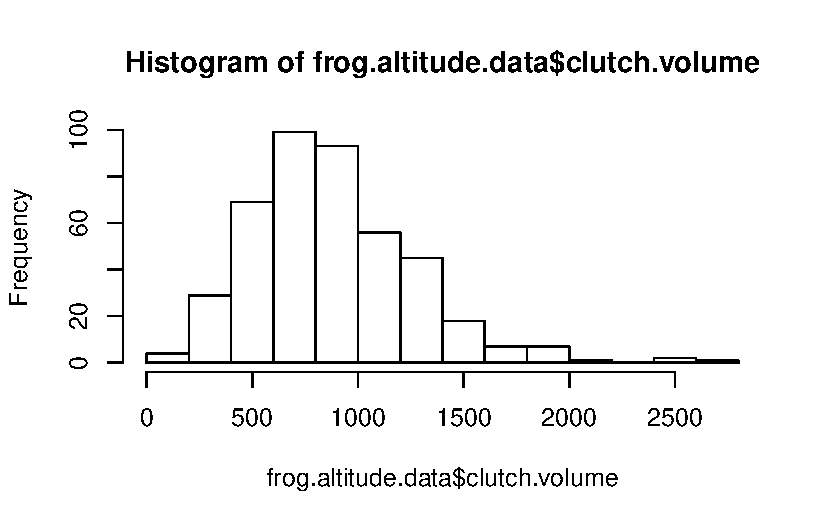
\includegraphics[width=\maxwidth]{figure/unnamed-chunk-19-1} 

\end{knitrout}

The \texttt{hist()} function takes several arguments:
\begin{itemize}
\item \texttt{x}: variable of interest
\item \texttt{breaks}: number of bins
\item \texttt{col}: color of the bars, enclosed in \texttt{""}
\item \texttt{xlab}: $x$-axis label, enclosed in \texttt{""}
\item \texttt{ylab}: $y$-axis label, enclosed in \texttt{""}
\item \texttt{xlim}: range of values for the $x$-axis, in the form \texttt{c(lower bound, upper bound)}
\item \texttt{ylim}: range of values for the $y$-axis, in the form \texttt{c(lower bound, upper bound)}
\item \texttt{main}: main title of the plot, enclosed in \texttt{""} 
\item \texttt{plot}: if \texttt{TRUE} (default), a histogram is plotted; otherwise, data about the histogram is returned
\end{itemize}

As seen above, not all arguments must be specified; only the \texttt{x} argument is necessary. When options are not specified, \textsf{R} uses the default options, such as the default color of white for the histogram bars.

The following command reproduces \textit{OI Biostat} Table 1.16 and Figure 1.17.

\begin{knitrout}
\definecolor{shadecolor}{rgb}{0.969, 0.969, 0.969}\color{fgcolor}\begin{kframe}
\begin{alltt}
\hlcom{## Table 1.16}
\hlkwd{hist}\hlstd{(frog.altitude.data}\hlopt{$}\hlstd{clutch.volume,} \hlkwc{breaks} \hlstd{=} \hlnum{14}\hlstd{,} \hlkwc{plot} \hlstd{=} \hlnum{FALSE}\hlstd{)}\hlopt{$}\hlstd{counts}
\end{alltt}
\begin{verbatim}
##  [1]  4 29 69 99 93 56 45 18  7  7  1  0  2  1
\end{verbatim}
\begin{alltt}
\hlcom{## Figure 1.17}
\hlkwd{hist}\hlstd{(}\hlkwc{x} \hlstd{= frog.altitude.data}\hlopt{$}\hlstd{clutch.volume,} \hlkwc{breaks} \hlstd{=} \hlnum{14}\hlstd{,} \hlkwc{col} \hlstd{=} \hlstr{"dodgerblue"}\hlstd{,}
     \hlkwc{xlab} \hlstd{=} \hlstr{"Clutch Volume"}\hlstd{,} \hlkwc{ylab} \hlstd{=} \hlstr{"Frequency"}\hlstd{,} \hlkwc{ylim} \hlstd{=} \hlkwd{c}\hlstd{(}\hlnum{0}\hlstd{,} \hlnum{100}\hlstd{),}
     \hlkwc{main} \hlstd{=} \hlstr{"Histogram of Clutch Volume Frequencies"}\hlstd{)}
\end{alltt}
\end{kframe}
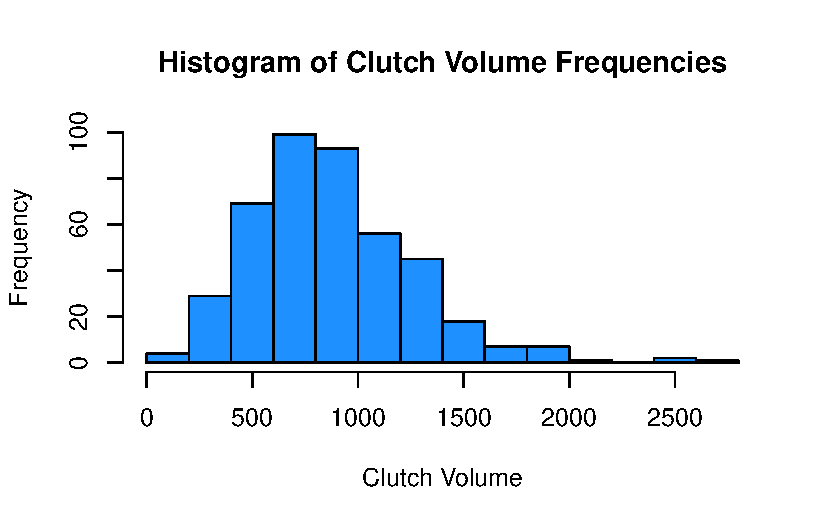
\includegraphics[width=\maxwidth]{figure/unnamed-chunk-20-1} 

\end{knitrout}


\subsubsection{Boxplots}

A \textbf{boxplot} uses five statistics to summarize a dataset, in addition to showing unusual observations. The following command produces a boxplot of the \texttt{clutch.volume} variable.

\begin{centering}
\begin{knitrout}
\definecolor{shadecolor}{rgb}{0.969, 0.969, 0.969}\color{fgcolor}\begin{kframe}
\begin{alltt}
\hlkwd{boxplot}\hlstd{(frog.altitude.data}\hlopt{$}\hlstd{clutch.volume)}
\end{alltt}
\end{kframe}
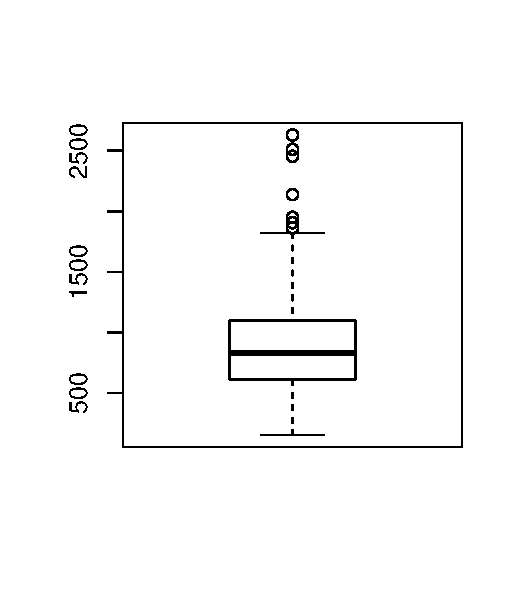
\includegraphics[width=\maxwidth]{figure/unnamed-chunk-21-1} 

\end{knitrout}
\end{centering}

Like the \texttt{hist()} function, the \texttt{boxplot()} function also takes several arguments that allow for certain parameters to be specified:
\begin{itemize}
\item \texttt{x}: variable of interest
\item \texttt{axes}: if \texttt{TRUE}, numbers are shown on the axes
\item \texttt{col}: color of the boxplot, enclosed in \texttt{""}
\item \texttt{xlab}: $x$-axis label, enclosed in \texttt{""}
\item \texttt{ylab}: $y$-axis label, enclosed in \texttt{""}
\item \texttt{xlim}: range of values for the $x$-axis, in the form \texttt{c(lower bound, upper bound)}
\item \texttt{ylim}: range of values for the $y$-axis, in the form \texttt{c(lower bound, upper bound)}
\item \texttt{main}: main title of the plot, enclosed in \texttt{""} 
\end{itemize}

The following command reproduces a simplified version of \textit{OI Biostat} Figure 1.19. 

\begin{centering}
\begin{knitrout}
\definecolor{shadecolor}{rgb}{0.969, 0.969, 0.969}\color{fgcolor}\begin{kframe}
\begin{alltt}
\hlcom{## Figure 1.19}
\hlkwd{boxplot}\hlstd{(}\hlkwc{x} \hlstd{= frog.altitude.data}\hlopt{$}\hlstd{clutch.volume,} \hlkwc{ylab} \hlstd{=} \hlstr{'Clutch Volume'}\hlstd{,} \hlkwc{axes} \hlstd{=} \hlnum{TRUE}\hlstd{,}
        \hlkwc{ylim} \hlstd{=} \hlkwd{range}\hlstd{(frog.altitude.data}\hlopt{$}\hlstd{clutch.volume))}
\end{alltt}
\end{kframe}
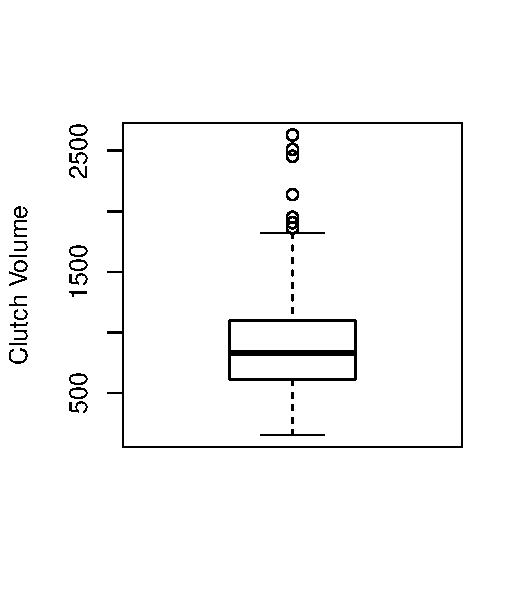
\includegraphics[width=\maxwidth]{figure/unnamed-chunk-22-1} 

\end{knitrout}
\end{centering}

\subsection{Scatterplots and correlation}
\textbf{Scatterplots} can be used to visualize the relationship between two numerical variables. In the \texttt{plot()} command, either a comma or a tilde can be used between the variable names; i.e., \texttt{plot(x,y)} versus \texttt{plot(y $\sim$ x)}.

\begin{knitrout}
\definecolor{shadecolor}{rgb}{0.969, 0.969, 0.969}\color{fgcolor}\begin{kframe}
\begin{alltt}
\hlkwd{plot}\hlstd{(frog.altitude.data}\hlopt{$}\hlstd{body.size, frog.altitude.data}\hlopt{$}\hlstd{clutch.volume)}
\end{alltt}
\end{kframe}

{\centering 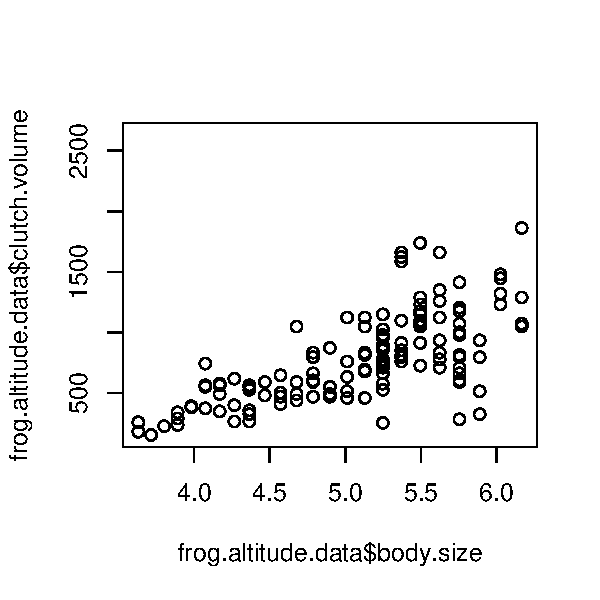
\includegraphics[width=\maxwidth]{figure/unnamed-chunk-23-1} 

}



\end{knitrout}

The \texttt{plot()} command takes the following arguments: 

\begin{itemize}
\item \texttt{x}: variable defining the $x$-coordinates 
\item \texttt{y}: variable defining the $y$-coordinates 
\item \texttt{col}: color of the dots, enclosed in \texttt{""}
\item \texttt{type}: by default, data points are marked with dots; other options include \texttt{"l"} which draws a line chart, or \texttt{"b"} which includes both dots and lines
\item \texttt{xlab}: $x$-axis label, enclosed in \texttt{""}
\item \texttt{ylab}: $y$-axis label, enclosed in \texttt{""}
\item \texttt{xlim}: range of values for the $x$-axis, in the form \texttt{c(lower bound, upper bound)}
\item \texttt{ylim}: range of values for the $y$-axis, in the form \texttt{c(lower bound, upper bound)}
\item \texttt{main}: main title of the plot, enclosed in \texttt{""} 
\end{itemize}

The \textit{plot} command has an interesting feature that you can either specify your $x$ and $y$ variables by running $plot(x,y)$ or by running $plot(y~x)$.  Either command will give the same result.  

The following command reproduces a simplified version of \textit{OI Biostat} Figure 1.20. The additional argument \texttt{pch} changes the appearance of the dots to filled dots, which is specified by \texttt{19}. 

\begin{centering}
\begin{knitrout}
\definecolor{shadecolor}{rgb}{0.969, 0.969, 0.969}\color{fgcolor}\begin{kframe}
\begin{alltt}
\hlcom{## Figure 1.20}
\hlkwd{plot}\hlstd{(frog.altitude.data}\hlopt{$}\hlstd{clutch.volume}\hlopt{~}\hlstd{frog.altitude.data}\hlopt{$}\hlstd{body.size,} \hlkwc{col} \hlstd{=} \hlstr{"dodgerblue"}\hlstd{,}
     \hlkwc{pch} \hlstd{=} \hlnum{19}\hlstd{,} \hlkwc{xlab} \hlstd{=} \hlstr{"Female Body Size (cm)"}\hlstd{,} \hlkwc{ylab} \hlstd{=} \hlkwd{expression}\hlstd{(}\hlstr{"Clutch Volume"} \hlopt{~} \hlstd{(mm}\hlopt{^}\hlnum{3}\hlstd{)))}
\end{alltt}
\end{kframe}
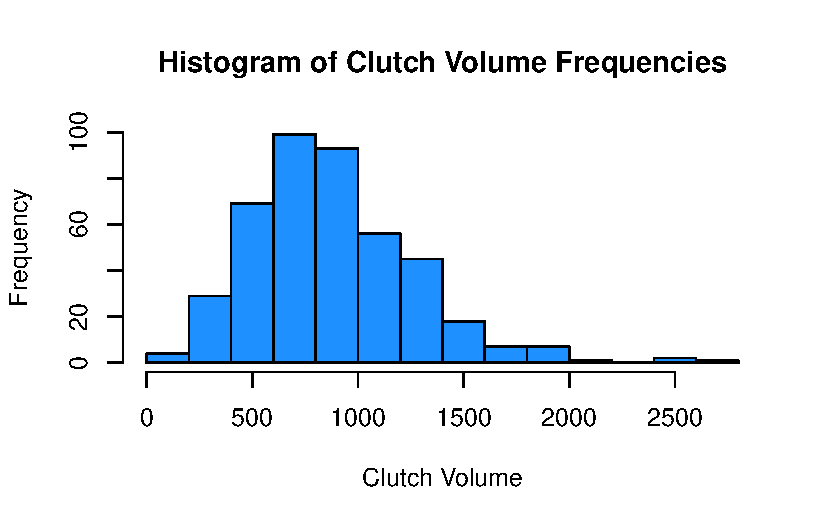
\includegraphics[width=\maxwidth]{figure/unnamed-chunk-24-1} 

\end{knitrout}
\end{centering}

Simplified versions of \textit{OI Biostat} Figures 1.21, 1.22, and 1.23 can also be reproduced using \texttt{plot()}.

\subsection{Correlation}

\textbf{Correlation} is a numerical measure of the strength of a linear relationship. The formula for correlation uses the pairing of the two variables, just as the scatterplot does in a graph, so the data used in calculating correlation is a set of $n$ ordered pairs $(x_1,y_1), (x_2,y_2), \ldots, (x_n, y_n) $.

The correlation between two variables $x$ and $y$ is given by:
		\begin{align*}
          r &=  \frac{1}{n-1}\sum^{n}_{i=1}
          \left(\frac{x_{i}-\overline{x}}
          {s_{x}}\right)\left(\frac{y_{i}-\overline{y}}{s_{y}}\right)
    \end{align*}      
where $(x_1,y_1), (x_2,y_2), \ldots, (x_n, y_n)$ are the $n$ paired values of $x$ and $y$, and $s_x$ and $s_y$ are the sample standard deviations of the $x$ and $y$ variables, respectively.     

The following illustrates the calculations for finding the correlation coefficient of (1,5), (2, 4), and (3,0), as shown in \textit{OI Biostat} Example 1.13.

\begin{knitrout}
\definecolor{shadecolor}{rgb}{0.969, 0.969, 0.969}\color{fgcolor}\begin{kframe}
\begin{alltt}
\hlcom{# define variables}
\hlstd{x} \hlkwb{=} \hlkwd{c}\hlstd{(}\hlnum{1}\hlstd{,} \hlnum{2}\hlstd{,} \hlnum{3}\hlstd{)}
\hlstd{y} \hlkwb{=} \hlkwd{c}\hlstd{(}\hlnum{5}\hlstd{,} \hlnum{4}\hlstd{,} \hlnum{0}\hlstd{)}

\hlcom{# calculate sample means}
\hlstd{x.bar} \hlkwb{=} \hlkwd{mean}\hlstd{(x)}
\hlstd{y.bar} \hlkwb{=} \hlkwd{mean}\hlstd{(y)}

\hlcom{# calculate sample sd's}
\hlstd{sd.x} \hlkwb{=} \hlkwd{sd}\hlstd{(x)}
\hlstd{sd.y} \hlkwb{=} \hlkwd{sd}\hlstd{(y)}

\hlcom{# calculate products and sum of products}
\hlstd{x.component} \hlkwb{=} \hlstd{(x} \hlopt{-} \hlstd{x.bar)}\hlopt{/}\hlstd{(sd.x)}
\hlstd{y.component} \hlkwb{=} \hlstd{(y} \hlopt{-} \hlstd{y.bar)}\hlopt{/}\hlstd{(sd.y)}
\hlstd{products} \hlkwb{=} \hlstd{x.component} \hlopt{*} \hlstd{y.component}
\hlstd{products.sum} \hlkwb{=} \hlkwd{sum}\hlstd{(products)}

\hlcom{# divide by n - 1}
\hlstd{n} \hlkwb{=} \hlkwd{length}\hlstd{(x)}   \hlcom{## n also equals length(y)}
\hlstd{r} \hlkwb{=} \hlstd{products.sum} \hlopt{/} \hlstd{(n} \hlopt{-} \hlnum{1}\hlstd{)}
\hlstd{r}
\end{alltt}
\begin{verbatim}
## [1] -0.9449112
\end{verbatim}
\end{kframe}
\end{knitrout}

It is much easier to use the \texttt{cor()} function to find correlation. 

\begin{knitrout}
\definecolor{shadecolor}{rgb}{0.969, 0.969, 0.969}\color{fgcolor}\begin{kframe}
\begin{alltt}
\hlcom{## Figure 1.22}
\hlkwd{cor}\hlstd{(x,y)}
\end{alltt}
\begin{verbatim}
## [1] -0.9449112
\end{verbatim}
\begin{alltt}
\hlkwd{plot}\hlstd{(x,y)}
\end{alltt}
\end{kframe}

{\centering 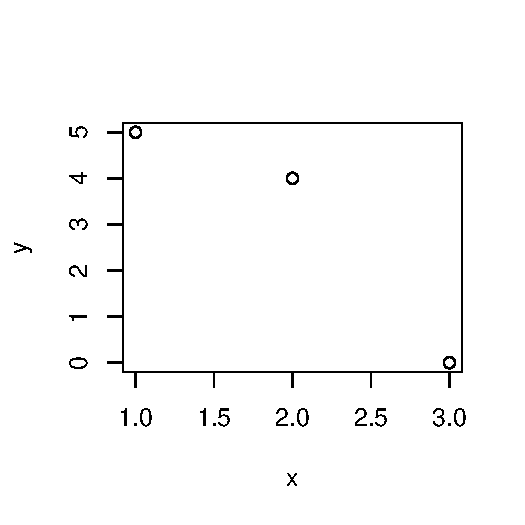
\includegraphics[width=\maxwidth]{figure/unnamed-chunk-26-1} 

}



\end{knitrout}

The correlation can also be calculated for the income versus life expectancy data plotted in \textit{OI Biostat} Figure 1.23. In this case, the command includes the argument \texttt{use = "complete.obs"} to allow for the computation to disregard any missing values in the dataset.

\begin{knitrout}
\definecolor{shadecolor}{rgb}{0.969, 0.969, 0.969}\color{fgcolor}\begin{kframe}
\begin{alltt}
\hlkwd{cor}\hlstd{(life.expectancy.income}\hlopt{$}\hlstd{income, life.expectancy.income}\hlopt{$}\hlstd{life.expectancy,}
    \hlkwc{use} \hlstd{=} \hlstr{"complete.obs"}\hlstd{)}
\end{alltt}
\begin{verbatim}
## [1] 0.6308783
\end{verbatim}
\end{kframe}
\end{knitrout}

\subsection{Transforming Data}
A \textbf{transformation} is a rescaling of data using a function. The figure below shows the original plot of income data as well as the plot of the log-transformed data. Note that the \texttt{log} command in \textsf{R} computes natural logarithms.

The function \texttt{par()} creates partitions in the graphing output. In this case, specifying \texttt{mfrow = c(1,2)} produces 1 row and 2 columns.

\begin{knitrout}
\definecolor{shadecolor}{rgb}{0.969, 0.969, 0.969}\color{fgcolor}\begin{kframe}
\begin{alltt}
\hlcom{## Figure 1.26}
\hlkwd{par}\hlstd{(}\hlkwc{mfrow} \hlstd{=} \hlkwd{c}\hlstd{(}\hlnum{1}\hlstd{,} \hlnum{2}\hlstd{))}  \hlcom{## this line allows two plots to print at the same time}
\hlkwd{hist}\hlstd{(life.expectancy.income}\hlopt{$}\hlstd{income,} \hlkwc{breaks} \hlstd{=} \hlnum{12}\hlstd{,} \hlkwc{xlab} \hlstd{=} \hlstr{"Income (USD)"}\hlstd{,}
    \hlkwc{ylab} \hlstd{=} \hlstr{"Frequency"}\hlstd{,} \hlkwc{ylim} \hlstd{=} \hlkwd{c}\hlstd{(}\hlnum{0}\hlstd{,} \hlnum{120}\hlstd{),} \hlkwc{main} \hlstd{=} \hlstr{"Untransformed"}\hlstd{)}

\hlkwd{hist}\hlstd{(}\hlkwd{log}\hlstd{(life.expectancy.income}\hlopt{$}\hlstd{income),} \hlkwc{breaks} \hlstd{=} \hlnum{12}\hlstd{,} \hlkwc{xlab} \hlstd{=} \hlstr{"Income (log USD)"}\hlstd{,}
    \hlkwc{ylab} \hlstd{=} \hlstr{"Frequency"}\hlstd{,} \hlkwc{ylim} \hlstd{=} \hlkwd{c}\hlstd{(}\hlnum{0}\hlstd{,} \hlnum{30}\hlstd{),} \hlkwc{main} \hlstd{=} \hlstr{"Log Transformed"}\hlstd{)}
\end{alltt}
\end{kframe}
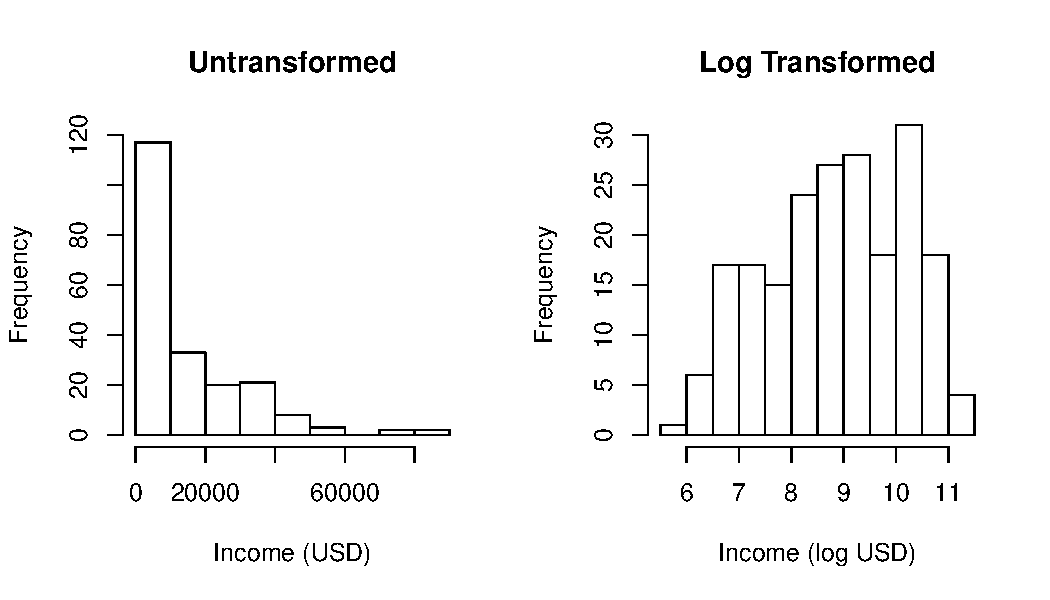
\includegraphics[width=\maxwidth]{figure/unnamed-chunk-28-1} 

\end{knitrout}

Transformations can also be applied to both variables when exploring a relationship. The following figure shows simplified versions of \textit{OI Biostat} Figures 1.23 and 1.27.

\begin{knitrout}
\definecolor{shadecolor}{rgb}{0.969, 0.969, 0.969}\color{fgcolor}\begin{kframe}
\begin{alltt}
\hlcom{## Figure 1.23 and Figure 1.27}
\hlkwd{par}\hlstd{(}\hlkwc{mfrow} \hlstd{=} \hlkwd{c}\hlstd{(}\hlnum{1}\hlstd{,} \hlnum{2}\hlstd{))}
\hlkwd{plot}\hlstd{(life.expectancy.income}\hlopt{$}\hlstd{income, life.expectancy.income}\hlopt{$}\hlstd{life.expectancy,}
    \hlkwc{ylab} \hlstd{=} \hlstr{"Life Expectancy (years)"}\hlstd{,} \hlkwc{xlab} \hlstd{=} \hlstr{"Per Capita Income (USD)"}\hlstd{,}
    \hlkwc{main} \hlstd{=} \hlstr{"Untransformed"}\hlstd{)}
\hlkwd{plot}\hlstd{(}\hlkwd{log}\hlstd{(life.expectancy.income}\hlopt{$}\hlstd{income),} \hlkwd{log}\hlstd{(life.expectancy.income}\hlopt{$}\hlstd{life.expectancy),}
    \hlkwc{ylab} \hlstd{=} \hlstr{"Life Expectancy (log years)"}\hlstd{,} \hlkwc{xlab} \hlstd{=} \hlstr{"Per Capita Income (log USD)"}\hlstd{,}
    \hlkwc{main} \hlstd{=} \hlstr{"Transformed"}\hlstd{)}
\end{alltt}
\end{kframe}
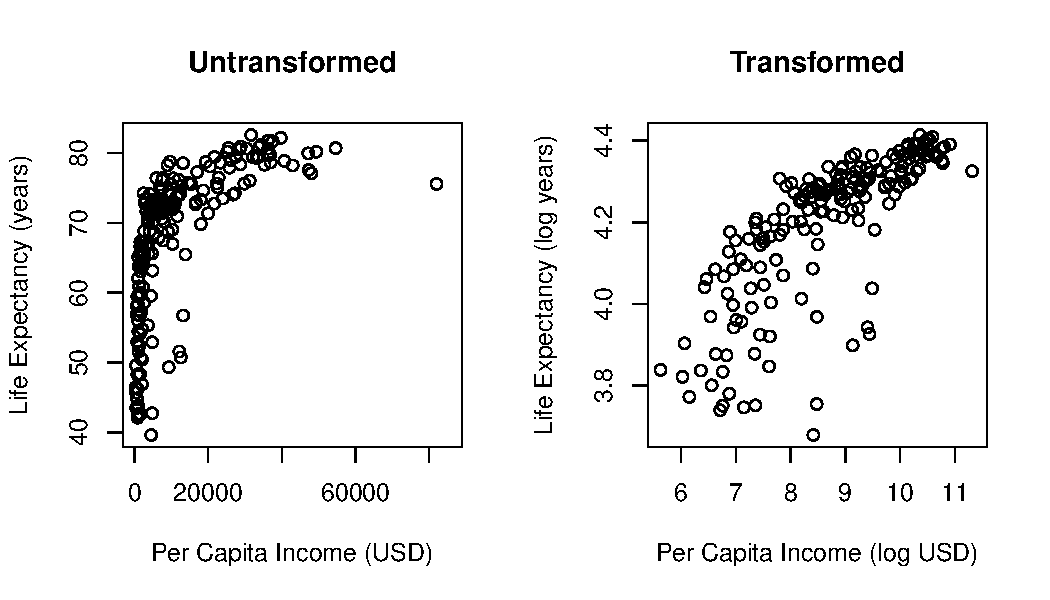
\includegraphics[width=\maxwidth]{figure/unnamed-chunk-29-1} 

\end{knitrout}

\section{Categorical Data}
\subsection{Contingency Tables}

A \textbf{frequency table} shows the counts for each category within a variable. The following \texttt{table()} command produces a frequency table for the \texttt{actn3.r577x} variable.

\begin{knitrout}
\definecolor{shadecolor}{rgb}{0.969, 0.969, 0.969}\color{fgcolor}\begin{kframe}
\begin{alltt}
\hlcom{## Table 1.28}
\hlkwd{addmargins}\hlstd{(}\hlkwd{table}\hlstd{(famuss}\hlopt{$}\hlstd{actn3.r577x))}
\end{alltt}
\begin{verbatim}
## 
##  CC  CT  TT Sum 
## 173 261 161 595
\end{verbatim}
\end{kframe}
\end{knitrout}

A \textbf{contingency table} summarizes data for two categorical variables, such as race and genotype in \textit{OI Biostat} Table 1.29. 

\begin{knitrout}
\definecolor{shadecolor}{rgb}{0.969, 0.969, 0.969}\color{fgcolor}\begin{kframe}
\begin{alltt}
\hlcom{## Table 1.29}
\hlkwd{addmargins}\hlstd{(}\hlkwd{table}\hlstd{(famuss}\hlopt{$}\hlstd{race, famuss}\hlopt{$}\hlstd{actn3.r577x))}
\end{alltt}
\begin{verbatim}
##             
##               CC  CT  TT Sum
##   African Am  16   6   5  27
##   Asian       21  18  16  55
##   Caucasian  125 216 126 467
##   Hispanic     4  10   9  23
##   Other        7  11   5  23
##   Sum        173 261 161 595
\end{verbatim}
\end{kframe}
\end{knitrout}

\textit{OI Biostat} Table 1.30 shows a contingency table with row proportions, computed as the counts divided by their row totals. The \texttt{prop.table()} command produces a table with row proportions, as specified by the \texttt{1} in the argument.

\begin{knitrout}
\definecolor{shadecolor}{rgb}{0.969, 0.969, 0.969}\color{fgcolor}\begin{kframe}
\begin{alltt}
\hlcom{## Table 1.30}
\hlstd{counts.table} \hlkwb{=} \hlkwd{table}\hlstd{(famuss}\hlopt{$}\hlstd{race, famuss}\hlopt{$}\hlstd{actn3.r577x)}
\hlstd{row.prop.table} \hlkwb{=} \hlkwd{prop.table}\hlstd{(counts.table,} \hlnum{1}\hlstd{)}
\hlstd{row.prop.table}
\end{alltt}
\begin{verbatim}
##             
##                     CC        CT        TT
##   African Am 0.5925926 0.2222222 0.1851852
##   Asian      0.3818182 0.3272727 0.2909091
##   Caucasian  0.2676660 0.4625268 0.2698073
##   Hispanic   0.1739130 0.4347826 0.3913043
##   Other      0.3043478 0.4782609 0.2173913
\end{verbatim}
\end{kframe}
\end{knitrout}

Alternatively, a contingency table can be created with column proportions by changing the \texttt{1} in \texttt{prop.table()} to a \texttt{2}. 

\begin{knitrout}
\definecolor{shadecolor}{rgb}{0.969, 0.969, 0.969}\color{fgcolor}\begin{kframe}
\begin{alltt}
\hlcom{## Table 1.31}
\hlstd{counts.table} \hlkwb{=} \hlkwd{table}\hlstd{(famuss}\hlopt{$}\hlstd{race, famuss}\hlopt{$}\hlstd{actn3.r577x)}
\hlstd{col.prop.table} \hlkwb{=} \hlkwd{prop.table}\hlstd{(counts.table,} \hlnum{2}\hlstd{)}
\hlstd{col.prop.table}
\end{alltt}
\begin{verbatim}
##             
##                      CC         CT         TT
##   African Am 0.09248555 0.02298851 0.03105590
##   Asian      0.12138728 0.06896552 0.09937888
##   Caucasian  0.72254335 0.82758621 0.78260870
##   Hispanic   0.02312139 0.03831418 0.05590062
##   Other      0.04046243 0.04214559 0.03105590
\end{verbatim}
\end{kframe}
\end{knitrout}

\subsection{Bar Plots}

A \textbf{bar plot} is a common way to display a single categorical variable, either from count data or from proportions. The \texttt{barplot()} command requires values to be input in a table format. In the below example, the \texttt{table()} command is nested within the \texttt{barplot()} command.

\begin{knitrout}
\definecolor{shadecolor}{rgb}{0.969, 0.969, 0.969}\color{fgcolor}\begin{kframe}
\begin{alltt}
\hlcom{## Figure 1.32}
\hlkwd{par}\hlstd{(}\hlkwc{mfrow} \hlstd{=} \hlkwd{c}\hlstd{(}\hlnum{1}\hlstd{,} \hlnum{2}\hlstd{))}
\hlkwd{barplot}\hlstd{(}\hlkwd{table}\hlstd{(famuss}\hlopt{$}\hlstd{actn3.r577x),} \hlkwc{main} \hlstd{=} \hlstr{"Count Barplot"}\hlstd{)}
\hlkwd{barplot}\hlstd{(}\hlkwd{table}\hlstd{(famuss}\hlopt{$}\hlstd{actn3.r577x)}\hlopt{/}\hlkwd{sum}\hlstd{(}\hlkwd{table}\hlstd{(famuss}\hlopt{$}\hlstd{actn3.r577x)),} \hlkwc{main} \hlstd{=} \hlstr{"Frequency Barplot"}\hlstd{)}  \hlcom{## frequency barplot}
\end{alltt}
\end{kframe}
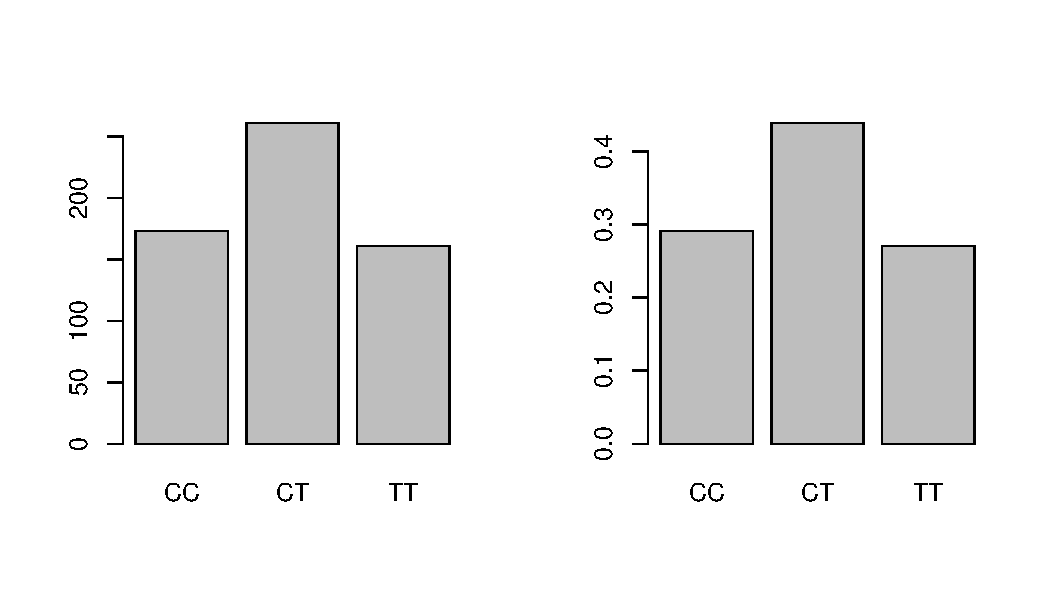
\includegraphics[width=\maxwidth]{figure/unnamed-chunk-34-1} 

\end{knitrout}

\newpage

\subsection{Segmented Bar Plot}

A \textbf{segmented bar plot} draws from a contingency table to display information about two categorical variables. The following code reproduces \textit{OI Biostat} Figure 1.33a, in which a bar plot was created using the \texttt{actn3.r577x} variable, with each group divided by the levels of race. The simplified version of the plot uses the default greyscale shading; it is also possible to specify a list of colors using \texttt{c()}. 

The argument \texttt{legend} can be used to specify whether the row names or the column names are used for the legend. 

\begin{knitrout}
\definecolor{shadecolor}{rgb}{0.969, 0.969, 0.969}\color{fgcolor}\begin{kframe}
\begin{alltt}
\hlcom{## Figure 1.31a First, create a table of the data that is}
\hlcom{## sorted}
\hlstd{genotype.race} \hlkwb{=} \hlkwd{matrix}\hlstd{(}\hlkwd{table}\hlstd{(famuss}\hlopt{$}\hlstd{actn3.r577x, famuss}\hlopt{$}\hlstd{race),}
    \hlkwc{ncol} \hlstd{=} \hlnum{3}\hlstd{,} \hlkwc{byrow} \hlstd{= T)}

\hlcom{# Second, change the column and row names on the table}
\hlkwd{colnames}\hlstd{(genotype.race)} \hlkwb{=} \hlkwd{c}\hlstd{(}\hlstr{"CC"}\hlstd{,} \hlstr{"CT"}\hlstd{,} \hlstr{"TT"}\hlstd{)}
\hlkwd{rownames}\hlstd{(genotype.race)} \hlkwb{=} \hlkwd{c}\hlstd{(}\hlstr{"African Am"}\hlstd{,} \hlstr{"Asian"}\hlstd{,} \hlstr{"Caucasian"}\hlstd{,}
    \hlstr{"Hispanic"}\hlstd{,} \hlstr{"Other"}\hlstd{)}

\hlcom{# Third, plot the barplot where colors are specified}
\hlkwd{barplot}\hlstd{(genotype.race,} \hlkwc{col} \hlstd{=} \hlkwd{c}\hlstd{(}\hlstr{"gray"}\hlstd{,} \hlstr{"firebrick1"}\hlstd{,} \hlstr{"dodgerblue"}\hlstd{,}
    \hlstr{"darkgreen"}\hlstd{,} \hlstr{"gold"}\hlstd{),} \hlkwc{ylim} \hlstd{=} \hlkwd{c}\hlstd{(}\hlnum{0}\hlstd{,} \hlnum{300}\hlstd{),} \hlkwc{width} \hlstd{=} \hlnum{2}\hlstd{,} \hlkwc{legend} \hlstd{=} \hlkwd{rownames}\hlstd{(counts.table))}
\end{alltt}
\end{kframe}

{\centering 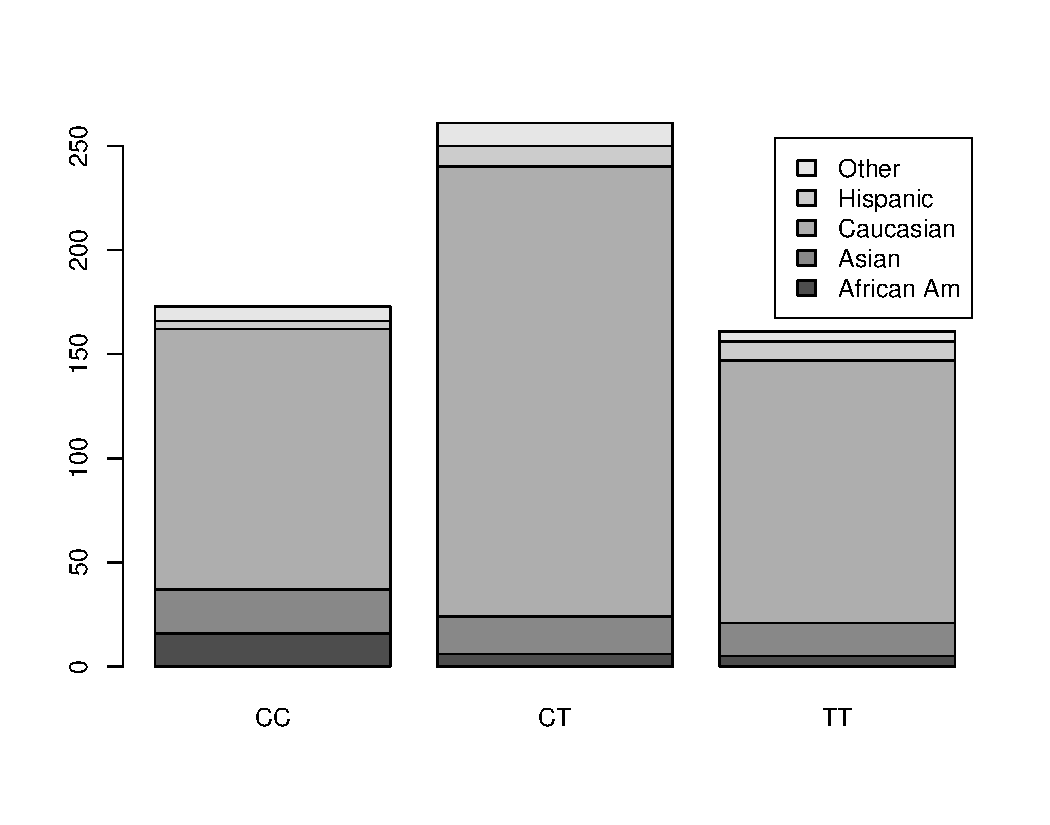
\includegraphics[width=\maxwidth]{figure/unnamed-chunk-35-1} 

}



\end{knitrout}

\newpage

A \textbf{standardized segmented bar plot} uses proportions to scale the data, and draws from a contingency table with proportions. Setting \texttt{ylim} from 0 to 1.7 allows for enough empty space on the plot so that the legend does not overlap the bars.

\begin{knitrout}
\definecolor{shadecolor}{rgb}{0.969, 0.969, 0.969}\color{fgcolor}\begin{kframe}
\begin{alltt}
\hlcom{## Figure 1.33b}
\hlstd{counts.table} \hlkwb{=} \hlstd{(}\hlkwd{table}\hlstd{(famuss}\hlopt{$}\hlstd{race, famuss}\hlopt{$}\hlstd{actn3.r577x))}
\hlstd{row.prop.table} \hlkwb{=} \hlkwd{prop.table}\hlstd{(counts.table,} \hlnum{2}\hlstd{)}

\hlkwd{barplot}\hlstd{(row.prop.table,} \hlkwc{col} \hlstd{=} \hlkwd{c}\hlstd{(}\hlstr{"gray"}\hlstd{,} \hlstr{"firebrick1"}\hlstd{,} \hlstr{"dodgerblue"}\hlstd{,}
    \hlstr{"darkgreen"}\hlstd{,} \hlstr{"gold"}\hlstd{),} \hlkwc{ylim} \hlstd{=} \hlkwd{c}\hlstd{(}\hlnum{0}\hlstd{,} \hlnum{1.7}\hlstd{),} \hlkwc{legend} \hlstd{=} \hlkwd{rownames}\hlstd{(counts.table))}
\end{alltt}
\end{kframe}

{\centering 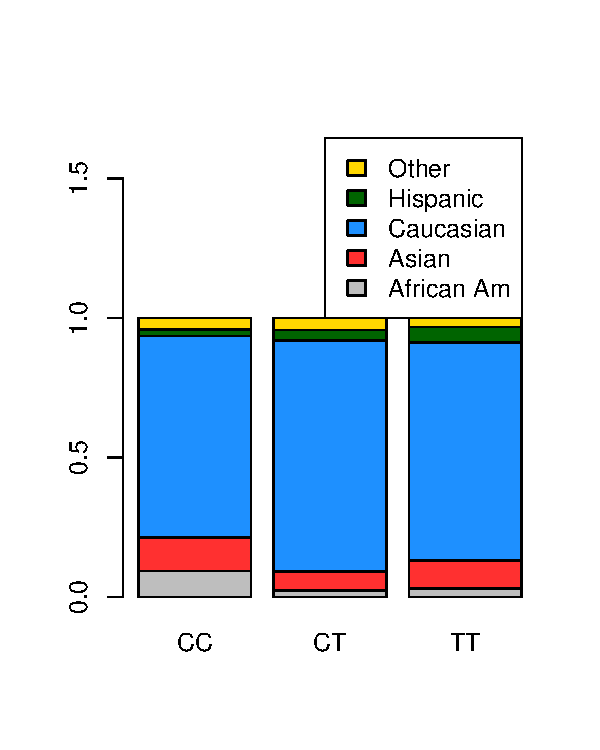
\includegraphics[width=\maxwidth]{figure/unnamed-chunk-36-1} 

}



\end{knitrout}

\begin{knitrout}
\definecolor{shadecolor}{rgb}{0.969, 0.969, 0.969}\color{fgcolor}\begin{kframe}
\begin{alltt}
\hlcom{## Figure 1.31b First, create table of proportions}
\hlstd{prop.genotype.race} \hlkwb{<-} \hlkwd{prop.table}\hlstd{(genotype.race,} \hlnum{2}\hlstd{)}

\hlcom{# Second, change the column and row names on the table}
\hlkwd{colnames}\hlstd{(prop.genotype.race)} \hlkwb{=} \hlkwd{c}\hlstd{(}\hlstr{"CC"}\hlstd{,} \hlstr{"CT"}\hlstd{,} \hlstr{"TT"}\hlstd{)}
\hlkwd{rownames}\hlstd{(prop.genotype.race)} \hlkwb{=} \hlkwd{c}\hlstd{(}\hlstr{"African Am"}\hlstd{,} \hlstr{"Asian"}\hlstd{,} \hlstr{"Caucasian"}\hlstd{,}
    \hlstr{"Hispanic"}\hlstd{,} \hlstr{"Other"}\hlstd{)}

\hlcom{# Third, plot the output}
\hlkwd{barplot}\hlstd{(prop.genotype.race,} \hlkwc{col} \hlstd{=} \hlkwd{c}\hlstd{(}\hlstr{"gray"}\hlstd{,} \hlstr{"firebrick1"}\hlstd{,} \hlstr{"dodgerblue"}\hlstd{,}
    \hlstr{"darkgreen"}\hlstd{,} \hlstr{"gold"}\hlstd{),} \hlkwc{ylim} \hlstd{=} \hlkwd{c}\hlstd{(}\hlnum{0}\hlstd{,} \hlnum{1.7}\hlstd{),} \hlkwc{width} \hlstd{=} \hlnum{2}\hlstd{,} \hlkwc{legend} \hlstd{=} \hlkwd{rownames}\hlstd{(counts.table))}
\end{alltt}
\end{kframe}

{\centering 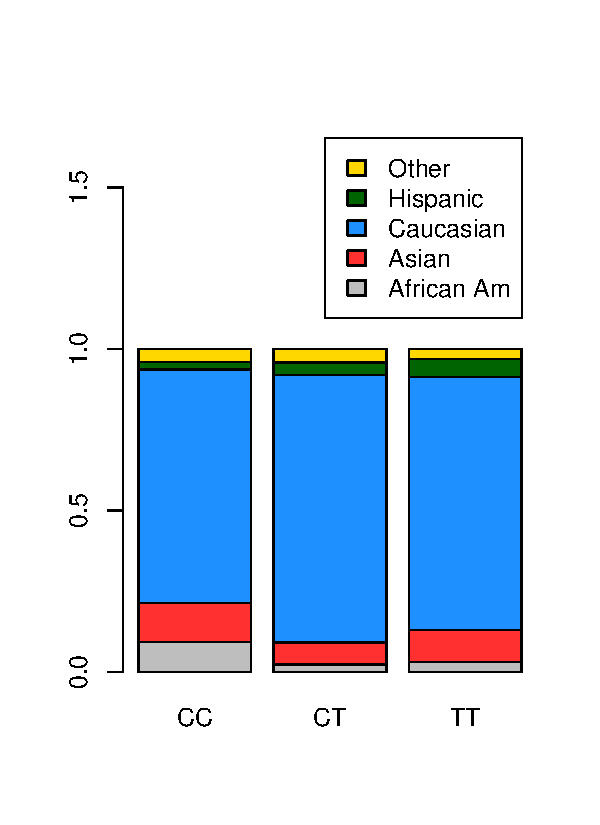
\includegraphics[width=\maxwidth]{figure/unnamed-chunk-37-1} 

}



\end{knitrout}

In \textit{OI Biostat} Figure 1.34, the data from the contingency table are organized differently, with each bar representing a level of \texttt{race}. To make this change, reverse the order of the variables in \texttt{table()}

\begin{knitrout}
\definecolor{shadecolor}{rgb}{0.969, 0.969, 0.969}\color{fgcolor}\begin{kframe}
\begin{alltt}
\hlcom{## Figure 1.34 Plotting two graphs next to each other}
\hlkwd{par}\hlstd{(}\hlkwc{mfrow} \hlstd{= (}\hlkwd{c}\hlstd{(}\hlnum{1}\hlstd{,} \hlnum{2}\hlstd{)))}

\hlcom{# Setting up the table and changing column/row names}
\hlstd{race.genotype} \hlkwb{=} \hlkwd{matrix}\hlstd{(}\hlkwd{table}\hlstd{(famuss}\hlopt{$}\hlstd{race, famuss}\hlopt{$}\hlstd{actn3.r577x),}
    \hlkwc{ncol} \hlstd{=} \hlnum{5}\hlstd{,} \hlkwc{byrow} \hlstd{= T)}
\hlkwd{colnames}\hlstd{(race.genotype)} \hlkwb{=} \hlkwd{c}\hlstd{(}\hlstr{"African Am"}\hlstd{,} \hlstr{"Asian"}\hlstd{,} \hlstr{"Caucasian"}\hlstd{,}
    \hlstr{"Hispanic"}\hlstd{,} \hlstr{"Other"}\hlstd{)}
\hlkwd{rownames}\hlstd{(race.genotype)} \hlkwb{=} \hlkwd{c}\hlstd{(}\hlstr{"CC"}\hlstd{,} \hlstr{"CT"}\hlstd{,} \hlstr{"TT"}\hlstd{)}

\hlcom{# Creating segmented bar plot (Figure 1.34a)}
\hlkwd{barplot}\hlstd{(race.genotype,} \hlkwc{col} \hlstd{=} \hlkwd{c}\hlstd{(}\hlstr{"dodgerblue"}\hlstd{,} \hlstr{"darkgreen"}\hlstd{,} \hlstr{"gold"}\hlstd{),}
    \hlkwc{ylim} \hlstd{=} \hlkwd{c}\hlstd{(}\hlnum{0}\hlstd{,} \hlnum{500}\hlstd{),} \hlkwc{width} \hlstd{=} \hlnum{2}\hlstd{,} \hlkwc{legend} \hlstd{=} \hlkwd{rownames}\hlstd{(race.genotype))}

\hlcom{# Creating standardized segmented bar plot (Figure 1.34b)}
\hlstd{prop.race.genotype} \hlkwb{<-} \hlkwd{prop.table}\hlstd{(race.genotype,} \hlnum{2}\hlstd{)}
\hlkwd{barplot}\hlstd{(prop.race.genotype,} \hlkwc{col} \hlstd{=} \hlkwd{c}\hlstd{(}\hlstr{"dodgerblue"}\hlstd{,} \hlstr{"darkgreen"}\hlstd{,}
    \hlstr{"gold"}\hlstd{),} \hlkwc{ylim} \hlstd{=} \hlkwd{c}\hlstd{(}\hlnum{0}\hlstd{,} \hlnum{1.7}\hlstd{),} \hlkwc{width} \hlstd{=} \hlnum{2}\hlstd{,} \hlkwc{legend} \hlstd{=} \hlkwd{rownames}\hlstd{(race.genotype))}
\end{alltt}
\end{kframe}

{\centering 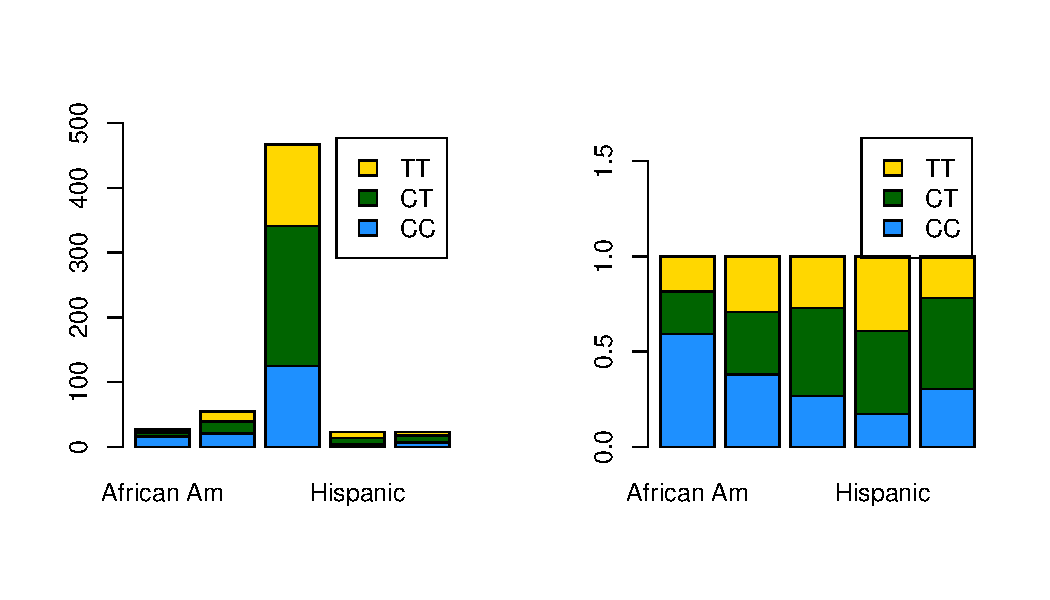
\includegraphics[width=\maxwidth]{figure/unnamed-chunk-38-1} 

}



\end{knitrout}

\subsection{Comparing numerical data across groups}
\subsubsection{Side-by-side boxplots}

The \textbf{side-by-side} boxplot is a useful tool for comparing the distribution of numerical data across categories. \textit{OI Biostat} Figure 1.35a shows a side-by-side boxplot for percent change in non-dominant arm strength grouped by genotype. The response variable $y$ comes before the tilde and the explanatory variable $x$; in this case, the response variable is percent change in strength.

\begin{knitrout}
\definecolor{shadecolor}{rgb}{0.969, 0.969, 0.969}\color{fgcolor}\begin{kframe}
\begin{alltt}
\hlcom{## Figure 1.35(a)}
\hlkwd{boxplot}\hlstd{(famuss}\hlopt{$}\hlstd{ndrm.ch} \hlopt{~} \hlstd{famuss}\hlopt{$}\hlstd{actn3.r577x,}
    \hlkwc{ylab} \hlstd{=} \hlstr{"% Change in Non-Dominant Arm Strength"}\hlstd{,}
    \hlkwc{xlab} \hlstd{=} \hlstr{"Genotype"}\hlstd{)}
\end{alltt}
\end{kframe}

{\centering 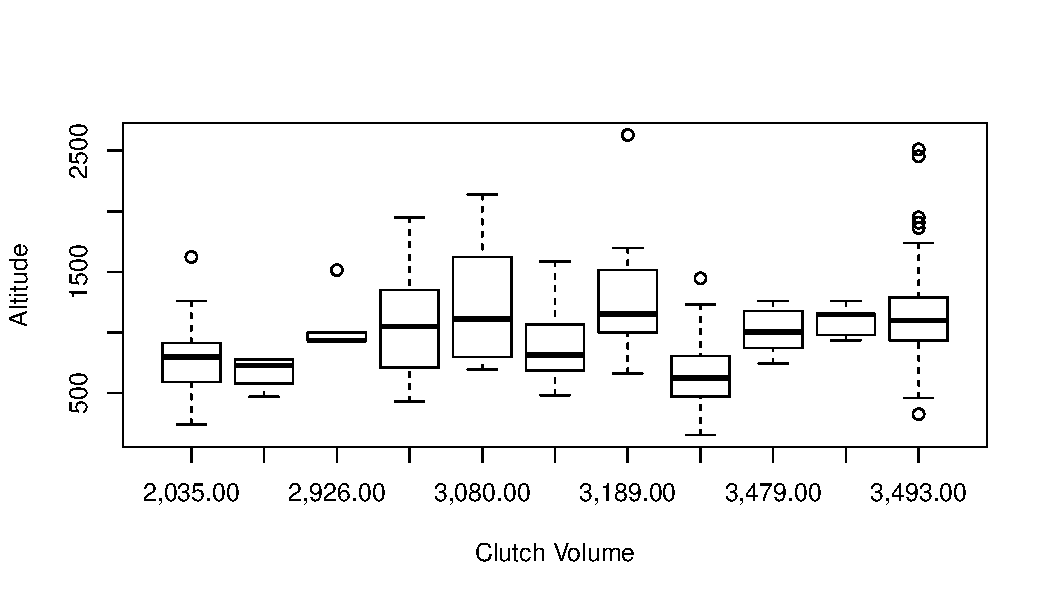
\includegraphics[width=\maxwidth]{figure/unnamed-chunk-39-1} 

}



\end{knitrout}

\textit{OI Biostat} Figure 1.36 shows a larger side-by-side boxplot which compares the distribution of frog clutch sizes for different altitudes.

\begin{knitrout}
\definecolor{shadecolor}{rgb}{0.969, 0.969, 0.969}\color{fgcolor}\begin{kframe}
\begin{alltt}
\hlcom{## Figure 1.36}
\hlkwd{boxplot}\hlstd{(frog.altitude.data}\hlopt{$}\hlstd{clutch.volume} \hlopt{~} \hlstd{frog.altitude.data}\hlopt{$}\hlstd{altitude,}
    \hlkwc{xlab} \hlstd{=} \hlstr{"Clutch Volume"}\hlstd{,} \hlkwc{ylab} \hlstd{=} \hlstr{"Altitude"}\hlstd{)}
\end{alltt}
\end{kframe}

{\centering 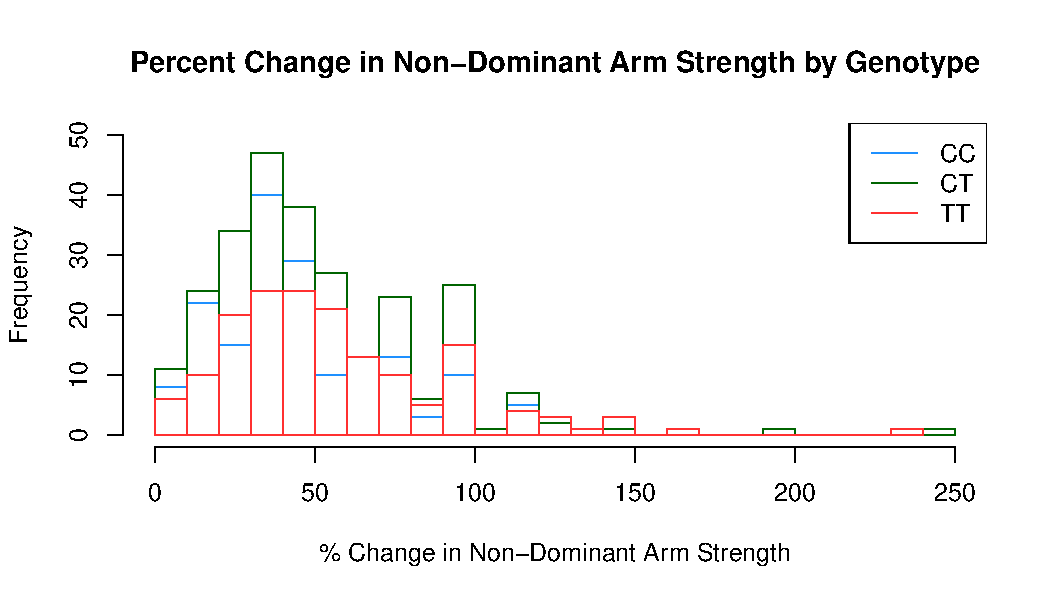
\includegraphics[width=\maxwidth]{figure/unnamed-chunk-40-1} 

}



\end{knitrout}

\subsubsection{Hollow Histograms}

A \textbf{hollow histogram} plots the outlines of histograms for each group onto the same axes. To plot a hollow histogram, specify any axis limits and labels in the command for the first histogram; the subsequent histograms require the argument \texttt{add = T} in order for them to be overlaid on top of the first plot.

\begin{knitrout}
\definecolor{shadecolor}{rgb}{0.969, 0.969, 0.969}\color{fgcolor}\begin{kframe}
\begin{alltt}
\hlcom{## Figure 1.35(b)}
\hlkwd{hist}\hlstd{(famuss}\hlopt{$}\hlstd{ndrm.ch[famuss}\hlopt{$}\hlstd{actn3.r577x} \hlopt{==} \hlstr{"CC"}\hlstd{],} \hlkwc{breaks} \hlstd{=} \hlnum{20}\hlstd{,} \hlkwc{border} \hlstd{=} \hlstr{"dodgerblue"}\hlstd{,}
     \hlkwc{xlab} \hlstd{=} \hlstr{"% Change in Non-Dominant Arm Strength"}\hlstd{,} \hlkwc{ylim} \hlstd{=} \hlkwd{c}\hlstd{(}\hlnum{0}\hlstd{,}\hlnum{50}\hlstd{),} \hlkwc{xlim} \hlstd{=} \hlkwd{c}\hlstd{(}\hlnum{0}\hlstd{,}\hlnum{250}\hlstd{),}
     \hlkwc{main} \hlstd{=} \hlstr{"Percent Change in Non-Dominant Arm Strength by Genotype"}\hlstd{)}
\hlkwd{hist}\hlstd{(famuss}\hlopt{$}\hlstd{ndrm.ch[famuss}\hlopt{$}\hlstd{actn3.r577x} \hlopt{==} \hlstr{"CT"}\hlstd{],} \hlkwc{breaks} \hlstd{=} \hlnum{20}\hlstd{,} \hlkwc{border} \hlstd{=} \hlstr{"darkgreen"}\hlstd{,}
     \hlkwc{add} \hlstd{= T)}
\hlkwd{hist}\hlstd{(famuss}\hlopt{$}\hlstd{ndrm.ch[famuss}\hlopt{$}\hlstd{actn3.r577x} \hlopt{==} \hlstr{"TT"}\hlstd{],} \hlkwc{breaks} \hlstd{=} \hlnum{20}\hlstd{,} \hlkwc{border} \hlstd{=} \hlstr{"firebrick1"}\hlstd{,}
     \hlkwc{add} \hlstd{= T)}

\hlkwd{legend}\hlstd{(}\hlstr{'topright'}\hlstd{,}
       \hlkwc{col} \hlstd{=} \hlkwd{c}\hlstd{(}\hlstr{"dodgerblue"}\hlstd{,} \hlstr{"darkgreen"}\hlstd{,} \hlstr{"firebrick1"}\hlstd{),}
       \hlkwc{lwd} \hlstd{=} \hlkwd{c}\hlstd{(}\hlnum{1}\hlstd{,} \hlnum{1}\hlstd{,} \hlnum{1}\hlstd{),}     \hlcom{## line width}
       \hlkwc{legend} \hlstd{=} \hlkwd{c}\hlstd{(}\hlstr{'CC'}\hlstd{,} \hlstr{'CT'}\hlstd{,} \hlstr{'TT'}\hlstd{))}    \hlcom{##legend labels}
\end{alltt}
\end{kframe}

{\centering 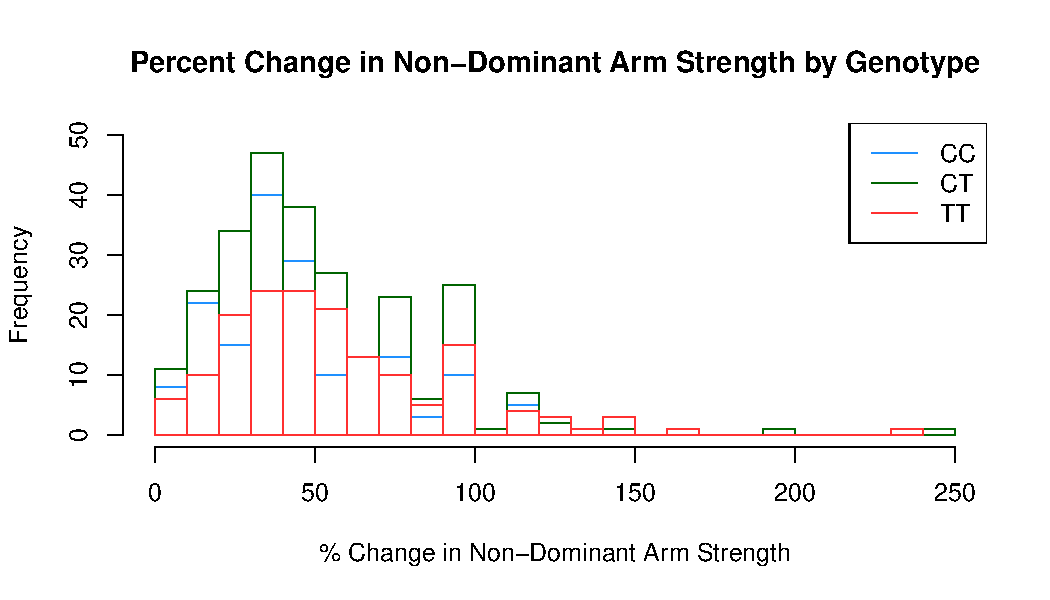
\includegraphics[width=\maxwidth]{figure/unnamed-chunk-41-1} 

}



\end{knitrout}

\section{Genomic Data}

% JV: Golub data (golub_exprs_pheno) needs to be added to the package

% JV: Add material from 102 section 2 to this section, as an exercise? Doesn't seem useful to just reproduce the figures in OI Biostat 1.6 here.

\begin{knitrout}
\definecolor{shadecolor}{rgb}{0.969, 0.969, 0.969}\color{fgcolor}\begin{kframe}
\begin{alltt}
\hlkwd{boxplot}\hlstd{(Golub[,} \hlnum{7}\hlopt{:}\hlnum{9}\hlstd{])}
\end{alltt}
\end{kframe}

{\centering 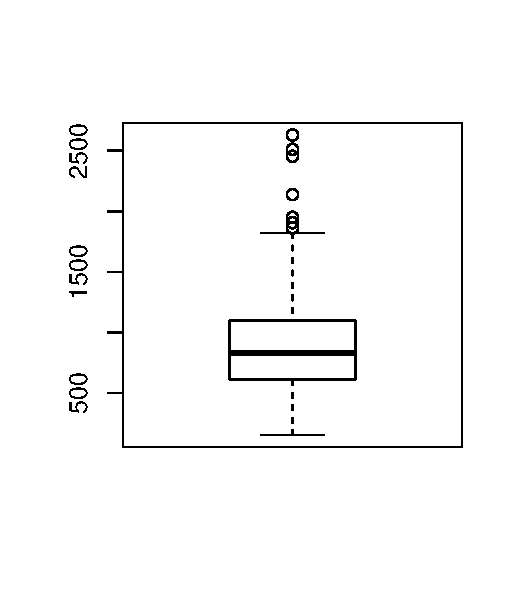
\includegraphics[width=\maxwidth]{figure/unnamed-chunk-42-1} 

}



\end{knitrout}


\newpage 
\chapter{Using R for Probabilities}
\minitoc

\vspace{0.5cm} 

This chapter focuses on the material covered in \textit{OI Biostat} Chapter 2, which focuses on the idea of probability and how to solve for various types of probabilities. This chapter will work through several examples, illustrating how \textsf{R} can be used to solve propability problems.  Once again, it will be shown that there are several different computational methods that can be used to answer the same question.  

\section{Simple Probability}

\subsection{Using R as a Calculator}
For the most basic probability problems, \textsf{R} can be used similarly to a calculator.  Variable values can be stored and then used for calculations.  An example of this is \textit{OI Biostat} Example 2.24, which is walked through below.   

\begin{quotation}
\textbf{\textit{OI Biostat} Example 2.24.}  Mandatory drug testing in the workplace is common practice for certain professions, such as air traffic controllers and transportation workers.  A false positive in a drug screening test occurs when the test incorrectly indicates that a screened person is an illegal drug user. Suppose a mandatory drug test has a false positive rate of 1.2\% (i.e., has probability  0.012 of indicating that an employee is using illegal drugs when that is not the case).  Given 150 employees who are in reality drug free, what is the probability that at least one will (falsely) test positive? Assume that the outcome of one drug test has no effect on the others.
\end{quotation}

\begin{knitrout}
\definecolor{shadecolor}{rgb}{0.969, 0.969, 0.969}\color{fgcolor}\begin{kframe}
\begin{alltt}
\hlcom{## Example 2.24}
\hlstd{false.positive} \hlkwb{=} \hlnum{0.012}
\hlstd{true.negative} \hlkwb{=} \hlnum{1}\hlopt{-}\hlstd{false.positive}
\hlstd{one.positive} \hlkwb{=} \hlnum{1}\hlopt{-}\hlstd{true.negative}\hlopt{^}\hlnum{150}
\hlstd{one.positive}
\end{alltt}
\begin{verbatim}
## [1] 0.836491
\end{verbatim}
\end{kframe}
\end{knitrout}


\subsection{Through Simulation}
A powerful method for calculating probabilities in \textsf{R} is called \textbf{simulation} and consists of simulating a large population with some consistent known parameters so that population statistics can be measured.   

The steps for a simulation process are as follows, 
\begin{enumerate}
  \item Define the parameters of the simulation: population size.
  
  \item In order for the results of the simulation to be reproducible, it is necessary to use \texttt{set.seed()} to associate the particular set of results with a "seed". Any integer can be used as the seed. Different seeds will produce a different set of results. 
  
  \item Using the \texttt{vector()} command, create one empty list that will be used to store the results of the simulation.  
  
  \item Simulate rolling each of the dice using the  \texttt{sample()} command, which takes a sample of a specified size from a list \texttt{x}. In this context, the goal is to sample the integers between \texttt{1} and \texttt{6} 100,000 times, where the result represents the face of the die that shows up.  This is done in combination with a \texttt{for} loop.  The loop allows for this process to be repeated for each of the 100,000 individuals being simulated.  The first line sets up the loop, with a variable \texttt{ii} that starts at \texttt{1} and finishes at \texttt{population.size}, which was specified earlier as 100,000. This allows for each dice roll to be performed one at a time.
  
  \item Look at your final results of the simulated population distribution, and if desired, calculate population statistics. 

\end{enumerate}

\subsubsection{Dice Rolling Example}
For example, simulation can be used to obtain the probability distribution of the sum of two dice seen in \textit{OI Biostat} Figure 2.7. Note that these probabilities can be calculatd directly as well, as shown in \textit{OI Biostat}.  

\begin{knitrout}
\definecolor{shadecolor}{rgb}{0.969, 0.969, 0.969}\color{fgcolor}\begin{kframe}
\begin{alltt}
\hlcom{## 1. Set parameters}
\hlstd{population.size} \hlkwb{=} \hlnum{1e+05}

\hlcom{## 2. Set Seed}
\hlkwd{set.seed}\hlstd{(}\hlnum{2016}\hlstd{)}

\hlcom{## 3. Create empty list}
\hlstd{dice.sums} \hlkwb{=} \hlkwd{vector}\hlstd{(}\hlstr{"numeric"}\hlstd{, population.size)}

\hlcom{## 4. Simulate 'rolling the dice'}
\hlkwa{for} \hlstd{(ii} \hlkwa{in} \hlnum{1}\hlopt{:}\hlstd{population.size) \{}
    \hlstd{dice.1} \hlkwb{=} \hlkwd{sample}\hlstd{(}\hlnum{1}\hlopt{:}\hlnum{6}\hlstd{,} \hlkwc{size} \hlstd{=} \hlnum{1}\hlstd{)}
    \hlstd{dice.2} \hlkwb{=} \hlkwd{sample}\hlstd{(}\hlnum{1}\hlopt{:}\hlnum{6}\hlstd{,} \hlkwc{size} \hlstd{=} \hlnum{1}\hlstd{)}
    \hlstd{dice.sums[ii]} \hlkwb{=} \hlstd{dice.1} \hlopt{+} \hlstd{dice.2}
\hlstd{\}}

\hlcom{## 5. Plot results}
\hlkwd{hist}\hlstd{(dice.sums,} \hlkwc{freq} \hlstd{=} \hlnum{FALSE}\hlstd{,} \hlkwc{ylab} \hlstd{=} \hlstr{"Probability"}\hlstd{,} \hlkwc{xlab} \hlstd{=} \hlstr{"Dice Sum"}\hlstd{,} \hlkwc{main} \hlstd{=} \hlstr{""}\hlstd{)}
\end{alltt}
\end{kframe}

{\centering 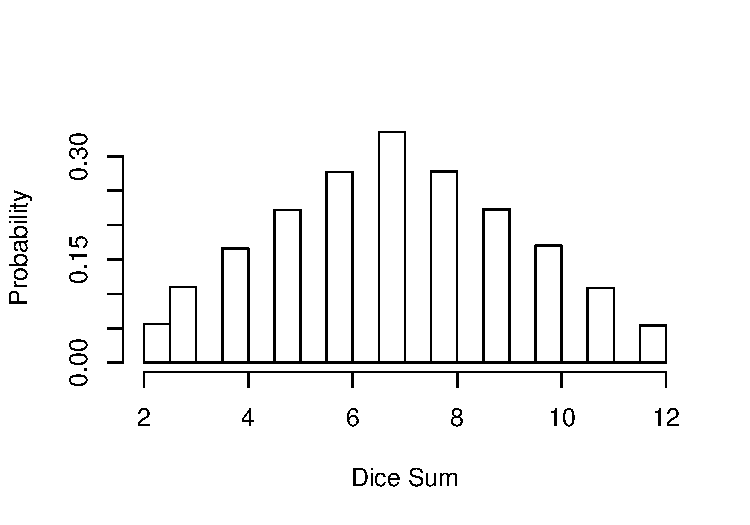
\includegraphics[width=\maxwidth]{figure/unnamed-chunk-44-1} 

}



\end{knitrout}

\subsubsection{Drug Testing Example}
Another example of a probability that can be calculated using simulation is \textit{OI Biostat} Example 2.24, which was calculated directly above.  In the \texttt{sample} command here, a result of 0 indicates a negative test result while a result of 1 indicates a positive test, and the inclusion of \texttt{replace = TRUE} ensures that each individual's test is independent of the others.  

\begin{knitrout}
\definecolor{shadecolor}{rgb}{0.969, 0.969, 0.969}\color{fgcolor}\begin{kframe}
\begin{alltt}
\hlcom{## 1. Set parameters }
\hlstd{simulation.size} \hlkwb{=} \hlnum{100000}
\hlstd{n} \hlkwb{=} \hlnum{150}
\hlstd{false.positive} \hlkwb{=} \hlnum{0.012}

\hlcom{## 2. Set Seed }
\hlkwd{set.seed}\hlstd{(}\hlnum{2016}\hlstd{)}

\hlcom{## 3. Create empty list }
\hlstd{test.results} \hlkwb{=} \hlkwd{vector}\hlstd{(}\hlstr{"numeric"}\hlstd{, population.size)}

\hlcom{## 4. Simulate "rolling the dice" }
\hlkwa{for}\hlstd{(ii} \hlkwa{in} \hlnum{1}\hlopt{:}\hlstd{population.size)\{}
  \hlcom{## Simulate the 150 employee's test results}
  \hlstd{employees} \hlkwb{=} \hlkwd{sample}\hlstd{(}\hlkwd{c}\hlstd{(}\hlnum{0}\hlstd{,}\hlnum{1}\hlstd{),} \hlkwc{size} \hlstd{= n,} \hlkwc{prob} \hlstd{=} \hlkwd{c}\hlstd{(}\hlnum{1}\hlopt{-}\hlstd{false.positive, false.positive),} \hlkwc{replace} \hlstd{=} \hlnum{TRUE}\hlstd{)}
  \hlcom{## Count how many employees tested positive }
  \hlstd{test.results[ii]} \hlkwb{=} \hlkwd{sum}\hlstd{(employees)}
\hlstd{\}}

\hlcom{## 5. Obtain results }
\hlkwd{mean}\hlstd{(test.results}\hlopt{>=}\hlnum{1}\hlstd{)}
\end{alltt}
\begin{verbatim}
## [1] 0.83584
\end{verbatim}
\end{kframe}
\end{knitrout}


\section{Conditional Probability}
What are the chances that a woman with a positive mamogram has breast cancer? This question can be rephrased as the conditional probability that a woman has breast cancer, given that her mammogram is abnormal, otherwise known as the \textbf{positive predictive value} of a mammogram. Two methods discussed in this chapter, using Bayes' Theorem and creating a contingency table, are also explained in \textit{OI Biostat}. This chapter will also cover an additional approach: modeling the problem scenario by running a simulation.

\begin{quotation}

\textbf{\textit{OI Biostat} Example 2.37.} In Canada, about 0.35\% of women over 40 will develop breast cancer in any given year. A common screening test for cancer is the mammogram, but it is not perfect. In about 11\% of patients with breast cancer, the test gives a \textbf{false negative}: it indicates a woman does not have breast cancer when she does have breast cancer. Similarly, the test gives a \textbf{false positive} in 7\% of patients who do not have breast cancer: it indicates these patients have breast cancer when they actually do not. If a randomly selected woman over 40 is tested for breast cancer using a mammogram and the test is positive -- that is, the test suggests the woman has cancer -- what is the probability she has breast cancer?

\end{quotation}

\subsection{Bayes' Theorem}

Bayes' Theorem states that the conditional probability $P(A_1 | B)$ can be identified as the following fraction:\vspace{-1.5mm}
\begin{align*}
\frac{P(A_1 \text{and } B)}{P(B)}= \frac{P(B | A_1) P(A_1)}
	{P(B | A_1) P(A_1) + P(B | A_2) P(A_2) + \cdots + P(B | A_k) P(A_k)}
\end{align*}
where $A_2$, $A_3$, ..., and $A_k$ represent all other possible outcomes of the first variable.

The expression can also be written in terms of diagnostic testing language, where $D = \text{\{has disease\}}$, $D^c = \text{\{does not have disease\}}$, $T^{+} = \text{\{positive test result\}}$, and $T^{-} = \text{\{negative test result\}}$.

\begin{align*}
P(D|T^{+}) &= \dfrac{P(D \text{ and } T^{+})}{P(D)} \\
&= \dfrac{P(T^{+}|D) \times P(D)}{[P(T^{+}|D) \times P(D)] + [P(T^{+}|D^c) \times P(D^c)]} \\
\text{PPV} &= \dfrac{\text{sensitivity } \times \text{ prevalence}}{[\text{sensitivity } \times \text{ prevalence}] + [\text{(1 - specificity) } \times \text{ (1 - prevalence)}]}
\end{align*}

\textsf{R} can be used to store values for prevalence, sensitivity, and specificity so that calculations are less tedious. Recall that the \textbf{sensitivity} is the probability of a positive test result when disease is present, which is the complement of a false negative. The \textbf{specificity} is the probability of a negative test result when disease is absent, which is the complement of a false positive.  With this in mind, solving for the \textbf{positive predictive value (PPV)} is quite easy in \textsf{R} for the breast cancer example as follows.  

\begin{knitrout}
\definecolor{shadecolor}{rgb}{0.969, 0.969, 0.969}\color{fgcolor}\begin{kframe}
\begin{alltt}
\hlstd{prevalence} \hlkwb{=} \hlnum{0.0035}
\hlstd{sensitivity} \hlkwb{=} \hlnum{1} \hlopt{-} \hlnum{0.11}
\hlstd{specificity} \hlkwb{=} \hlnum{1} \hlopt{-} \hlnum{0.07}

\hlstd{ppv.num} \hlkwb{=} \hlstd{(sensitivity}\hlopt{*}\hlstd{prevalence)}  \hlcom{## numerator}
\hlstd{ppv.den} \hlkwb{=} \hlstd{ppv.num} \hlopt{+} \hlstd{((}\hlnum{1}\hlopt{-}\hlstd{specificity)}\hlopt{*}\hlstd{(}\hlnum{1}\hlopt{-}\hlstd{prevalence))}  \hlcom{## denominator}
\hlstd{ppv} \hlkwb{=} \hlstd{ppv.num} \hlopt{/} \hlstd{ppv.den}

\hlstd{ppv}
\end{alltt}
\begin{verbatim}
## [1] 0.04274736
\end{verbatim}
\end{kframe}
\end{knitrout}


\subsection{Contingency Table}

The PPV can also be calculated by constructing a two-way contingency table for a hypothetical population and calculating conditional probabilities by conditioning on rows or columns. While this method results in an estimate of PPV, using a large enough population size such as 100,000 produces an empirical estimate that is very close to the exact value found through using Bayes' Theorem. 

\begin{center}
\begin{tabular}{|l|c|c|r|}
\hline 
& D+ & D- & Total\\ 
\hline
T+ & & & \\ 
\hline
T- & & & \\ 
\hline 
Total & & & 100,000 \\ 
\hline 
\end{tabular} 
\end{center} 

First, calculate the expected number of disease cases and non-disease cases in the population:
\begin{knitrout}
\definecolor{shadecolor}{rgb}{0.969, 0.969, 0.969}\color{fgcolor}\begin{kframe}
\begin{alltt}
\hlstd{population.size} \hlkwb{=} \hlnum{100000}
\hlstd{expected.cases} \hlkwb{=} \hlstd{prevalence} \hlopt{*} \hlstd{population.size}
\hlstd{expected.cases}
\end{alltt}
\begin{verbatim}
## [1] 350
\end{verbatim}
\begin{alltt}
\hlstd{expected.noncases} \hlkwb{=} \hlstd{(}\hlnum{1} \hlopt{-} \hlstd{prevalence)} \hlopt{*} \hlstd{population.size}
\hlstd{expected.noncases}
\end{alltt}
\begin{verbatim}
## [1] 99650
\end{verbatim}
\end{kframe}
\end{knitrout}

\begin{center}
\begin{tabular}{|l|c|c|r|}
\hline 
& D+ & D- & Total\\ 
\hline
T+ & & & \\ 
\hline
T- & & & \\ 
\hline 
Total & 350 & 99,650 & 100,000 \\ 
\hline 
\end{tabular} 
\end{center}

Next, calculate the expected number of cases of true positives and the expected number of cases of false positives:  
\begin{knitrout}
\definecolor{shadecolor}{rgb}{0.969, 0.969, 0.969}\color{fgcolor}\begin{kframe}
\begin{alltt}
\hlstd{expected.true.positives} \hlkwb{=} \hlstd{expected.cases} \hlopt{*} \hlstd{sensitivity}
\hlstd{expected.true.positives}
\end{alltt}
\begin{verbatim}
## [1] 311.5
\end{verbatim}
\begin{alltt}
\hlstd{expected.false.positives} \hlkwb{=} \hlstd{expected.noncases} \hlopt{*} \hlstd{(}\hlnum{1} \hlopt{-} \hlstd{specificity)}
\hlstd{expected.false.positives}
\end{alltt}
\begin{verbatim}
## [1] 6975.5
\end{verbatim}
\begin{alltt}
\hlstd{total.expected.positives} \hlkwb{=} \hlstd{expected.true.positives} \hlopt{+} \hlstd{expected.false.positives}
\hlstd{total.expected.positives}
\end{alltt}
\begin{verbatim}
## [1] 7287
\end{verbatim}
\end{kframe}
\end{knitrout}

 
\begin{center}
\begin{tabular}{|l|c|c|r|}
\hline 
& D+ & D- & Total\\ 
\hline
T+ & 311.5 & 6,975.5 & 7,287\\ 
\hline
T- & & & \\ 
\hline 
Total & 350 & 99,650 & 100,000 \\ 
\hline 
\end{tabular} 
\end{center}

Finally, calculate the positive predictive value: 
\begin{knitrout}
\definecolor{shadecolor}{rgb}{0.969, 0.969, 0.969}\color{fgcolor}\begin{kframe}
\begin{alltt}
\hlstd{ppv} \hlkwb{=} \hlstd{expected.true.positives}\hlopt{/}\hlstd{total.expected.positives}
\hlstd{ppv}
\end{alltt}
\begin{verbatim}
## [1] 0.04274736
\end{verbatim}
\end{kframe}
\end{knitrout}


\subsection{Simulation}

% JV: will definitely be good to have some simple simulation exercises for this chapter, like the drug testing example from 102

The final method for solving this conditional probability problem in \textsf{R} is through \textbf{simulation} and involves the process of simulating 100,000 individuals who each have the same probability of having the disease.  Afterwards, using the known specificity and sensitivity of the diagnostic test, individuals can be assigned a test result of either positve or negative as if a test had been performed.  This results in a simulated dataset of 100,000 individuals that each have a disease status and test result. This is a more complex version of the simulation performed above, so many steps are parallel to the process outlined above.  

\begin{enumerate}
  \item Define the parameters of the simulation: disease prevalence, test sensitivity, test specificity, and hypothetical population size.
  
  \item Set the seed using \texttt{set.seed()}. 
  
  \item Using the \texttt{vector()} command, create two empty lists that will be used to store the results of the simulation: one will store disease status and the other will store test outcome. The results will be in the form of numbers; specifically, either \texttt{0} or \texttt{1}. 
  
  \item Assign disease status by using the \texttt{sample()} command, which takes a sample of a specified size from a list \texttt{x}. In this context, the goal is to sample between \texttt{0} and \texttt{1} 100,000 times, where \texttt{0} represents an individual without breast cancer and \texttt{1} an individual with breast cancer. The argument \texttt{prob} defines the probability that either number is sampled; a \texttt{1} should be sampled with the same probability as the prevalence, since the prevalence indicates how many members of the population have disease. Similarly, a \texttt{0} should be sampled with probability \texttt{(1 - prevalence)}. The argument \texttt{replace = TRUE} allows for sampling with replacement; in other words, allowing the numbers \texttt{0} and \texttt{1} to be assigned multiple times. 
  
  \item Assign test result by using the \texttt{sample()} command in combination with a \texttt{for} loop and conditional statements. In this step, a test result is assigned with different probability depending on whether the disease status is a \texttt{0} or a \texttt{1}; this relates to the sensitivity and specificity of the diagnostic test. The loop allows for this process to be repeated for each of the 100,000 individuals being simulated.
  
  \begin{itemize}
    \item The first line sets up the for loop that cycles \texttt{ii} from 1 to the population size of 100,000.
    
    \item Two \texttt{if} statements are in the loop which direct \textsf{R} to take a different action depending on the value of \texttt{disease.status}. The double equals signs \texttt{==} imply a conditional statement, allowing \texttt{if(disease.status[ii] == 1)} to make the statement "For this loop, if disease status is equal to 1, then do the following...".
    
    \item Depending on disease status, \textsf{R} will execute one of the two \texttt{sample()} functions in the loop. One sample function has probabilities weighted based on sensitivity and the other has probabilities defined by specificity. 
  
  \end{itemize}
  
  \item Make calculations using the two lists, \texttt{disease.status} and \texttt{disease.outcome}, which are now filled with values. Since the value \texttt{1} was assigned to a positive test result and to an individual with disease, the \texttt{sum()} command can be used to determine the total number of individuals with disease and the number of positive test results. 

\end{enumerate}


\begin{knitrout}
\definecolor{shadecolor}{rgb}{0.969, 0.969, 0.969}\color{fgcolor}\begin{kframe}
\begin{alltt}
\hlcom{## 1. Set parameters}
\hlstd{prevalence} \hlkwb{=} \hlnum{0.0035}
\hlstd{sensitivity} \hlkwb{=} \hlnum{1} \hlopt{-} \hlnum{0.11}
\hlstd{specificity} \hlkwb{=} \hlnum{1} \hlopt{-} \hlnum{0.07}
\hlstd{population.size} \hlkwb{=} \hlnum{100000}

\hlcom{## 2. Set seed}
\hlkwd{set.seed}\hlstd{(}\hlnum{2016}\hlstd{)}

\hlcom{## 3. Create empty lists}
\hlstd{disease.status} \hlkwb{=} \hlkwd{vector}\hlstd{(}\hlstr{"numeric"}\hlstd{, population.size)}
\hlstd{test.outcome} \hlkwb{=} \hlkwd{vector}\hlstd{(}\hlstr{"numeric"}\hlstd{, population.size)}

\hlcom{## 4. Assign disease status}
\hlstd{disease.status} \hlkwb{=} \hlkwd{sample}\hlstd{(}\hlkwc{x} \hlstd{=} \hlkwd{c}\hlstd{(}\hlnum{0}\hlstd{,}\hlnum{1}\hlstd{),} \hlkwc{size} \hlstd{= population.size,}
                        \hlkwc{prob} \hlstd{=} \hlkwd{c}\hlstd{(}\hlnum{1} \hlopt{-} \hlstd{prevalence, prevalence),}  \hlcom{## matches order of x}
                        \hlkwc{replace} \hlstd{=} \hlnum{TRUE}\hlstd{)}

\hlcom{## 5. Assign test result}
\hlkwa{for} \hlstd{(ii} \hlkwa{in} \hlnum{1}\hlopt{:}\hlstd{population.size) \{}
  \hlkwa{if} \hlstd{(disease.status[ii]} \hlopt{==} \hlnum{1}\hlstd{) \{}  \hlcom{## note the ==}
    \hlstd{test.outcome[ii]} \hlkwb{=} \hlkwd{sample}\hlstd{(}\hlkwd{c}\hlstd{(}\hlnum{0}\hlstd{,} \hlnum{1}\hlstd{),} \hlkwc{size} \hlstd{=} \hlnum{1}\hlstd{,} \hlcom{## test results assigned 1 at a time}
                              \hlkwc{prob} \hlstd{=} \hlkwd{c}\hlstd{(}\hlnum{1} \hlopt{-} \hlstd{sensitivity, sensitivity))\}}
  \hlkwa{if} \hlstd{(disease.status[ii]} \hlopt{==} \hlnum{0}\hlstd{) \{}  \hlcom{## note the ==}
    \hlstd{test.outcome[ii]} \hlkwb{=} \hlkwd{sample}\hlstd{(}\hlkwd{c}\hlstd{(}\hlnum{0}\hlstd{,} \hlnum{1}\hlstd{),} \hlkwc{size} \hlstd{=} \hlnum{1}\hlstd{,} \hlcom{## test results assigned 1 at a time}
                              \hlkwc{prob} \hlstd{=} \hlkwd{c}\hlstd{(specificity,} \hlnum{1} \hlopt{-} \hlstd{specificity))\}}

\hlstd{\}}

\hlcom{## 6. Calculate ppv}
\hlstd{num.disease} \hlkwb{=} \hlkwd{sum}\hlstd{(disease.status)}  \hlcom{## total number of individuals with disease}
\hlstd{num.pos.test} \hlkwb{=} \hlkwd{sum}\hlstd{(test.outcome)}   \hlcom{## total number of positive tests}

\hlcom{# Identify the number of individuals with disease who tested positive}
\hlstd{num.true.pos} \hlkwb{=} \hlkwd{sum}\hlstd{(test.outcome[disease.status} \hlopt{==} \hlnum{1}\hlstd{])}

\hlcom{# Calculate ppv}
\hlstd{ppv} \hlkwb{=} \hlstd{num.true.pos} \hlopt{/} \hlstd{num.pos.test}
\hlstd{ppv}
\end{alltt}
\begin{verbatim}
## [1] 0.04273973
\end{verbatim}
\end{kframe}
\end{knitrout}



%

%The first step in this process is to set some defined parameters as follows.  Note that the last line "sets a seed" for our simulation.  To perform the simulation, we will be using random number generation, and this line guarantees that we are getting the same set of "random" numbers everytime we perform the simulation.  It does not affect the results at all, but rather is just to compare work between colleagues or compare against a previous simulation. Any integer can be put into the seed command.   
%<<>>=
%#parameters
%prevalence = 1/6000 
%sensitivity = 0.950 
%specificity = 0.99897
%population.size = 100000
%set.seed(8)
%@

%Next, we must create a space where we can store the information about our simulated individuals.  Imagine as if you wrote on a sheet of paper the numbers 1 through 100,000 and left a blank line next to each number.  You could then go back and fill in each line with the information you wanted to.  We can create two empty lists as follows, one for the patient disease status and one for their test outcomes.  
%<<>>=
%disease.presence = vector("numeric", population.size)
%test.outcome = vector("numeric", population.size)
%@

%Next, we must determine whether each individual in our simulated population has the disease or not.  We know the prevalence of the disease, so for each individual we can say that $P(D+) = prevalence$.  For the data storage, we will keep track of diseased individuals as 1 and non-diseased individuals as 0.  The following line determines the disease status by either giving outcomes of 0 or 1, as indicated by the command $x = c(0,1)$. The next element of size dictates how many individuals the $sample$ should consider, in this case 100,000 individuals.  Next, we dictate the probability of each outcome in our list of possible outcomes $x$.  This prob element must have the same number of possibilities as $x$ and each element corresponds to the same element in $x$.  We see that for each individual, the probability of no disease, or 0, will be $1-prevalence$ and the probability of disease, or 1, will be $prevalence$.  The last element of this command is "replace = TRUE", and this commands tells the computer whether or not to return a possible outcome to the selection options after it has been picked once.  For example, if the first person has no disease, i.e. they have outcome 0, this command says to put the 0 back in the options list, $x$, for the next person to possibly have.  Essentially, this just means that values in $x$ can be repeated.  
%<<>>=
%disease.status = sample(x = c(0,1), size = population.size, prob=c(1 - prevalence, 
%              prevalence), replace = TRUE)
%@

%Next, we perform our simulation using a process called \textbf{looping}.  Looping is the idea that we want to perform the same set of steps for each individual.  This set of steps includes looking at the disease status for each individual and if they are diseased, considering the sensitivity to determine their test result, or if they are not diseased, considering the specificity to determine their test result.  This point illustrates a key idea of why we use simulation studies.  In a real life study, when a test is performed, the true disease status is not actually known, which is why you are performing the test.  However, in this case, we can simulate true disease status as if we were omnipotent, and then, see how the test would react based on that.

%There are a lot of commands in here, so let's try to break them down a bit.  The first one we see is our loop, the command $for$.  This command simply takes the numbers 1 through 100,000 as dictated by the code "1:population.size" and scrolls through them one at a time.  It starts by setting a variable $ii$ equal to 1, then all of the code inside the brackets is executed, then it sets $ii$ equal to the next number and so forth.  Within this loop are two $if$ statements, which operate by checking if the code inside the parentheses is true and if so, performing the code inside the brackets.  If not, the code inside the brackets is skipped over.  In this case, we see the code inside the $if$ parentheses says $disease.status[ii] ==1$, and this is testing whether or not the disease status of the $ii$th person is equal equal to 1.  The two equals signs here imply the question of whether or not the left hand side is equal to the right hand side.  The next $if$ statement does the opposite by testing whether or not an individual is not diseased, i.e. having disease status of 0.  Inside the $if$ statements, we see a similar $sample$ command as above which uses probabilities to determine an outcome. 

%Note that to run the below code, you must run the entire section from $for$ to the last bracket.  This can be done by selecting all of the lines and selecting run, or by hitting command enter on each line individually all the way through.  $R$ does not understand how to run a loop unless it has the entire loop.  
%<<>>=
%for (ii in 1:population.size) {   
%  if(disease.status[ii] == 1) { 
%    test.outcome[ii] = sample(c(0,1), size=1, 
%                                   prob = c(1 - sensitivity, sensitivity))}
%  if(disease.status[ii] == 0) { 
%   test.outcome[ii] = sample(c(0,1), size=1, 
%                                   prob = c(specificity, 1 - specificity))}
%}
%@

%The final step is to calculate the ppv as we have been doing so far.  
%<<>>=
%## count the total number of people with disease 
%num.disease = sum(disease.status)    
%## count the total number of positive tests 
%num.pos.test = sum(test.outcome)     
%## identify which individuals have the disease
%d = (disease.status == 1)            
%## identify how many positive tests match with diseased individuals 
%num.true.pos = sum(test.outcome[d]) 
%## calculate ppv 
%ppv.sim = num.true.pos/num.pos.test  
%ppv.sim
%@

\newpage 
\chapter{Distributions}
\minitoc

\vspace{0.5cm} 

Chapter 3 presents the idea of several known and commonly used distributions.  R is a powerful source for accessing and using these distributions.

\section{Normal Distribution}
We have learned that the \textbf{normal distribution} can be written as 
\[ N(\mu, \sigma) \]
where $\mu$ is the mean of the distribution and $\sigma$ is the standard deviation.  Using this idea, a standard normal distribution can be created in one of two ways: 

\subsection{Direct Plot}
There is a function in R called the \textit{dnorm} function, which, for a given posible value of the distribution, returns the probability of the distribution holding that value.  
\begin{knitrout}
\definecolor{shadecolor}{rgb}{0.969, 0.969, 0.969}\color{fgcolor}\begin{kframe}
\begin{alltt}
\hlcom{## getting a list of values to evaluate distribution}
\hlstd{X} \hlkwb{=} \hlkwd{seq}\hlstd{(}\hlopt{-}\hlnum{4}\hlstd{,} \hlnum{4}\hlstd{,} \hlnum{0.01}\hlstd{)}
\hlcom{## getting normal distribution value of the given X values }
\hlstd{Y} \hlkwb{=} \hlkwd{dnorm}\hlstd{(X,} \hlkwc{mean} \hlstd{=} \hlnum{0}\hlstd{,} \hlkwc{sd} \hlstd{=} \hlnum{1}\hlstd{)}
\hlcom{## plotting results }
\hlkwd{plot}\hlstd{(X,Y,} \hlkwc{type} \hlstd{=} \hlstr{"l"}\hlstd{)}
\end{alltt}
\end{kframe}

{\centering 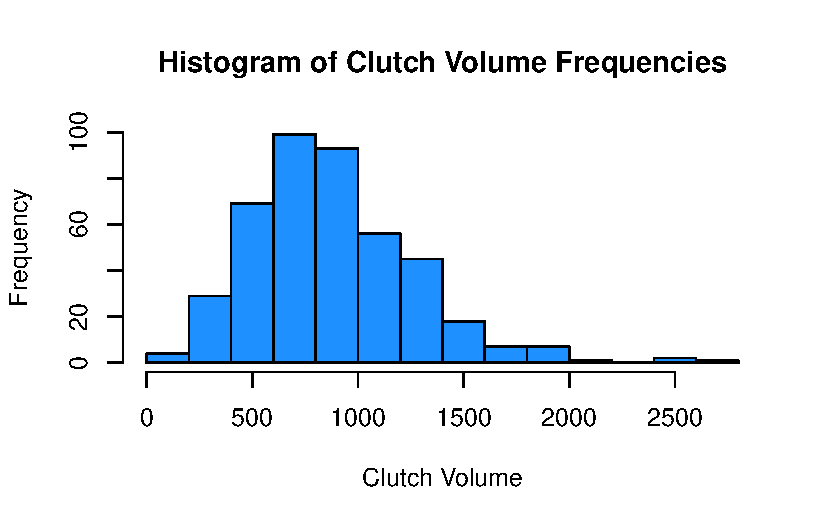
\includegraphics[width=\maxwidth]{figure/unnamed-chunk-51-1} 

}



\end{knitrout}

\subsection{Through Simulation}
The second method involves sampling randomly from the known normal distribution to simulate the probabilities that we drew directly in the above method.  In this case, the function \textit{rnorm} takes $n$ number of random samples from the normal distribution with the given mean and standard deviation.  In the \textit{hist} command, the specification that \textit{freq = FALSE} should be included to make the plot reflect percentages rather than frequency counts.  
\begin{knitrout}
\definecolor{shadecolor}{rgb}{0.969, 0.969, 0.969}\color{fgcolor}\begin{kframe}
\begin{alltt}
\hlkwd{set.seed}\hlstd{(}\hlnum{1}\hlstd{)}
\hlstd{x} \hlkwb{<-} \hlkwd{rnorm}\hlstd{(}\hlkwc{n} \hlstd{=} \hlnum{100000}\hlstd{,} \hlkwc{mean} \hlstd{=} \hlnum{0}\hlstd{,} \hlkwc{sd} \hlstd{=} \hlnum{1}\hlstd{)}
\hlkwd{hist}\hlstd{(x,} \hlkwc{breaks} \hlstd{=} \hlnum{100}\hlstd{,} \hlkwc{freq} \hlstd{=} \hlnum{FALSE}\hlstd{)}
\end{alltt}
\end{kframe}

{\centering 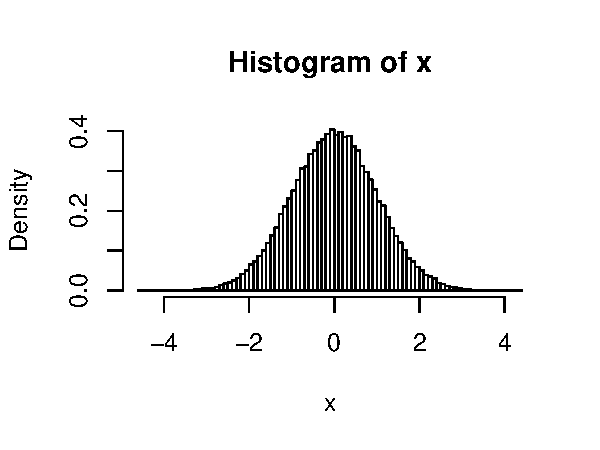
\includegraphics[width=\maxwidth]{figure/unnamed-chunk-52-1} 

}



\end{knitrout}

\subsection{A Comparison} 
Plotting both methods on the same graphs is useful for comparison as follows.  
\begin{knitrout}
\definecolor{shadecolor}{rgb}{0.969, 0.969, 0.969}\color{fgcolor}\begin{kframe}
\begin{alltt}
\hlkwd{hist}\hlstd{(x,} \hlkwc{freq} \hlstd{=} \hlnum{FALSE}\hlstd{,} \hlkwc{breaks} \hlstd{=} \hlnum{100}\hlstd{)}
\hlkwd{lines}\hlstd{(X,Y,} \hlkwc{col} \hlstd{=} \hlstr{"red"}\hlstd{)}
\end{alltt}
\end{kframe}

{\centering 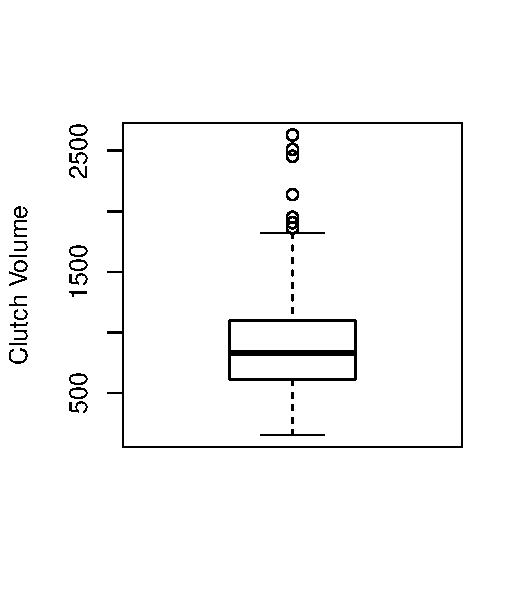
\includegraphics[width=\maxwidth]{figure/unnamed-chunk-53-1} 

}



\end{knitrout}

Note that the two show very similar results.  For practical purposes, \textit{dnorm} is typically used as it only requires one command and is the asymptotic result of simulations, rather than an approximation.  

\subsection{Probability Functions}
For the normal distribution, there are two more functions that are very useful, \textit{pnorm} and \textit{qnorm}. 

\subsubsection{pnorm} 
The function \textit{pnorm} tells the percentage of the normal distribution that is less than or equal to the value that is put in.  This corresponds to the gray area in the below plot and can be written as $pnorm(x, mean = \mu, sd = \sigma)$ which is equivalent to $P(X < x)$ where $X \sim N(\mu, \sigma)$ and $x$ is the point of interest.    
 
\begin{knitrout}
\definecolor{shadecolor}{rgb}{0.969, 0.969, 0.969}\color{fgcolor}

{\centering 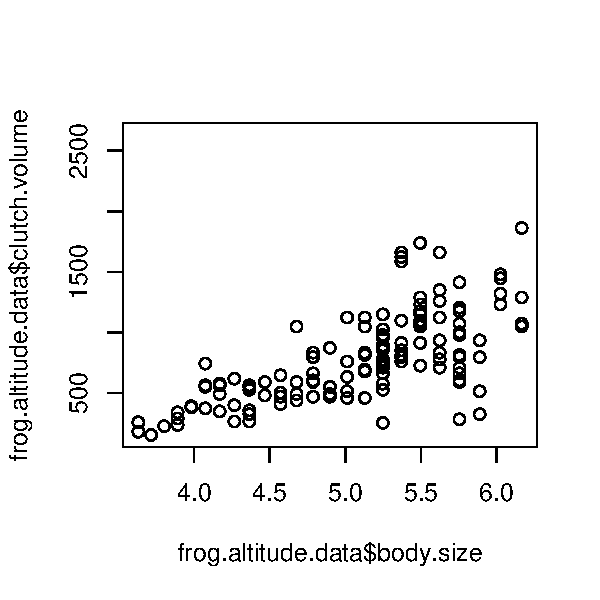
\includegraphics[width=\maxwidth]{figure/unnamed-chunk-54-1} 

}



\end{knitrout}

For some example scenarios, where the goal is to find a proportion of the normal distribution given $x$ or $z$, the following configurations of \textit{pnorm()} can be used: 
\begin{itemize}
\item $pnorm(z) = P(Z \leq z)$ 
\item $pnorm(z, lower.tail = FALSE) = P(Z > z)$ 
\item $pnorm(x, \mu, \sigma) = P(X \leq x)$ where $X = \sigma Z + \mu$ 
\item $pnorm(x, \mu, \sigma, lower.tail = FALSE) = P(X > x)$ where $X = \sigma Z + \mu$ 
\end{itemize}


\vspace{.75cm}
Several examples that are shown in the text can be evaluated as follows.  Keep note that for every question, there are multiple methods to arrive at the same answer.  The two main methods involve approximating to a standard normal distribution and allowing R to do all the work for you.  
\begin{knitrout}
\definecolor{shadecolor}{rgb}{0.969, 0.969, 0.969}\color{fgcolor}\begin{kframe}
\begin{alltt}
\hlcom{## Example 3.5}
\hlkwd{pnorm}\hlstd{(}\hlkwc{q} \hlstd{=} \hlnum{1}\hlstd{)}
\end{alltt}
\begin{verbatim}
## [1] 0.8413447
\end{verbatim}
\end{kframe}
\end{knitrout}

\begin{knitrout}
\definecolor{shadecolor}{rgb}{0.969, 0.969, 0.969}\color{fgcolor}\begin{kframe}
\begin{alltt}
\hlcom{## Example 3.7 }
\hlcom{# using the approximation to the standard normal }
\hlkwd{pnorm}\hlstd{(}\hlkwc{q} \hlstd{=} \hlnum{0.43}\hlstd{,} \hlkwc{lower.tail} \hlstd{=} \hlnum{FALSE}\hlstd{)}
\end{alltt}
\begin{verbatim}
## [1] 0.3335978
\end{verbatim}
\begin{alltt}
\hlnum{1} \hlopt{-} \hlkwd{pnorm}\hlstd{(}\hlkwc{q} \hlstd{=} \hlnum{0.43}\hlstd{)}
\end{alltt}
\begin{verbatim}
## [1] 0.3335978
\end{verbatim}
\begin{alltt}
\hlcom{# using the actual normal distribution }
\hlkwd{pnorm}\hlstd{(}\hlkwc{q} \hlstd{=} \hlnum{1630}\hlstd{,} \hlkwc{mean} \hlstd{=} \hlnum{1500}\hlstd{,} \hlkwc{sd} \hlstd{=} \hlnum{300}\hlstd{,} \hlkwc{lower.tail} \hlstd{=} \hlnum{FALSE}\hlstd{)}
\end{alltt}
\begin{verbatim}
## [1] 0.3323863
\end{verbatim}
\begin{alltt}
\hlnum{1} \hlopt{-} \hlkwd{pnorm}\hlstd{(}\hlkwc{q} \hlstd{=} \hlnum{1630}\hlstd{,} \hlkwc{mean} \hlstd{=} \hlnum{1500}\hlstd{,} \hlkwc{sd} \hlstd{=} \hlnum{300}\hlstd{)}
\end{alltt}
\begin{verbatim}
## [1] 0.3323863
\end{verbatim}
\end{kframe}
\end{knitrout}

\begin{knitrout}
\definecolor{shadecolor}{rgb}{0.969, 0.969, 0.969}\color{fgcolor}\begin{kframe}
\begin{alltt}
\hlcom{## Example 3.10 using standard normal approximation}
\hlkwd{pnorm}\hlstd{(}\hlnum{1.21}\hlstd{,} \hlkwc{lower.tail} \hlstd{=} \hlnum{TRUE}\hlstd{)} \hlopt{-} \hlkwd{pnorm}\hlstd{(}\hlopt{-}\hlnum{0.3}\hlstd{,} \hlkwc{lower.tail} \hlstd{=} \hlnum{TRUE}\hlstd{)}
\end{alltt}
\begin{verbatim}
## [1] 0.504772
\end{verbatim}
\begin{alltt}
\hlcom{# using actual distribution}
\hlkwd{pnorm}\hlstd{(}\hlkwc{q} \hlstd{=} \hlnum{74}\hlstd{,} \hlkwc{mean} \hlstd{=} \hlnum{70}\hlstd{,} \hlkwc{sd} \hlstd{=} \hlnum{3.3}\hlstd{,} \hlkwc{lower.tail} \hlstd{=} \hlnum{TRUE}\hlstd{)} \hlopt{-} \hlkwd{pnorm}\hlstd{(}\hlkwc{q} \hlstd{=} \hlnum{69}\hlstd{,} \hlkwc{mean} \hlstd{=} \hlnum{70}\hlstd{,}
    \hlkwc{sd} \hlstd{=} \hlnum{3.3}\hlstd{,} \hlkwc{lower.tail} \hlstd{=} \hlnum{TRUE}\hlstd{)}
\end{alltt}
\begin{verbatim}
## [1] 0.5063336
\end{verbatim}
\end{kframe}
\end{knitrout}


\subsubsection{qnorm} 
On the other hand, the \textit{qnorm} function is the inverse function, instead giving the $X$ value such that the given percentage of the distribution is less than or equal to that value. This function takes a known probability and returns a value on the normal distribution that is corresponding.  

Some sample configurations of using \textit{qnorm()} can be as follows,  
\begin{itemize}
\item $qnorm(p) = P(Z \leq z)$ 
\item $qnorm(p, lower.tail = FALSE) = P(Z > z)$ 
\item $qnorm(p, \mu, \sigma) = P(X \leq x)$ where $X = \sigma Z + \mu$ 
\item $qnorm(p, \mu, \sigma, lower.tail = FALSE) = P(X > x)$ where $X = \sigma Z + \mu$ 
\end{itemize}

\vspace{.5cm}
Working through an example in the main text, 
\begin{knitrout}
\definecolor{shadecolor}{rgb}{0.969, 0.969, 0.969}\color{fgcolor}\begin{kframe}
\begin{alltt}
\hlcom{## Example 3.12 }
\hlcom{# using standard normal }
\hlnum{70} \hlopt{+} \hlnum{3.3}\hlopt{*}\hlkwd{qnorm}\hlstd{(}\hlnum{0.4}\hlstd{)}
\end{alltt}
\begin{verbatim}
## [1] 69.16395
\end{verbatim}
\begin{alltt}
\hlcom{# one step function }
\hlkwd{qnorm}\hlstd{(}\hlkwc{p} \hlstd{=} \hlnum{.4}\hlstd{,} \hlkwc{mean} \hlstd{=} \hlnum{70}\hlstd{,} \hlkwc{sd} \hlstd{=} \hlnum{3.3}\hlstd{)}
\end{alltt}
\begin{verbatim}
## [1] 69.16395
\end{verbatim}
\end{kframe}
\end{knitrout}

\subsection{Evaluating the Normal Approximation} 
It is of interest to test the normality of a distriubtion in order to determine if approximation with a normal distribution is appropriate. There are two methods in $R$ that can be used to test this.  The first involves plotting the data with a histogram and then superimposing a line on top with the corresponding mean and standard deviation of the data.  The more closely that the histogram matches the line, the more appropriate a normal approximation would be.  

The second method utilizes the function \textit{qqnorm()}, which plots the residual differences between the observed data and the theoretical normal distribution that would match.  A line can be plotted on top of this plot, using \textit{qqline()}, which demonstrates how a perfect match would appear.  Deviation of the dots on the plot from the line shows lack of fit for the normal approimation.  

Both of these methods can be seen below in this recreation of \textit{Figure 3.10} from the main text.  The rows show the first and second methods respectively, while the columns show a progressively better fit to the normal from left to right.  
%%PUT THIS DATA INTO OIBIOSTAT PACKAGE 
\begin{knitrout}
\definecolor{shadecolor}{rgb}{0.969, 0.969, 0.969}\color{fgcolor}\begin{kframe}
\begin{alltt}
\hlstd{obs1} \hlkwb{<-} \hlkwd{c}\hlstd{(}\hlopt{-}\hlnum{0.01}\hlstd{,} \hlnum{1.39}\hlstd{,} \hlnum{1.598}\hlstd{,} \hlnum{0.383}\hlstd{,} \hlopt{-}\hlnum{0.084}\hlstd{,} \hlopt{-}\hlnum{0.475}\hlstd{,} \hlopt{-}\hlnum{0.105}\hlstd{,} \hlopt{-}\hlnum{1.062}\hlstd{,} \hlnum{0.607}\hlstd{,}
    \hlnum{0.539}\hlstd{,} \hlnum{0.871}\hlstd{,} \hlnum{0.45}\hlstd{,} \hlopt{-}\hlnum{0.039}\hlstd{,} \hlnum{1.256}\hlstd{,} \hlnum{0.55}\hlstd{,} \hlopt{-}\hlnum{0.333}\hlstd{,} \hlopt{-}\hlnum{0.252}\hlstd{,} \hlnum{1.187}\hlstd{,} \hlopt{-}\hlnum{0.916}\hlstd{,}
    \hlnum{0.677}\hlstd{,} \hlopt{-}\hlnum{1.324}\hlstd{,} \hlopt{-}\hlnum{1.773}\hlstd{,} \hlnum{1.813}\hlstd{,} \hlnum{0.023}\hlstd{,} \hlopt{-}\hlnum{2.291}\hlstd{,} \hlopt{-}\hlnum{1.361}\hlstd{,} \hlnum{0.642}\hlstd{,} \hlnum{0.249}\hlstd{,} \hlopt{-}\hlnum{0.132}\hlstd{,}
    \hlnum{1.345}\hlstd{,} \hlnum{0.629}\hlstd{,} \hlopt{-}\hlnum{1.274}\hlstd{,} \hlnum{0.435}\hlstd{,} \hlnum{0.043}\hlstd{,} \hlnum{0.55}\hlstd{,} \hlopt{-}\hlnum{0.465}\hlstd{,} \hlnum{0.756}\hlstd{,} \hlopt{-}\hlnum{0.396}\hlstd{,} \hlopt{-}\hlnum{0.767}\hlstd{,}
    \hlnum{1.348}\hlstd{)}

\hlstd{obs2} \hlkwb{<-} \hlkwd{c}\hlstd{(}\hlopt{-}\hlnum{0.78}\hlstd{,} \hlopt{-}\hlnum{0.552}\hlstd{,} \hlopt{-}\hlnum{0.027}\hlstd{,} \hlnum{0.33}\hlstd{,} \hlopt{-}\hlnum{0.964}\hlstd{,} \hlnum{0.865}\hlstd{,} \hlopt{-}\hlnum{0.112}\hlstd{,} \hlnum{0.075}\hlstd{,} \hlopt{-}\hlnum{0.392}\hlstd{,}
    \hlnum{0.365}\hlstd{,} \hlopt{-}\hlnum{1.738}\hlstd{,} \hlnum{0.491}\hlstd{,} \hlopt{-}\hlnum{0.245}\hlstd{,} \hlnum{0.436}\hlstd{,} \hlnum{0.016}\hlstd{,} \hlopt{-}\hlnum{0.202}\hlstd{,} \hlnum{1.322}\hlstd{,} \hlnum{0.515}\hlstd{,} \hlnum{0.333}\hlstd{,}
    \hlopt{-}\hlnum{0.28}\hlstd{,} \hlopt{-}\hlnum{0.843}\hlstd{,} \hlnum{0.181}\hlstd{,} \hlopt{-}\hlnum{0.284}\hlstd{,} \hlopt{-}\hlnum{0.409}\hlstd{,} \hlnum{0.542}\hlstd{,} \hlnum{0.117}\hlstd{,} \hlopt{-}\hlnum{0.194}\hlstd{,} \hlopt{-}\hlnum{0.415}\hlstd{,} \hlnum{1.362}\hlstd{,}
    \hlnum{0.826}\hlstd{,} \hlnum{1.099}\hlstd{,} \hlopt{-}\hlnum{1.243}\hlstd{,} \hlopt{-}\hlnum{0.265}\hlstd{,} \hlopt{-}\hlnum{0.387}\hlstd{,} \hlnum{0.901}\hlstd{,} \hlnum{0.706}\hlstd{,} \hlopt{-}\hlnum{0.353}\hlstd{,} \hlopt{-}\hlnum{1.05}\hlstd{,} \hlnum{0.081}\hlstd{,}
    \hlopt{-}\hlnum{1.102}\hlstd{,} \hlopt{-}\hlnum{2.705}\hlstd{,} \hlopt{-}\hlnum{0.142}\hlstd{,} \hlopt{-}\hlnum{0.608}\hlstd{,} \hlnum{0.661}\hlstd{,} \hlopt{-}\hlnum{0.616}\hlstd{,} \hlnum{1.025}\hlstd{,} \hlopt{-}\hlnum{1.384}\hlstd{,} \hlnum{0.337}\hlstd{,} \hlnum{1.14}\hlstd{,}
    \hlnum{0.523}\hlstd{,} \hlopt{-}\hlnum{0.662}\hlstd{,} \hlnum{0.19}\hlstd{,} \hlnum{1.468}\hlstd{,} \hlnum{2.38}\hlstd{,} \hlopt{-}\hlnum{0.351}\hlstd{,} \hlopt{-}\hlnum{2.125}\hlstd{,} \hlnum{1.141}\hlstd{,} \hlnum{1.149}\hlstd{,} \hlopt{-}\hlnum{0.448}\hlstd{,}
    \hlnum{1.166}\hlstd{,} \hlopt{-}\hlnum{0.269}\hlstd{,} \hlopt{-}\hlnum{0.145}\hlstd{,} \hlopt{-}\hlnum{1.319}\hlstd{,} \hlopt{-}\hlnum{0.445}\hlstd{,} \hlnum{0.34}\hlstd{,} \hlopt{-}\hlnum{1.789}\hlstd{,} \hlopt{-}\hlnum{0.626}\hlstd{,} \hlopt{-}\hlnum{1.302}\hlstd{,} \hlnum{2.441}\hlstd{,}
    \hlopt{-}\hlnum{2.016}\hlstd{,} \hlnum{0.333}\hlstd{,} \hlopt{-}\hlnum{0.019}\hlstd{,} \hlnum{0.457}\hlstd{,} \hlopt{-}\hlnum{0.706}\hlstd{,} \hlnum{0.236}\hlstd{,} \hlnum{0.496}\hlstd{,} \hlopt{-}\hlnum{0.02}\hlstd{,} \hlopt{-}\hlnum{0.228}\hlstd{,} \hlopt{-}\hlnum{1.756}\hlstd{,}
    \hlopt{-}\hlnum{1.309}\hlstd{,} \hlnum{0.564}\hlstd{,} \hlnum{1.597}\hlstd{,} \hlopt{-}\hlnum{0.172}\hlstd{,} \hlopt{-}\hlnum{0.369}\hlstd{,} \hlnum{0.478}\hlstd{,} \hlopt{-}\hlnum{0.854}\hlstd{,} \hlopt{-}\hlnum{0.52}\hlstd{,} \hlopt{-}\hlnum{0.045}\hlstd{,} \hlnum{1.654}\hlstd{,}
    \hlnum{1.122}\hlstd{,} \hlopt{-}\hlnum{0.155}\hlstd{,} \hlnum{0.281}\hlstd{,} \hlnum{0.205}\hlstd{,} \hlnum{0.096}\hlstd{,} \hlopt{-}\hlnum{2.303}\hlstd{,} \hlopt{-}\hlnum{1.399}\hlstd{,} \hlopt{-}\hlnum{0.877}\hlstd{,} \hlopt{-}\hlnum{1.205}\hlstd{,} \hlnum{0.02}\hlstd{,}
    \hlnum{0.563}\hlstd{)}

\hlstd{obs3} \hlkwb{<-} \hlkwd{c}\hlstd{(}\hlnum{0.673}\hlstd{,} \hlopt{-}\hlnum{0.538}\hlstd{,} \hlopt{-}\hlnum{0.703}\hlstd{,} \hlopt{-}\hlnum{0.004}\hlstd{,} \hlopt{-}\hlnum{1.395}\hlstd{,} \hlopt{-}\hlnum{0.354}\hlstd{,} \hlnum{0.415}\hlstd{,} \hlnum{1.097}\hlstd{,} \hlnum{0.74}\hlstd{,}
    \hlnum{0.657}\hlstd{,} \hlopt{-}\hlnum{0.759}\hlstd{,} \hlnum{0.415}\hlstd{,} \hlnum{2.094}\hlstd{,} \hlopt{-}\hlnum{0.662}\hlstd{,} \hlopt{-}\hlnum{0.161}\hlstd{,} \hlnum{0.293}\hlstd{,} \hlnum{0.057}\hlstd{,} \hlopt{-}\hlnum{1.487}\hlstd{,} \hlopt{-}\hlnum{1.822}\hlstd{,}
    \hlnum{1.192}\hlstd{,} \hlnum{2.186}\hlstd{,} \hlopt{-}\hlnum{0.26}\hlstd{,} \hlnum{0.453}\hlstd{,} \hlopt{-}\hlnum{0.267}\hlstd{,} \hlopt{-}\hlnum{0.049}\hlstd{,} \hlopt{-}\hlnum{1.075}\hlstd{,} \hlopt{-}\hlnum{0.959}\hlstd{,} \hlopt{-}\hlnum{2.338}\hlstd{,} \hlnum{0.512}\hlstd{,}
    \hlnum{2.365}\hlstd{,} \hlnum{0.56}\hlstd{,} \hlopt{-}\hlnum{0.812}\hlstd{,} \hlnum{0.363}\hlstd{,} \hlopt{-}\hlnum{0.731}\hlstd{,} \hlopt{-}\hlnum{0.644}\hlstd{,} \hlopt{-}\hlnum{0.448}\hlstd{,} \hlopt{-}\hlnum{0.024}\hlstd{,} \hlopt{-}\hlnum{0.024}\hlstd{,} \hlopt{-}\hlnum{1.133}\hlstd{,}
    \hlopt{-}\hlnum{0.692}\hlstd{,} \hlnum{1.233}\hlstd{,} \hlnum{0.566}\hlstd{,} \hlnum{1.109}\hlstd{,} \hlopt{-}\hlnum{2.215}\hlstd{,} \hlnum{0.494}\hlstd{,} \hlnum{0.011}\hlstd{,} \hlopt{-}\hlnum{2.785}\hlstd{,} \hlopt{-}\hlnum{0.59}\hlstd{,} \hlopt{-}\hlnum{0.895}\hlstd{,}
    \hlopt{-}\hlnum{1.084}\hlstd{,} \hlopt{-}\hlnum{0.848}\hlstd{,} \hlopt{-}\hlnum{0.129}\hlstd{,} \hlnum{1.132}\hlstd{,} \hlopt{-}\hlnum{0.851}\hlstd{,} \hlopt{-}\hlnum{0.419}\hlstd{,} \hlopt{-}\hlnum{0.232}\hlstd{,} \hlopt{-}\hlnum{0.789}\hlstd{,} \hlopt{-}\hlnum{2.018}\hlstd{,} \hlnum{1.302}\hlstd{,}
    \hlopt{-}\hlnum{1.276}\hlstd{,} \hlopt{-}\hlnum{0.592}\hlstd{,} \hlnum{1.578}\hlstd{,} \hlnum{0.474}\hlstd{,} \hlopt{-}\hlnum{0.437}\hlstd{,} \hlnum{0.3}\hlstd{,} \hlnum{0.145}\hlstd{,} \hlnum{0.263}\hlstd{,} \hlopt{-}\hlnum{2.189}\hlstd{,} \hlopt{-}\hlnum{0.265}\hlstd{,}
    \hlopt{-}\hlnum{0.02}\hlstd{,} \hlnum{0.85}\hlstd{,} \hlnum{1.523}\hlstd{,} \hlnum{0.938}\hlstd{,} \hlnum{0.651}\hlstd{,} \hlopt{-}\hlnum{1.866}\hlstd{,} \hlopt{-}\hlnum{2.202}\hlstd{,} \hlnum{0.083}\hlstd{,} \hlopt{-}\hlnum{0.816}\hlstd{,} \hlnum{1.082}\hlstd{,}
    \hlnum{1.448}\hlstd{,} \hlopt{-}\hlnum{1.563}\hlstd{,} \hlopt{-}\hlnum{0.145}\hlstd{,} \hlopt{-}\hlnum{1.168}\hlstd{,} \hlnum{1.633}\hlstd{,} \hlopt{-}\hlnum{0.472}\hlstd{,} \hlnum{0.173}\hlstd{,} \hlopt{-}\hlnum{1.592}\hlstd{,} \hlnum{0.623}\hlstd{,} \hlopt{-}\hlnum{0.674}\hlstd{,}
    \hlopt{-}\hlnum{1.336}\hlstd{,} \hlopt{-}\hlnum{0.059}\hlstd{,} \hlnum{0.209}\hlstd{,} \hlnum{0.152}\hlstd{,} \hlopt{-}\hlnum{0.345}\hlstd{,} \hlopt{-}\hlnum{0.686}\hlstd{,} \hlnum{2.494}\hlstd{,} \hlopt{-}\hlnum{0.616}\hlstd{,} \hlnum{0.615}\hlstd{,} \hlopt{-}\hlnum{0.718}\hlstd{,}
    \hlnum{1.748}\hlstd{,} \hlnum{0.011}\hlstd{,} \hlopt{-}\hlnum{0.936}\hlstd{,} \hlopt{-}\hlnum{0.196}\hlstd{,} \hlnum{0.839}\hlstd{,} \hlopt{-}\hlnum{0.099}\hlstd{,} \hlnum{0.216}\hlstd{,} \hlopt{-}\hlnum{0.036}\hlstd{,} \hlopt{-}\hlnum{0.687}\hlstd{,} \hlnum{1.126}\hlstd{,}
    \hlopt{-}\hlnum{0.024}\hlstd{,} \hlopt{-}\hlnum{0.239}\hlstd{,} \hlnum{1.475}\hlstd{,} \hlnum{1.548}\hlstd{,} \hlopt{-}\hlnum{1.254}\hlstd{,} \hlopt{-}\hlnum{1.513}\hlstd{,} \hlnum{0.635}\hlstd{,} \hlnum{0.482}\hlstd{,} \hlnum{1.068}\hlstd{,} \hlopt{-}\hlnum{0.814}\hlstd{,}
    \hlnum{1.171}\hlstd{,} \hlopt{-}\hlnum{0.509}\hlstd{,} \hlopt{-}\hlnum{0.733}\hlstd{,} \hlopt{-}\hlnum{0.32}\hlstd{,} \hlnum{0.05}\hlstd{,} \hlopt{-}\hlnum{0.359}\hlstd{,} \hlopt{-}\hlnum{0.22}\hlstd{,} \hlnum{0.269}\hlstd{,} \hlnum{1.581}\hlstd{,} \hlopt{-}\hlnum{0.967}\hlstd{,}
    \hlnum{1.725}\hlstd{,} \hlnum{0.322}\hlstd{,} \hlopt{-}\hlnum{0.176}\hlstd{,} \hlopt{-}\hlnum{0.655}\hlstd{,} \hlnum{2.362}\hlstd{,} \hlopt{-}\hlnum{0.004}\hlstd{,} \hlopt{-}\hlnum{1.209}\hlstd{,} \hlnum{0.622}\hlstd{,} \hlopt{-}\hlnum{1.125}\hlstd{,} \hlnum{1.767}\hlstd{,}
    \hlopt{-}\hlnum{0.053}\hlstd{,} \hlnum{0.066}\hlstd{,} \hlnum{0.049}\hlstd{,} \hlnum{0.45}\hlstd{,} \hlnum{0.302}\hlstd{,} \hlopt{-}\hlnum{0.172}\hlstd{,} \hlopt{-}\hlnum{1.237}\hlstd{,} \hlnum{0.072}\hlstd{,} \hlopt{-}\hlnum{1.007}\hlstd{,} \hlnum{0.312}\hlstd{,}
    \hlopt{-}\hlnum{0.647}\hlstd{,} \hlopt{-}\hlnum{0.759}\hlstd{,} \hlnum{0.753}\hlstd{,} \hlopt{-}\hlnum{1.179}\hlstd{,} \hlnum{0.984}\hlstd{,} \hlnum{1.947}\hlstd{,} \hlopt{-}\hlnum{0.653}\hlstd{,} \hlopt{-}\hlnum{0.34}\hlstd{,} \hlopt{-}\hlnum{0.669}\hlstd{,} \hlopt{-}\hlnum{0.066}\hlstd{,}
    \hlopt{-}\hlnum{1.774}\hlstd{,} \hlopt{-}\hlnum{1.409}\hlstd{,} \hlopt{-}\hlnum{0.875}\hlstd{,} \hlopt{-}\hlnum{0.225}\hlstd{,} \hlopt{-}\hlnum{0.775}\hlstd{,} \hlopt{-}\hlnum{0.657}\hlstd{,} \hlnum{0.812}\hlstd{,} \hlnum{2.278}\hlstd{,} \hlnum{0.25}\hlstd{,} \hlnum{1.206}\hlstd{,}
    \hlopt{-}\hlnum{0.646}\hlstd{,} \hlopt{-}\hlnum{0.693}\hlstd{,} \hlopt{-}\hlnum{0.545}\hlstd{,} \hlopt{-}\hlnum{1.44}\hlstd{,} \hlopt{-}\hlnum{1.548}\hlstd{,} \hlopt{-}\hlnum{0.924}\hlstd{,} \hlnum{0.408}\hlstd{,} \hlnum{1.135}\hlstd{,} \hlnum{1.173}\hlstd{,} \hlnum{1.472}\hlstd{,}
    \hlopt{-}\hlnum{0.578}\hlstd{,} \hlopt{-}\hlnum{0.04}\hlstd{,} \hlnum{0.422}\hlstd{,} \hlopt{-}\hlnum{0.214}\hlstd{,} \hlnum{0.983}\hlstd{,} \hlopt{-}\hlnum{1.605}\hlstd{,} \hlopt{-}\hlnum{0.6}\hlstd{,} \hlopt{-}\hlnum{0.641}\hlstd{,} \hlopt{-}\hlnum{0.501}\hlstd{,} \hlnum{0.795}\hlstd{,}
    \hlnum{0.542}\hlstd{,} \hlopt{-}\hlnum{1.471}\hlstd{,} \hlnum{0.185}\hlstd{,} \hlnum{0.504}\hlstd{,} \hlnum{3.559}\hlstd{,} \hlnum{0.487}\hlstd{,} \hlnum{0.406}\hlstd{,} \hlnum{0.318}\hlstd{,} \hlnum{1.485}\hlstd{,} \hlnum{0.217}\hlstd{,} \hlnum{0.409}\hlstd{,}
    \hlopt{-}\hlnum{0.005}\hlstd{,} \hlopt{-}\hlnum{0.351}\hlstd{,} \hlopt{-}\hlnum{0.932}\hlstd{,} \hlnum{1.504}\hlstd{,} \hlnum{0.528}\hlstd{,} \hlopt{-}\hlnum{2.061}\hlstd{,} \hlopt{-}\hlnum{1.405}\hlstd{,} \hlopt{-}\hlnum{0.256}\hlstd{,} \hlnum{2.293}\hlstd{,} \hlnum{0.385}\hlstd{,}
    \hlnum{0.363}\hlstd{,} \hlnum{0.928}\hlstd{,} \hlnum{1.455}\hlstd{,} \hlopt{-}\hlnum{0.317}\hlstd{,} \hlnum{0.804}\hlstd{,} \hlopt{-}\hlnum{1.358}\hlstd{,} \hlnum{1.137}\hlstd{,} \hlopt{-}\hlnum{1.072}\hlstd{,} \hlnum{0.015}\hlstd{,} \hlopt{-}\hlnum{0.905}\hlstd{,}
    \hlnum{1.768}\hlstd{,} \hlopt{-}\hlnum{0.562}\hlstd{,} \hlopt{-}\hlnum{1.268}\hlstd{,} \hlnum{0.284}\hlstd{,} \hlopt{-}\hlnum{0.952}\hlstd{,} \hlopt{-}\hlnum{1.163}\hlstd{,} \hlopt{-}\hlnum{0.352}\hlstd{,} \hlnum{0.507}\hlstd{,} \hlnum{0.194}\hlstd{,} \hlnum{0.579}\hlstd{,}
    \hlnum{0.345}\hlstd{,} \hlnum{1.171}\hlstd{,} \hlopt{-}\hlnum{1.009}\hlstd{,} \hlnum{0.622}\hlstd{,} \hlopt{-}\hlnum{1.311}\hlstd{,} \hlnum{0.407}\hlstd{,} \hlnum{0.277}\hlstd{,} \hlopt{-}\hlnum{0.191}\hlstd{,} \hlopt{-}\hlnum{1.417}\hlstd{,} \hlnum{0.089}\hlstd{,}
    \hlopt{-}\hlnum{1.607}\hlstd{,} \hlnum{0.012}\hlstd{,} \hlopt{-}\hlnum{1.355}\hlstd{,} \hlnum{0.267}\hlstd{,} \hlnum{2.723}\hlstd{,} \hlopt{-}\hlnum{1.16}\hlstd{,} \hlopt{-}\hlnum{2.613}\hlstd{,} \hlnum{0.161}\hlstd{,} \hlopt{-}\hlnum{0.371}\hlstd{,} \hlopt{-}\hlnum{0.331}\hlstd{,}
    \hlnum{0.726}\hlstd{,} \hlnum{1.389}\hlstd{,} \hlnum{1.111}\hlstd{,} \hlopt{-}\hlnum{0.911}\hlstd{,} \hlopt{-}\hlnum{0.74}\hlstd{,} \hlopt{-}\hlnum{0.818}\hlstd{,} \hlnum{1.667}\hlstd{,} \hlnum{0.714}\hlstd{,} \hlopt{-}\hlnum{0.262}\hlstd{,} \hlnum{0.045}\hlstd{,}
    \hlnum{0.009}\hlstd{,} \hlopt{-}\hlnum{0.022}\hlstd{,} \hlopt{-}\hlnum{0.508}\hlstd{,} \hlopt{-}\hlnum{1.423}\hlstd{,} \hlnum{0.229}\hlstd{,} \hlnum{0.765}\hlstd{,} \hlopt{-}\hlnum{0.549}\hlstd{,} \hlnum{0.587}\hlstd{,} \hlnum{0.183}\hlstd{,} \hlopt{-}\hlnum{0.091}\hlstd{,}
    \hlnum{0.501}\hlstd{,} \hlnum{0.452}\hlstd{,} \hlnum{1.927}\hlstd{,} \hlopt{-}\hlnum{0.237}\hlstd{,} \hlnum{0.697}\hlstd{,} \hlnum{0.181}\hlstd{,} \hlopt{-}\hlnum{1.044}\hlstd{,} \hlnum{0.605}\hlstd{,} \hlnum{1.178}\hlstd{,} \hlnum{1.047}\hlstd{,}
    \hlnum{1.405}\hlstd{,} \hlnum{1.686}\hlstd{,} \hlopt{-}\hlnum{0.382}\hlstd{,} \hlnum{1.217}\hlstd{,} \hlnum{0.499}\hlstd{,} \hlnum{0.271}\hlstd{,} \hlnum{0.662}\hlstd{,} \hlnum{0.562}\hlstd{,} \hlnum{0.528}\hlstd{,} \hlnum{0.684}\hlstd{,} \hlopt{-}\hlnum{0.751}\hlstd{,}
    \hlnum{1.843}\hlstd{,} \hlnum{1.063}\hlstd{,} \hlopt{-}\hlnum{1.828}\hlstd{,} \hlnum{1.345}\hlstd{,} \hlnum{0.077}\hlstd{,} \hlnum{0.943}\hlstd{,} \hlnum{1.048}\hlstd{,} \hlnum{1.637}\hlstd{,} \hlopt{-}\hlnum{0.535}\hlstd{,} \hlnum{0.664}\hlstd{,}
    \hlnum{0.433}\hlstd{,} \hlopt{-}\hlnum{0.559}\hlstd{,} \hlopt{-}\hlnum{0.141}\hlstd{,} \hlnum{0.663}\hlstd{,} \hlnum{0.777}\hlstd{,} \hlnum{1.442}\hlstd{,} \hlopt{-}\hlnum{0.685}\hlstd{,} \hlopt{-}\hlnum{0.451}\hlstd{,} \hlnum{0.265}\hlstd{,} \hlnum{0.727}\hlstd{,}
    \hlopt{-}\hlnum{1.206}\hlstd{,} \hlnum{0.339}\hlstd{,} \hlopt{-}\hlnum{0.32}\hlstd{,} \hlnum{0.079}\hlstd{,} \hlopt{-}\hlnum{0.052}\hlstd{,} \hlnum{0.097}\hlstd{,} \hlnum{0.827}\hlstd{,} \hlopt{-}\hlnum{2.121}\hlstd{,} \hlnum{0.57}\hlstd{,} \hlopt{-}\hlnum{2.563}\hlstd{,}
    \hlnum{0.663}\hlstd{,} \hlopt{-}\hlnum{1.115}\hlstd{,} \hlnum{0.176}\hlstd{,} \hlnum{0.786}\hlstd{,} \hlnum{0.783}\hlstd{,} \hlnum{1.068}\hlstd{,} \hlopt{-}\hlnum{1.734}\hlstd{,} \hlnum{1.255}\hlstd{,} \hlnum{0.79}\hlstd{,} \hlopt{-}\hlnum{0.721}\hlstd{,}
    \hlopt{-}\hlnum{0.028}\hlstd{,} \hlnum{0.514}\hlstd{,} \hlopt{-}\hlnum{0.963}\hlstd{,} \hlopt{-}\hlnum{2.052}\hlstd{,} \hlopt{-}\hlnum{1.195}\hlstd{,} \hlnum{0.091}\hlstd{,} \hlnum{0.187}\hlstd{,} \hlnum{0.61}\hlstd{,} \hlopt{-}\hlnum{1.61}\hlstd{,} \hlopt{-}\hlnum{0.066}\hlstd{,}
    \hlnum{2.733}\hlstd{,} \hlopt{-}\hlnum{0.853}\hlstd{,} \hlopt{-}\hlnum{1.175}\hlstd{,} \hlnum{1.079}\hlstd{,} \hlopt{-}\hlnum{0.58}\hlstd{,} \hlnum{0.033}\hlstd{,} \hlnum{1.213}\hlstd{,} \hlnum{0.367}\hlstd{,} \hlopt{-}\hlnum{0.567}\hlstd{,} \hlopt{-}\hlnum{0.107}\hlstd{,}
    \hlnum{0.188}\hlstd{,} \hlopt{-}\hlnum{0.091}\hlstd{,} \hlopt{-}\hlnum{0.932}\hlstd{,} \hlopt{-}\hlnum{0.11}\hlstd{,} \hlopt{-}\hlnum{1.312}\hlstd{,} \hlnum{0.968}\hlstd{,} \hlnum{0.698}\hlstd{,} \hlnum{1.089}\hlstd{,} \hlnum{0.695}\hlstd{,} \hlnum{1.309}\hlstd{,}
    \hlnum{1.017}\hlstd{,} \hlnum{0.677}\hlstd{,} \hlnum{0.471}\hlstd{,} \hlopt{-}\hlnum{1.524}\hlstd{,} \hlopt{-}\hlnum{1.82}\hlstd{,} \hlnum{0.256}\hlstd{,} \hlnum{0.397}\hlstd{,} \hlopt{-}\hlnum{0.489}\hlstd{,} \hlnum{1.734}\hlstd{,} \hlopt{-}\hlnum{0.297}\hlstd{,}
    \hlnum{0.075}\hlstd{,} \hlnum{0.533}\hlstd{,} \hlnum{0.165}\hlstd{,} \hlnum{0.814}\hlstd{,} \hlopt{-}\hlnum{1.915}\hlstd{,} \hlopt{-}\hlnum{0.332}\hlstd{,} \hlnum{1.035}\hlstd{,} \hlopt{-}\hlnum{0.858}\hlstd{,} \hlnum{1.07}\hlstd{,} \hlnum{0.532}\hlstd{,}
    \hlopt{-}\hlnum{0.016}\hlstd{,} \hlnum{1.932}\hlstd{,} \hlopt{-}\hlnum{0.564}\hlstd{,} \hlopt{-}\hlnum{0.018}\hlstd{,} \hlopt{-}\hlnum{0.542}\hlstd{,} \hlnum{1.048}\hlstd{,} \hlnum{0.759}\hlstd{,} \hlnum{1.575}\hlstd{,} \hlopt{-}\hlnum{1.263}\hlstd{,} \hlopt{-}\hlnum{0.667}\hlstd{,}
    \hlopt{-}\hlnum{1.195}\hlstd{,} \hlopt{-}\hlnum{0.179}\hlstd{,} \hlnum{0.337}\hlstd{,} \hlnum{0.257}\hlstd{,} \hlnum{0.356}\hlstd{,} \hlnum{0.375}\hlstd{,} \hlopt{-}\hlnum{1.326}\hlstd{,} \hlnum{0.509}\hlstd{,} \hlnum{0.975}\hlstd{)}

\hlkwd{par}\hlstd{(}\hlkwc{mfrow} \hlstd{=} \hlkwd{c}\hlstd{(}\hlnum{2}\hlstd{,} \hlnum{3}\hlstd{))}

\hlkwd{hist}\hlstd{(obs1,} \hlkwc{breaks} \hlstd{=} \hlnum{12}\hlstd{,} \hlkwc{xlim} \hlstd{=} \hlkwd{c}\hlstd{(}\hlopt{-}\hlnum{3}\hlstd{,} \hlnum{3}\hlstd{),} \hlkwc{freq} \hlstd{=} \hlnum{FALSE}\hlstd{,} \hlkwc{col} \hlstd{=} \hlstr{"light blue"}\hlstd{,} \hlkwc{main} \hlstd{=} \hlstr{" "}\hlstd{)}
\hlstd{x1} \hlkwb{<-} \hlkwd{seq}\hlstd{(}\hlkwd{min}\hlstd{(obs1)} \hlopt{-} \hlnum{2}\hlstd{,} \hlkwd{max}\hlstd{(obs1)} \hlopt{+} \hlnum{2}\hlstd{,} \hlnum{0.01}\hlstd{)}
\hlstd{y1} \hlkwb{<-} \hlkwd{dnorm}\hlstd{(x1,} \hlkwd{mean}\hlstd{(obs1),} \hlkwd{sd}\hlstd{(obs1))}
\hlkwd{lines}\hlstd{(x1, y1,} \hlkwc{lwd} \hlstd{=} \hlnum{1.5}\hlstd{)}

\hlkwd{hist}\hlstd{(obs2,} \hlkwc{breaks} \hlstd{=} \hlnum{12}\hlstd{,} \hlkwc{xlim} \hlstd{=} \hlkwd{c}\hlstd{(}\hlopt{-}\hlnum{3}\hlstd{,} \hlnum{3}\hlstd{),} \hlkwc{freq} \hlstd{=} \hlnum{FALSE}\hlstd{,} \hlkwc{col} \hlstd{=} \hlstr{"light green"}\hlstd{,}
    \hlkwc{main} \hlstd{=} \hlstr{" "}\hlstd{)}
\hlstd{x2} \hlkwb{<-} \hlkwd{seq}\hlstd{(}\hlkwd{min}\hlstd{(obs2)} \hlopt{-} \hlnum{2}\hlstd{,} \hlkwd{max}\hlstd{(obs2)} \hlopt{+} \hlnum{2}\hlstd{,} \hlnum{0.01}\hlstd{)}
\hlstd{y2} \hlkwb{<-} \hlkwd{dnorm}\hlstd{(x2,} \hlkwd{mean}\hlstd{(obs2),} \hlkwd{sd}\hlstd{(obs2))}
\hlkwd{lines}\hlstd{(x2, y2,} \hlkwc{lwd} \hlstd{=} \hlnum{1.5}\hlstd{)}

\hlkwd{hist}\hlstd{(obs3,} \hlkwc{breaks} \hlstd{=} \hlnum{12}\hlstd{,} \hlkwc{xlim} \hlstd{=} \hlkwd{c}\hlstd{(}\hlopt{-}\hlnum{3}\hlstd{,} \hlnum{3}\hlstd{),} \hlkwc{freq} \hlstd{=} \hlnum{FALSE}\hlstd{,} \hlkwc{col} \hlstd{=} \hlstr{"yellow"}\hlstd{,} \hlkwc{main} \hlstd{=} \hlstr{" "}\hlstd{)}
\hlstd{x3} \hlkwb{<-} \hlkwd{seq}\hlstd{(}\hlkwd{min}\hlstd{(obs3)} \hlopt{-} \hlnum{2}\hlstd{,} \hlkwd{max}\hlstd{(obs3)} \hlopt{+} \hlnum{2}\hlstd{,} \hlnum{0.01}\hlstd{)}
\hlstd{y3} \hlkwb{<-} \hlkwd{dnorm}\hlstd{(x3,} \hlkwd{mean}\hlstd{(obs3),} \hlkwd{sd}\hlstd{(obs3))}
\hlkwd{lines}\hlstd{(x3, y3,} \hlkwc{lwd} \hlstd{=} \hlnum{1.5}\hlstd{)}

\hlkwd{qqnorm}\hlstd{(obs1,} \hlkwc{col} \hlstd{=} \hlstr{"light blue"}\hlstd{,} \hlkwc{main} \hlstd{=} \hlstr{" "}\hlstd{)}
\hlkwd{qqline}\hlstd{(obs1)}

\hlkwd{qqnorm}\hlstd{(obs2,} \hlkwc{col} \hlstd{=} \hlstr{"light green"}\hlstd{,} \hlkwc{main} \hlstd{=} \hlstr{" "}\hlstd{)}
\hlkwd{qqline}\hlstd{(obs2)}

\hlkwd{qqnorm}\hlstd{(obs3,} \hlkwc{col} \hlstd{=} \hlstr{"yellow"}\hlstd{,} \hlkwc{main} \hlstd{=} \hlstr{" "}\hlstd{)}
\hlkwd{qqline}\hlstd{(obs3)}
\end{alltt}
\end{kframe}

{\centering 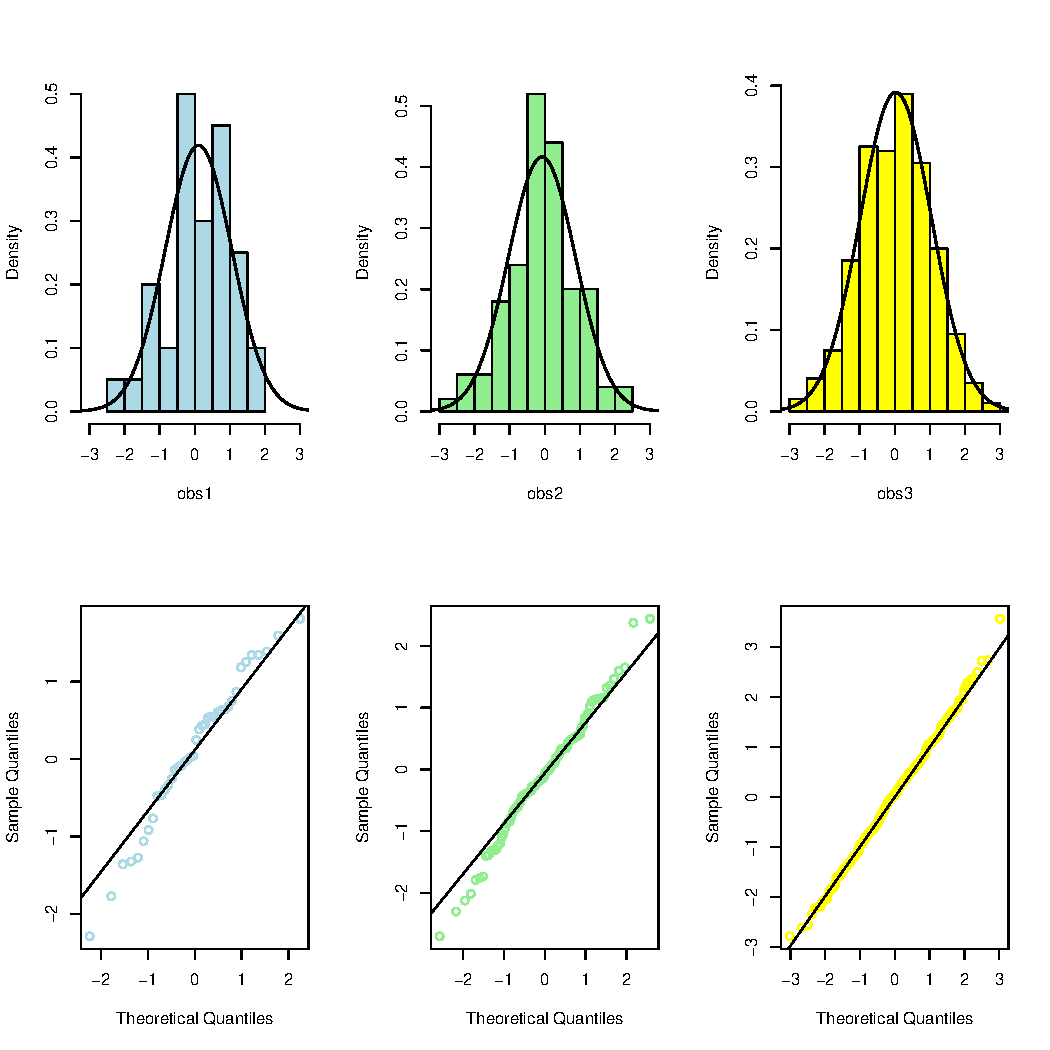
\includegraphics[width=\maxwidth]{figure/unnamed-chunk-59-1} 

}



\end{knitrout}



\begin{knitrout}
\definecolor{shadecolor}{rgb}{0.969, 0.969, 0.969}\color{fgcolor}\begin{kframe}
\begin{alltt}
\hlkwd{par}\hlstd{(}\hlkwc{mfrow} \hlstd{=} \hlkwd{c}\hlstd{(}\hlnum{1}\hlstd{,} \hlnum{2}\hlstd{))}
\hlstd{obs} \hlkwb{<-} \hlkwd{c}\hlstd{(}\hlopt{-}\hlnum{110}\hlstd{,} \hlopt{-}\hlnum{9}\hlstd{,} \hlopt{-}\hlnum{60}\hlstd{,} \hlnum{316}\hlstd{,} \hlopt{-}\hlnum{200}\hlstd{,} \hlopt{-}\hlnum{196}\hlstd{,} \hlnum{320}\hlstd{,} \hlopt{-}\hlnum{160}\hlstd{,} \hlnum{31}\hlstd{,} \hlnum{331}\hlstd{,} \hlnum{1731}\hlstd{,} \hlnum{21}\hlstd{,} \hlopt{-}\hlnum{926}\hlstd{,}
    \hlopt{-}\hlnum{475}\hlstd{,} \hlnum{914}\hlstd{,} \hlopt{-}\hlnum{300}\hlstd{,} \hlopt{-}\hlnum{15}\hlstd{,} \hlnum{1}\hlstd{,} \hlopt{-}\hlnum{29}\hlstd{,} \hlnum{829}\hlstd{,} \hlnum{761}\hlstd{,} \hlnum{227}\hlstd{,} \hlopt{-}\hlnum{141}\hlstd{,} \hlopt{-}\hlnum{672}\hlstd{,} \hlnum{352}\hlstd{,} \hlnum{385}\hlstd{,} \hlnum{24}\hlstd{,} \hlnum{103}\hlstd{,}
    \hlopt{-}\hlnum{826}\hlstd{,} \hlnum{95}\hlstd{,} \hlnum{115}\hlstd{,} \hlnum{39}\hlstd{,} \hlopt{-}\hlnum{9}\hlstd{,} \hlopt{-}\hlnum{1000}\hlstd{,} \hlopt{-}\hlnum{35}\hlstd{,} \hlopt{-}\hlnum{200}\hlstd{,} \hlopt{-}\hlnum{200}\hlstd{,} \hlnum{235}\hlstd{,} \hlnum{70}\hlstd{,} \hlnum{307}\hlstd{,} \hlnum{135}\hlstd{,} \hlnum{60}\hlstd{,} \hlopt{-}\hlnum{100}\hlstd{,}
    \hlopt{-}\hlnum{295}\hlstd{,} \hlopt{-}\hlnum{1000}\hlstd{,} \hlnum{361}\hlstd{,} \hlopt{-}\hlnum{95}\hlstd{,} \hlnum{337}\hlstd{,} \hlnum{3712}\hlstd{,} \hlopt{-}\hlnum{255}\hlstd{)}

\hlstd{x} \hlkwb{<-} \hlkwd{seq}\hlstd{(}\hlkwd{min}\hlstd{(obs)} \hlopt{-} \hlnum{3000}\hlstd{,} \hlkwd{max}\hlstd{(obs)} \hlopt{+} \hlnum{3000}\hlstd{,} \hlnum{1}\hlstd{)}
\hlstd{y} \hlkwb{<-} \hlkwd{dnorm}\hlstd{(x,} \hlkwd{mean}\hlstd{(obs),} \hlkwd{sd}\hlstd{(obs))}

\hlkwd{hist}\hlstd{(obs,} \hlkwc{freq} \hlstd{=} \hlnum{FALSE}\hlstd{)}
\hlkwd{lines}\hlstd{(x, y)}

\hlkwd{qqnorm}\hlstd{(obs)}
\hlkwd{qqline}\hlstd{(obs)}
\end{alltt}
\end{kframe}

{\centering 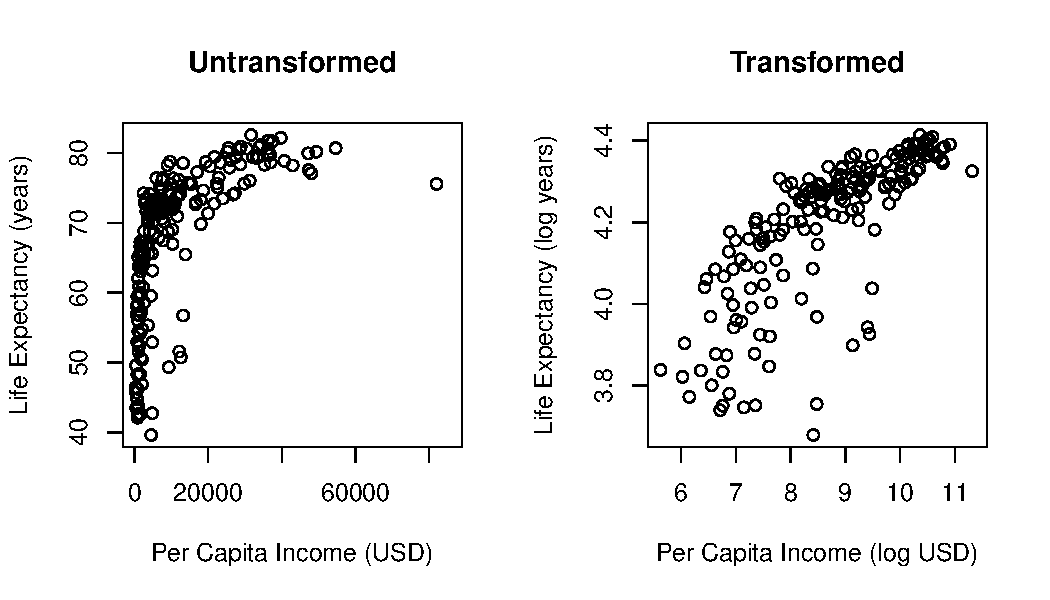
\includegraphics[width=\maxwidth]{figure/unnamed-chunk-60-1} 

}



\end{knitrout}

\section{Evaluating the Normal Distribution}
%%% COME FILL THIS IN -- A LOT OF THIS IS WRITTEN OUT IN CHAPTER 6 WITH CONTEXT (is it better there??)

\section{Binomial Distribution}
A random variable which follows a \textbf{binomial distribution} can be written as
\[ X \sim Binom(n,p) \]
where $n$ represents the sample size and $p$ represents the probability of success.  

The functions seen above for the normal distribution can be similarly used for the binomial as follows where the necessary arguments are \textit{size} and \textit{prob}, corresponding respectively to $n$ and $p$ in our above representation of the binomial.
\begin{itemize} 
\item \textit{dbinom}
\item \textit{rbinom}
\item \textit{pbinom}
\item \textit{qbinom}
\end{itemize}

Similar to the above example with the normal distribution, these functions can be used in multiple ways to work with the binomial distribution.  

\subsection{Accessing the Binomial Distribution}
As above, the binomial distribution can be accessed directly with \textit{dbinom} as follows: 
\begin{knitrout}
\definecolor{shadecolor}{rgb}{0.969, 0.969, 0.969}\color{fgcolor}\begin{kframe}
\begin{alltt}
\hlcom{## Splitting the graphics window into two panes }
\hlkwd{par}\hlstd{(}\hlkwc{mfrow}\hlstd{=}\hlkwd{c}\hlstd{(}\hlnum{1}\hlstd{,}\hlnum{2}\hlstd{))}
\hlcom{## Directly plotting the binomial distribution}
 \hlcom{# getting a list of values to evaluate distribution}
\hlstd{X} \hlkwb{=} \hlkwd{seq}\hlstd{(}\hlnum{0}\hlstd{,} \hlnum{10}\hlstd{,} \hlnum{1}\hlstd{)}
 \hlcom{# getting normal distribution value of the given X values }
\hlstd{Y} \hlkwb{=} \hlkwd{dbinom}\hlstd{(X,} \hlkwc{size} \hlstd{=} \hlnum{10}\hlstd{,} \hlkwc{prob} \hlstd{=} \hlnum{.25}\hlstd{)}
 \hlcom{# plotting results }
\hlkwd{plot}\hlstd{(X,Y,} \hlkwc{type} \hlstd{=} \hlstr{"s"}\hlstd{,} \hlkwc{main} \hlstd{=} \hlstr{"Direct Plot"}\hlstd{,} \hlkwc{xlim} \hlstd{=} \hlkwd{c}\hlstd{(}\hlnum{0}\hlstd{,}\hlnum{10}\hlstd{))}

\hlcom{## Instead Using Simulation}
\hlkwd{set.seed}\hlstd{(}\hlnum{1}\hlstd{)}
\hlstd{x} \hlkwb{<-} \hlkwd{rbinom}\hlstd{(}\hlkwc{n} \hlstd{=} \hlnum{100000}\hlstd{,} \hlkwc{size} \hlstd{=} \hlnum{10}\hlstd{,} \hlkwc{prob} \hlstd{=} \hlnum{.25}\hlstd{)}
\hlkwd{hist}\hlstd{(x,} \hlkwc{breaks} \hlstd{=} \hlnum{10}\hlstd{,} \hlkwc{freq} \hlstd{=} \hlnum{FALSE}\hlstd{,}\hlkwc{right} \hlstd{=} \hlnum{FALSE}\hlstd{,} \hlkwc{main} \hlstd{=} \hlstr{"Simulation"}\hlstd{,} \hlkwc{xlim} \hlstd{=} \hlkwd{c}\hlstd{(}\hlnum{0}\hlstd{,}\hlnum{10}\hlstd{))}
\hlkwd{box}\hlstd{()}
\end{alltt}
\end{kframe}

{\centering 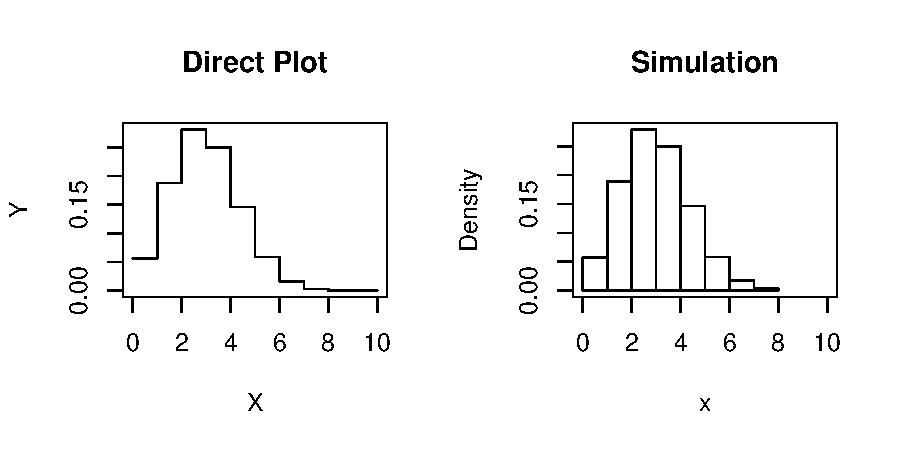
\includegraphics[width=\maxwidth]{figure/unnamed-chunk-61-1} 

}



\end{knitrout}

\subsection{Comparison of the Methods}
Superimposing the graphs is another useful mechanism for direct comparison of the two methods. 
\begin{knitrout}
\definecolor{shadecolor}{rgb}{0.969, 0.969, 0.969}\color{fgcolor}\begin{kframe}
\begin{alltt}
\hlkwd{hist}\hlstd{(x,} \hlkwc{breaks} \hlstd{=} \hlnum{10}\hlstd{,} \hlkwc{freq} \hlstd{=} \hlnum{FALSE}\hlstd{,}\hlkwc{right} \hlstd{=} \hlnum{FALSE}\hlstd{)}
\hlkwd{lines}\hlstd{(X,Y,} \hlkwc{type} \hlstd{=} \hlstr{"s"}\hlstd{,} \hlkwc{col} \hlstd{=} \hlstr{"red"}\hlstd{)}
\end{alltt}
\end{kframe}

{\centering 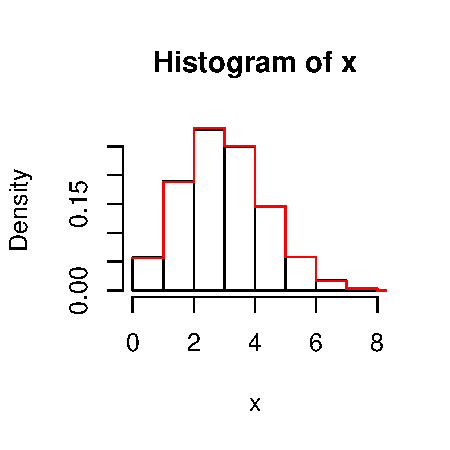
\includegraphics[width=\maxwidth]{figure/unnamed-chunk-62-1} 

}



\end{knitrout}

\subsection{Continuous and Discrete Distributions}
Using the binomial distribution highlights an important feature of distributions that must be considered: whether the random variable is \textbf{discrete} or \textbf{continuous}.  A discrete distribution can only take on specified values, typically the integers. The binomial is a great example of this - it can be any integer greater than or equal to zero.  For example, the possible values of a binomial are \{0, 1, 2, 3, ...\}.  

On the other hand, a continuous distribution can take on any real number within a specified range.  For example, looking at the standard normal distribution, a list of some possible values could be \{0, 0.1, 0.01, 0.001, 0.0001, ...\}.  This is a limited list of the infinite list of possible values that a continuous distribution could take on.  

The reason we care about the classification of a random variable as discrete or continous is that it affects the implementation of probability functions in $R$.  Let's walk through an example to see the difference.  Consider a normally distributed random variable, $X$, and a binomially distributed random variable, $Y$. 
\[ X \sim N(0,1) \; \; \; \; \; \; \; \; \; \; \; \;  Y \sim Binom(15,0.5) \]
If the goal is to determine the probability of being less than 2 for each of these two distributions, this would be equivalent to $P(X < 2)$ and $P(Y < 2)$.  However, for the binomial distribution $P(Y<2) = P(Y \leq 1) = P(Y=0) + P(Y=1)$ because there is a discrete set of possible values that $Y$ can take on.  $Y$ can only take on the integer values, and less than 2, that just leaves 0 and 1, whereas the normal distribution can take on any non-integer value in that interval, which is an infinite number of values.  For the normal distribution, solving for $P(Y<2)$ is mathematically equivalent to $P(Y \leq 2)$ because it is continuous.  

To solve for these probabilities, use \textit{pnorm} and \textit{pbinom}, noting that for the discrete binomial case, these functions automatically give the less than or equal to probability, not just the less than probability.  The correct commands can be seen through the following examples from the text. 
\subsection{Examples of the Binomial}
\vspace{0.5cm}
To summarize, the binomial probaility functions can be used as follows, 
\begin{itemize} 
\item $dbinom(x,n,p) = P(X = x)$ 
\item $pbinom(x,n,p) = P(X \leq x)$ 
\item $pbinom(x,n,p, lower.tail = FALSE) = P(X > x)$ 
\end{itemize} 

\begin{knitrout}
\definecolor{shadecolor}{rgb}{0.969, 0.969, 0.969}\color{fgcolor}\begin{kframe}
\begin{alltt}
\hlcom{## Example 3.19 }
\hlkwd{dbinom}\hlstd{(}\hlnum{1}\hlstd{,} \hlkwc{size} \hlstd{=} \hlnum{4}\hlstd{,} \hlkwc{prob} \hlstd{=} \hlnum{0.35}\hlstd{)}
\end{alltt}
\begin{verbatim}
## [1] 0.384475
\end{verbatim}
\end{kframe}
\end{knitrout}

\begin{knitrout}
\definecolor{shadecolor}{rgb}{0.969, 0.969, 0.969}\color{fgcolor}\begin{kframe}
\begin{alltt}
\hlcom{## Example 3.23}
\hlkwd{dbinom}\hlstd{(}\hlnum{3}\hlstd{,} \hlkwc{size} \hlstd{=} \hlnum{8}\hlstd{,} \hlkwc{prob} \hlstd{=} \hlnum{0.35}\hlstd{)}
\end{alltt}
\begin{verbatim}
## [1] 0.2785858
\end{verbatim}
\end{kframe}
\end{knitrout}

\begin{knitrout}
\definecolor{shadecolor}{rgb}{0.969, 0.969, 0.969}\color{fgcolor}\begin{kframe}
\begin{alltt}
\hlcom{## Example 3.24}
\hlkwd{pbinom}\hlstd{(}\hlnum{3}\hlstd{,} \hlkwc{size} \hlstd{=} \hlnum{8}\hlstd{,} \hlkwc{prob} \hlstd{=} \hlnum{0.35}\hlstd{,} \hlkwc{lower.tail} \hlstd{=} \hlnum{TRUE}\hlstd{)}
\end{alltt}
\begin{verbatim}
## [1] 0.7063994
\end{verbatim}
\end{kframe}
\end{knitrout}

\begin{knitrout}
\definecolor{shadecolor}{rgb}{0.969, 0.969, 0.969}\color{fgcolor}\begin{kframe}
\begin{alltt}
\hlcom{## Example 3.27 }
\hlkwd{pnorm}\hlstd{(}\hlnum{59}\hlstd{,} \hlkwc{mean} \hlstd{= (}\hlnum{400}\hlopt{*}\hlnum{0.2}\hlstd{),} \hlkwc{sd} \hlstd{=} \hlkwd{sqrt}\hlstd{(}\hlnum{400}\hlopt{*}\hlnum{0.2}\hlopt{*}\hlstd{(}\hlnum{1}\hlopt{-}\hlnum{0.2}\hlstd{)),} \hlkwc{lower.tail} \hlstd{=} \hlnum{TRUE}\hlstd{)}
\end{alltt}
\begin{verbatim}
## [1] 0.004332448
\end{verbatim}
\begin{alltt}
\hlkwd{pbinom}\hlstd{(}\hlnum{59}\hlstd{,} \hlkwc{prob} \hlstd{=} \hlnum{.2}\hlstd{,} \hlkwc{size} \hlstd{=} \hlnum{400}\hlstd{)}
\end{alltt}
\begin{verbatim}
## [1] 0.004111644
\end{verbatim}
\end{kframe}
\end{knitrout}


\section{Poisson Distribution}
Similarly, the functions for the \textbf{poisson distribution} are the following where the necessary argument is \textit{lambda}
\begin{itemize} 
\item $dpoisson(x, lambda) = P(X = x)$ 
\item $ppois(x, lambda) = P(X \leq x)$ 
\item $ppois(x, lambda, lower.tail = FALSE) = P(X > x)$ 
\end{itemize}

\subsection{Example of the Poisson}
\begin{knitrout}
\definecolor{shadecolor}{rgb}{0.969, 0.969, 0.969}\color{fgcolor}\begin{kframe}
\begin{alltt}
\hlcom{## Example 3.28 }
\hlkwd{dpois}\hlstd{(}\hlkwc{x} \hlstd{=} \hlnum{2}\hlstd{,} \hlkwc{lambda} \hlstd{=} \hlnum{4.4}\hlopt{*}\hlnum{7}\hlstd{)}
\end{alltt}
\begin{verbatim}
## [1] 1.99435e-11
\end{verbatim}
\end{kframe}
\end{knitrout}



\section{Geometric Distribution}
The same pattern can be applied for the \textbf{geometric distribution} to get the following where the necessary argument is \textit{prob}
\begin{itemize} 
\item $dgeom(x,prob) = P(X = x)$ 
\item $pgeom(x,prob) = P(X \leq x)$
\end{itemize}

\subsection{Examples of the Geometric}
Note here that using the dgeom function requires an input of $k-1$, because this function returns the probability of $k$ failures before the first success, ending with a total of $k$ turns.  
\begin{knitrout}
\definecolor{shadecolor}{rgb}{0.969, 0.969, 0.969}\color{fgcolor}\begin{kframe}
\begin{alltt}
\hlcom{## Example 3.31}
\hlkwd{dgeom}\hlstd{(}\hlkwc{x} \hlstd{=} \hlnum{1}\hlopt{-}\hlnum{1}\hlstd{,} \hlkwc{prob} \hlstd{=} \hlnum{0.35}\hlstd{)}
\end{alltt}
\begin{verbatim}
## [1] 0.35
\end{verbatim}
\begin{alltt}
\hlkwd{dgeom}\hlstd{(}\hlkwc{x} \hlstd{=} \hlnum{2}\hlopt{-}\hlnum{1}\hlstd{,} \hlkwc{prob} \hlstd{=} \hlnum{0.35}\hlstd{)}
\end{alltt}
\begin{verbatim}
## [1] 0.2275
\end{verbatim}
\begin{alltt}
\hlkwd{dgeom}\hlstd{(}\hlkwc{x} \hlstd{=} \hlnum{3}\hlopt{-}\hlnum{1}\hlstd{,} \hlkwc{prob} \hlstd{=} \hlnum{0.35}\hlstd{)}
\end{alltt}
\begin{verbatim}
## [1] 0.147875
\end{verbatim}
\end{kframe}
\end{knitrout}

\begin{knitrout}
\definecolor{shadecolor}{rgb}{0.969, 0.969, 0.969}\color{fgcolor}\begin{kframe}
\begin{alltt}
\hlcom{## Example 3.35}
\hlkwd{pgeom}\hlstd{(}\hlkwc{q} \hlstd{= (}\hlnum{4}\hlopt{-}\hlnum{1}\hlstd{),} \hlkwc{prob} \hlstd{=} \hlnum{0.35}\hlstd{)}
\end{alltt}
\begin{verbatim}
## [1] 0.8214938
\end{verbatim}
\end{kframe}
\end{knitrout}

\section{Negative Binomial Distribution}
Finally, for the \textbf{negative binomial distribution}, the necessary arguments are \textit{prob} and \textit{size} and can be implemented as follows, 
\begin{itemize} 
\item $dnbinom(x,n,p) = P(X = x)$ 
\item $pnbinom(x,n,p) = P(X \leq x)$ 
\end{itemize}

\subsection{Example of the Negative Binomial}

%% WHY ISNT THIS ANSWER WORKING OUT CORRECTLY? 
\begin{knitrout}
\definecolor{shadecolor}{rgb}{0.969, 0.969, 0.969}\color{fgcolor}\begin{kframe}
\begin{alltt}
\hlcom{## Example 3.38 }
\hlkwd{dnbinom}\hlstd{(}\hlkwc{x} \hlstd{=} \hlnum{4}\hlstd{,} \hlkwc{size} \hlstd{=} \hlnum{6}\hlstd{,} \hlkwc{prob} \hlstd{=} \hlnum{0.8}\hlstd{)}
\end{alltt}
\begin{verbatim}
## [1] 0.05284823
\end{verbatim}
\end{kframe}
\end{knitrout}


\newpage
\chapter{Foundations for Inference}
\minitoc

\vspace{0.5cm} 

\section*{Taking a Sample of a Dataset}
The main text talks through the importance of using a sample of data as a reflection of the population as a whole.  The two steps for doing this are as follows
\begin{enumerate}
\item Of the total number of datapoints you have (equal to the length of the dataset), select a random sampling of them, of size $n$.  This is done with the \textit{sample()} command below.  $x$ is a list of the row indeces, and \textit{sample} returns a random list of values in that list of length $n$. 
\item Taking the output of the \textit{sample} command, pair these indeces with the dataset to get the corresponding rows (or columns).  
\end{enumerate}

%% Figure out what this seed should be to recreate the book examples perfectly!
\begin{knitrout}
\definecolor{shadecolor}{rgb}{0.969, 0.969, 0.969}\color{fgcolor}\begin{kframe}
\begin{alltt}
\hlkwd{set.seed}\hlstd{(}\hlnum{5011}\hlstd{)}
\hlcom{# Step 1: Take a sample of the row indeces }
\hlstd{indeces} \hlkwb{=} \hlkwd{sample}\hlstd{(}\hlkwc{x} \hlstd{= (}\hlnum{1}\hlopt{:}\hlkwd{nrow}\hlstd{(yrbss)),} \hlkwc{size} \hlstd{=} \hlnum{100}\hlstd{,} \hlkwc{replace} \hlstd{=} \hlnum{FALSE}\hlstd{)}
\hlcom{# Step 2: Pull those corresponding individuals from the dataset }
\hlstd{yrbss.sample} \hlkwb{=} \hlstd{yrbss[indeces,]}
\end{alltt}
\end{kframe}
\end{knitrout}

Standard histograms plots of some of the variables on this dataset can be plotted.  
\begin{knitrout}
\definecolor{shadecolor}{rgb}{0.969, 0.969, 0.969}\color{fgcolor}\begin{kframe}
\begin{alltt}
\hlcom{## Figure 4.4}
\hlkwd{par}\hlstd{(}\hlkwc{mfrow} \hlstd{=} \hlkwd{c}\hlstd{(}\hlnum{2}\hlstd{,} \hlnum{2}\hlstd{))}
\hlkwd{hist}\hlstd{(yrbss.sample}\hlopt{$}\hlstd{height,} \hlkwc{xlab} \hlstd{=} \hlstr{"Height (meters)"}\hlstd{,} \hlkwc{main} \hlstd{=} \hlstr{""}\hlstd{,} \hlkwc{breaks} \hlstd{=} \hlnum{15}\hlstd{)}
\hlkwd{hist}\hlstd{(yrbss.sample}\hlopt{$}\hlstd{weight,} \hlkwc{xlab} \hlstd{=} \hlstr{"Weight (kilograms)"}\hlstd{,} \hlkwc{main} \hlstd{=} \hlstr{""}\hlstd{,} \hlkwc{breaks} \hlstd{=} \hlnum{5}\hlstd{)}
\hlkwd{hist}\hlstd{(yrbss.sample}\hlopt{$}\hlstd{physically.active.7d,} \hlkwc{xlab} \hlstd{=} \hlstr{"Physical Activity in Past Week"}\hlstd{,}
    \hlkwc{main} \hlstd{=} \hlstr{""}\hlstd{,} \hlkwc{breaks} \hlstd{=} \hlopt{-}\hlnum{1}\hlopt{:}\hlnum{7} \hlopt{+} \hlnum{0.5}\hlstd{)}
\hlkwd{hist}\hlstd{(yrbss.sample}\hlopt{$}\hlstd{strength.training.7d,} \hlkwc{xlab} \hlstd{=} \hlstr{"Lifting Weights in Past Week"}\hlstd{,}
    \hlkwc{main} \hlstd{=} \hlstr{""}\hlstd{,} \hlkwc{breaks} \hlstd{=} \hlopt{-}\hlnum{1}\hlopt{:}\hlnum{7} \hlopt{+} \hlnum{0.5}\hlstd{)}
\end{alltt}
\end{kframe}

{\centering 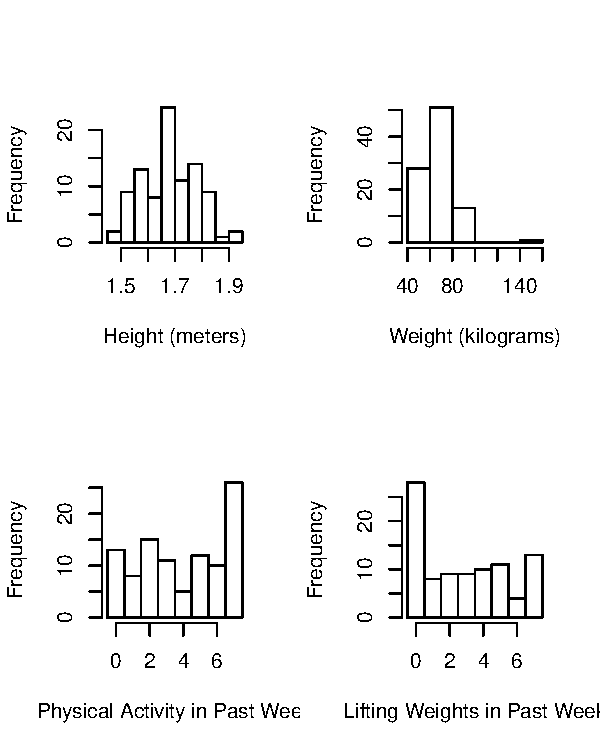
\includegraphics[width=\maxwidth]{figure/unnamed-chunk-72-1} 

}



\end{knitrout}

\section{Variability in Estimates}
The sample parameters can be calculated as well as the population parameters.  These correspond to the data seen in Table 4.5 in the main text.  
\begin{knitrout}
\definecolor{shadecolor}{rgb}{0.969, 0.969, 0.969}\color{fgcolor}\begin{kframe}
\begin{alltt}
\hlkwd{mean}\hlstd{(yrbss.sample}\hlopt{$}\hlstd{physically.active.7d,} \hlkwc{na.rm} \hlstd{=} \hlnum{TRUE}\hlstd{)}
\end{alltt}
\begin{verbatim}
## [1] 3.93
\end{verbatim}
\begin{alltt}
\hlkwd{mean}\hlstd{(yrbss}\hlopt{$}\hlstd{physically.active.7d,} \hlkwc{na.rm} \hlstd{=} \hlnum{TRUE}\hlstd{)}
\end{alltt}
\begin{verbatim}
## [1] 3.903005
\end{verbatim}
\begin{alltt}
\hlkwd{median}\hlstd{(yrbss.sample}\hlopt{$}\hlstd{physically.active.7d,} \hlkwc{na.rm} \hlstd{=} \hlnum{TRUE}\hlstd{)}
\end{alltt}
\begin{verbatim}
## [1] 4
\end{verbatim}
\begin{alltt}
\hlkwd{median}\hlstd{(yrbss}\hlopt{$}\hlstd{physically.active.7d,} \hlkwc{na.rm} \hlstd{=} \hlnum{TRUE}\hlstd{)}
\end{alltt}
\begin{verbatim}
## [1] 4
\end{verbatim}
\begin{alltt}
\hlkwd{sd}\hlstd{(yrbss.sample}\hlopt{$}\hlstd{physically.active.7d,} \hlkwc{na.rm} \hlstd{=} \hlnum{TRUE}\hlstd{)}
\end{alltt}
\begin{verbatim}
## [1] 2.535625
\end{verbatim}
\begin{alltt}
\hlkwd{sd}\hlstd{(yrbss}\hlopt{$}\hlstd{physically.active.7d,} \hlkwc{na.rm} \hlstd{=} \hlnum{TRUE}\hlstd{)}
\end{alltt}
\begin{verbatim}
## [1] 2.564105
\end{verbatim}
\end{kframe}
\end{knitrout}

\subsection{Sampling Distribution for the Mean}
The concept of a sampling distribution highlights the fact that sampling is a random process, and every sample is likely to be quite different than any other.  For this reason, sampling distributions are created, which represent the accumulated information of a large number of random samples.  

The following steps can be used to create a \textbf{sampling distribution of the sample mean}.  
\begin{knitrout}
\definecolor{shadecolor}{rgb}{0.969, 0.969, 0.969}\color{fgcolor}\begin{kframe}
\begin{alltt}
\hlcom{## Figure 4.7}
\hlcom{# Step 1: Create an empty list to put values in }
\hlstd{means} \hlkwb{=} \hlkwd{rep}\hlstd{(}\hlnum{NA}\hlstd{,} \hlnum{1000}\hlstd{)}

\hlcom{# Step 2: Use a "for" loop to collect 1000 samples }
\hlkwa{for}\hlstd{(ii} \hlkwa{in} \hlnum{1}\hlopt{:}\hlnum{1000}\hlstd{)\{}
  \hlcom{# Step 2a: Get the random sample }
  \hlstd{indeces} \hlkwb{=} \hlkwd{sample}\hlstd{(}\hlkwc{x} \hlstd{= (}\hlnum{1}\hlopt{:}\hlkwd{nrow}\hlstd{(yrbss)),} \hlkwc{size} \hlstd{=} \hlnum{100}\hlstd{,} \hlkwc{replace} \hlstd{=} \hlnum{FALSE}\hlstd{)}
  \hlstd{sample} \hlkwb{=} \hlstd{yrbss[indeces,]}
  \hlcom{# Step 2b: Take the mean of the sample and store it }
  \hlstd{means[ii]} \hlkwb{=} \hlkwd{mean}\hlstd{(sample}\hlopt{$}\hlstd{physically.active.7d,} \hlkwc{na.rm} \hlstd{=} \hlnum{TRUE}\hlstd{)}
\hlstd{\}}

\hlcom{# Step 3: Plot your results }
\hlkwd{par}\hlstd{(}\hlkwc{mfrow} \hlstd{=} \hlkwd{c}\hlstd{(}\hlnum{1}\hlstd{,}\hlnum{2}\hlstd{))}
\hlkwd{hist}\hlstd{(means,} \hlkwc{breaks} \hlstd{=} \hlnum{30}\hlstd{)}
\hlkwd{qqnorm}\hlstd{(means)}
\hlkwd{qqline}\hlstd{(means)}
\end{alltt}
\end{kframe}

{\centering 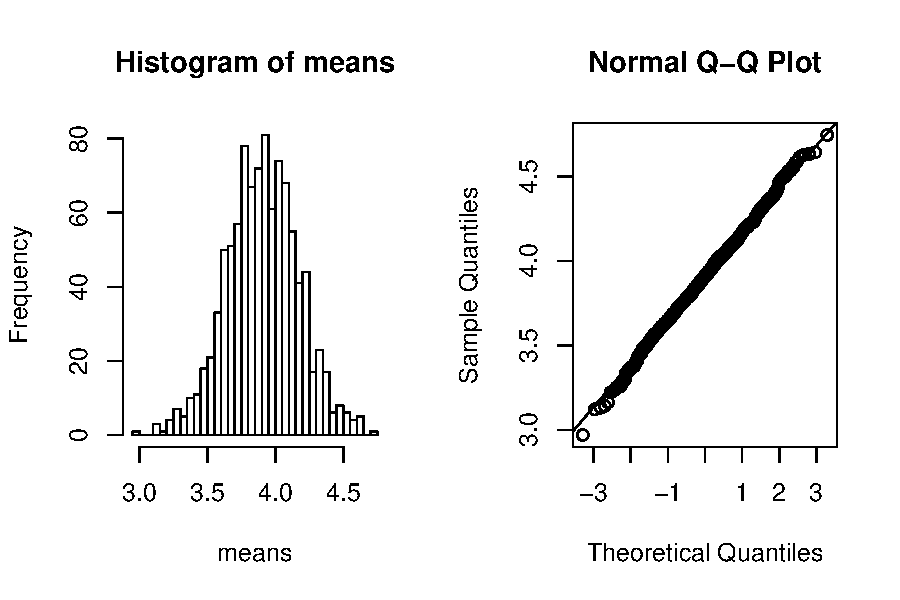
\includegraphics[width=\maxwidth]{figure/unnamed-chunk-74-1} 

}



\end{knitrout}
As discussed in chapter 3, the above plots are used to determine the normality of the sample.  The left plot is just a histogram, which can be inspected visually to see that it approximates a normal distribution.  The plot on the right is a more powerful tool for determining the normality - the dots represent deviation of data points from a theoretical normal distribution, as represented by the line on the plot.  The above plot shows a fairly normal distribution because of how closely the dots match the line.  

The more samples are taken, the more accurately will the distribution be depicted.  Figure 4.8 demonstrates this below 
\begin{knitrout}
\definecolor{shadecolor}{rgb}{0.969, 0.969, 0.969}\color{fgcolor}\begin{kframe}
\begin{alltt}
\hlcom{## Figure 4.8}
\hlstd{means} \hlkwb{=} \hlkwd{rep}\hlstd{(}\hlnum{NA}\hlstd{,} \hlnum{100000}\hlstd{)}
\hlkwa{for}\hlstd{(ii} \hlkwa{in} \hlnum{1}\hlopt{:}\hlnum{100000}\hlstd{)\{}
  \hlstd{indeces} \hlkwb{=} \hlkwd{sample}\hlstd{(}\hlkwc{x} \hlstd{= (}\hlnum{1}\hlopt{:}\hlkwd{nrow}\hlstd{(yrbss)),} \hlkwc{size} \hlstd{=} \hlnum{100}\hlstd{,} \hlkwc{replace} \hlstd{=} \hlnum{FALSE}\hlstd{)}
  \hlstd{sample} \hlkwb{=} \hlstd{yrbss[indeces,]}
  \hlstd{means[ii]} \hlkwb{=} \hlkwd{mean}\hlstd{(sample}\hlopt{$}\hlstd{physically.active.7d,} \hlkwc{na.rm} \hlstd{=} \hlnum{TRUE}\hlstd{)}
\hlstd{\}}

\hlkwd{par}\hlstd{(}\hlkwc{mfrow} \hlstd{=} \hlkwd{c}\hlstd{(}\hlnum{1}\hlstd{,}\hlnum{2}\hlstd{))}
\hlkwd{hist}\hlstd{(means,} \hlkwc{breaks} \hlstd{=} \hlnum{30}\hlstd{)}
\hlkwd{qqnorm}\hlstd{(means)}
\hlkwd{qqline}\hlstd{(means)}
\end{alltt}
\end{kframe}
\end{knitrout}

\section{Confidence Intervals}
The first formula introduced in the text for calculating confidence intervals is as follows, 
\[ \text{ point estimate } \pm 1.96 \cdot \text{SE } \] 
\begin{knitrout}
\definecolor{shadecolor}{rgb}{0.969, 0.969, 0.969}\color{fgcolor}\begin{kframe}
\begin{alltt}
\hlcom{## Example 4.3 }
\hlstd{xbar} \hlkwb{=} \hlkwd{mean}\hlstd{(yrbss.sample}\hlopt{$}\hlstd{physically.active.7d,} \hlkwc{na.rm} \hlstd{=} \hlnum{TRUE}\hlstd{)}
\hlstd{std.error} \hlkwb{=} \hlkwd{sd}\hlstd{(yrbss.sample}\hlopt{$}\hlstd{physically.active.7d,} \hlkwc{na.rm} \hlstd{=} \hlnum{TRUE}\hlstd{)}\hlopt{/}\hlkwd{sqrt}\hlstd{(}\hlkwd{length}\hlstd{(yrbss.sample}\hlopt{$}\hlstd{physically.active.7d))}
\hlstd{ci} \hlkwb{=} \hlkwd{c}\hlstd{(xbar} \hlopt{-} \hlnum{1.96}\hlopt{*}\hlstd{std.error, xbar} \hlopt{+} \hlnum{1.96}\hlopt{*}\hlstd{std.error)}
\hlstd{ci}
\end{alltt}
\begin{verbatim}
## [1] 3.433018 4.426982
\end{verbatim}
\end{kframe}
\end{knitrout}

To generalize this formula, a standard normal distribution can be used to obtain $z^*$, giving the following 
\[ \bar{x} \pm z^* \cdot \text{SE } \]
$R$ can be used to calculate $z^*$ and then using that value, to solve for the confidence interval.  A key point here is that we want the middle 95\% of the distribution, which divides the remaining 5\% between the two tails.  This is equivalent to 
\begin{knitrout}
\definecolor{shadecolor}{rgb}{0.969, 0.969, 0.969}\color{fgcolor}\begin{kframe}
\begin{alltt}
\hlcom{## Example 4.3 (version 2)}
\hlstd{perc} \hlkwb{=} \hlnum{.95}
\hlstd{z} \hlkwb{=} \hlkwd{qnorm}\hlstd{(}\hlkwc{p} \hlstd{= perc} \hlopt{+} \hlstd{(}\hlnum{1}\hlopt{-}\hlstd{perc)}\hlopt{/}\hlnum{2}\hlstd{,} \hlkwc{lower.tail} \hlstd{=} \hlnum{TRUE}\hlstd{)}
\hlstd{z}
\end{alltt}
\begin{verbatim}
## [1] 1.959964
\end{verbatim}
\begin{alltt}
\hlstd{ci} \hlkwb{=} \hlkwd{c}\hlstd{(xbar} \hlopt{-} \hlnum{1.96}\hlopt{*}\hlstd{std.error, xbar} \hlopt{+} \hlnum{1.96}\hlopt{*}\hlstd{std.error)}
\hlstd{ci}
\end{alltt}
\begin{verbatim}
## [1] 3.433018 4.426982
\end{verbatim}
\end{kframe}
\end{knitrout}

\begin{knitrout}
\definecolor{shadecolor}{rgb}{0.969, 0.969, 0.969}\color{fgcolor}\begin{kframe}
\begin{alltt}
\hlcom{## Example 4.6 }
\hlstd{perc} \hlkwb{=} \hlnum{.99}
\hlstd{z} \hlkwb{=} \hlkwd{qnorm}\hlstd{(}\hlkwc{p} \hlstd{= perc} \hlopt{+} \hlstd{(}\hlnum{1}\hlopt{-}\hlstd{perc)}\hlopt{/}\hlnum{2}\hlstd{,} \hlkwc{lower.tail} \hlstd{=} \hlnum{TRUE}\hlstd{)}
\hlstd{z}
\end{alltt}
\begin{verbatim}
## [1] 2.575829
\end{verbatim}
\end{kframe}
\end{knitrout}

\begin{knitrout}
\definecolor{shadecolor}{rgb}{0.969, 0.969, 0.969}\color{fgcolor}\begin{kframe}
\begin{alltt}
\hlcom{## Example 4.8 }
\hlstd{ci} \hlkwb{=} \hlkwd{c}\hlstd{(xbar} \hlopt{-} \hlstd{z}\hlopt{*}\hlstd{std.error, xbar} \hlopt{+} \hlstd{z}\hlopt{*}\hlstd{std.error)}
\hlstd{ci}
\end{alltt}
\begin{verbatim}
## [1] 3.276866 4.583134
\end{verbatim}
\end{kframe}
\end{knitrout}


Example 4.10 is an excellent example of how to clean up data.  The main text restricts the sample to adults over 21 with reported BMI values.  The steps below show how to find the individuals who are children or who have missing data and how to remove them from the sample.  Often times, when using a sample of a large population, a process similar to this one must be used.  Missing data can be problematic for analyses of the data, so understanding how to clean up the data appropriately is quite important. 
\begin{knitrout}
\definecolor{shadecolor}{rgb}{0.969, 0.969, 0.969}\color{fgcolor}\begin{kframe}
\begin{alltt}
\hlcom{## Example 4.10 }
\hlcom{# Collect the sample of size 200}
\hlkwd{set.seed}\hlstd{(}\hlnum{5011}\hlstd{)}
\hlstd{indeces} \hlkwb{=} \hlkwd{sample}\hlstd{(}\hlnum{1}\hlopt{:}\hlkwd{length}\hlstd{(NHANES}\hlopt{$}\hlstd{ID),} \hlkwc{size} \hlstd{=} \hlnum{200}\hlstd{)}
\hlstd{nhanes.sample} \hlkwb{=} \hlstd{NHANES[indeces,]}

\hlcom{# First remove the children from the sample}
\hlstd{children} \hlkwb{=} \hlkwd{which}\hlstd{(nhanes.sample}\hlopt{$}\hlstd{Age} \hlopt{<} \hlnum{21}\hlstd{)}  \hlcom{#Find children }
\hlstd{nhanes.sample} \hlkwb{=} \hlstd{nhanes.sample[}\hlopt{-}\hlstd{children, ]}       \hlcom{#Remove them from the sample}

\hlkwd{hist}\hlstd{(nhanes.sample}\hlopt{$}\hlstd{BMI,} \hlkwc{breaks} \hlstd{=} \hlstr{"FD"}\hlstd{)} \hlcom{## This gives Figure 4.10}
\end{alltt}
\end{kframe}

{\centering 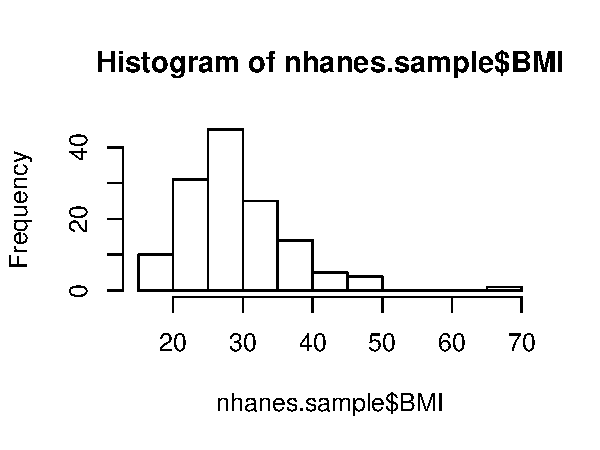
\includegraphics[width=\maxwidth]{figure/unnamed-chunk-80-1} 

}


\begin{kframe}\begin{alltt}
\hlcom{# Locate where the outlier is occuring }
\hlstd{x} \hlkwb{=} \hlkwd{which}\hlstd{(nhanes.sample}\hlopt{$}\hlstd{BMI} \hlopt{==} \hlkwd{max}\hlstd{(nhanes.sample}\hlopt{$}\hlstd{BMI,} \hlkwc{na.rm} \hlstd{=} \hlnum{TRUE}\hlstd{))}
\hlcom{# Remove the outlier }
\hlstd{nhanes.sample} \hlkwb{=} \hlstd{nhanes.sample[}\hlopt{-}\hlstd{x,]}
\hlcom{# Plot again to confirm that it was removed }
\hlkwd{hist}\hlstd{(nhanes.sample}\hlopt{$}\hlstd{BMI)}
\end{alltt}
\end{kframe}

{\centering 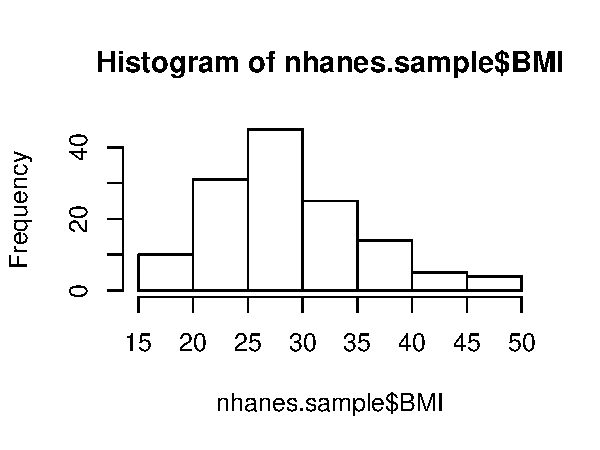
\includegraphics[width=\maxwidth]{figure/unnamed-chunk-80-2} 

}


\begin{kframe}\begin{alltt}
\hlcom{# Calculate sample statistics and confidence interval}
\hlstd{xbar} \hlkwb{=} \hlkwd{mean}\hlstd{(nhanes.sample}\hlopt{$}\hlstd{BMI,} \hlkwc{na.rm} \hlstd{=} \hlnum{TRUE}\hlstd{)}
\hlstd{n} \hlkwb{=} \hlkwd{length}\hlstd{(nhanes.sample}\hlopt{$}\hlstd{BMI)}
\hlstd{s} \hlkwb{=} \hlkwd{sd}\hlstd{(nhanes.sample}\hlopt{$}\hlstd{BMI,} \hlkwc{na.rm}\hlstd{=}\hlnum{TRUE}\hlstd{)}
\hlstd{se} \hlkwb{=} \hlstd{s}\hlopt{/}\hlkwd{sqrt}\hlstd{(n)}
\hlstd{perc} \hlkwb{=} \hlnum{.95}
\hlstd{z} \hlkwb{=} \hlkwd{qnorm}\hlstd{(}\hlkwc{p} \hlstd{= perc} \hlopt{+} \hlstd{(}\hlnum{1}\hlopt{-}\hlstd{perc)}\hlopt{/}\hlnum{2}\hlstd{,} \hlkwc{lower.tail} \hlstd{=} \hlnum{TRUE}\hlstd{)}
\hlstd{ci} \hlkwb{=} \hlkwd{c}\hlstd{(xbar} \hlopt{-} \hlstd{z}\hlopt{*}\hlstd{se, xbar} \hlopt{+} \hlstd{z}\hlopt{*}\hlstd{se)}
\hlstd{ci}
\end{alltt}
\begin{verbatim}
## [1] 27.66076 29.94282
\end{verbatim}
\end{kframe}
\end{knitrout}

\section{Hypothesis Testing}
If you have calculated your test statistic by hand, $R$ can easily be used to get the p-value using the function \textit{pnorm()} as in Chapter 3.  The example that is worked through in the main text can be completed as follows.  Note that \textit{lower.tail = FALSE} because the alternative hypothesis here is 
\[ H_A: \mu_{bmi} > 21.7 \]
which implies that the upper tail must be considered.  
\begin{knitrout}
\definecolor{shadecolor}{rgb}{0.969, 0.969, 0.969}\color{fgcolor}\begin{kframe}
\begin{alltt}
\hlstd{mu} \hlkwb{=} \hlnum{21.7}
\hlstd{t} \hlkwb{=} \hlstd{(xbar} \hlopt{-} \hlstd{mu)}\hlopt{/}\hlstd{(s}\hlopt{/}\hlkwd{sqrt}\hlstd{(n))}
\hlstd{t}
\end{alltt}
\begin{verbatim}
## [1] 12.19889
\end{verbatim}
\begin{alltt}
\hlkwd{pnorm}\hlstd{(t,} \hlkwc{lower.tail} \hlstd{=} \hlnum{FALSE}\hlstd{)}
\end{alltt}
\begin{verbatim}
## [1] 1.575536e-34
\end{verbatim}
\end{kframe}
\end{knitrout}

In $R$, all of the steps of hypothesis testing can be done with one single function, \textit{t.test()}.  This gives the test statistic, the p-value, and the confidence interval.  The function takes the data as an argument, $x$, the null hypothesis value, as $mu$, and the alternative hypothesis type, as $alternative$, which can be \textit{"less", "greater",} or \textit{"two.sided"}.  

The example shown below gives a comparison of doing the method by hand, as well as using the function.  
\begin{knitrout}
\definecolor{shadecolor}{rgb}{0.969, 0.969, 0.969}\color{fgcolor}\begin{kframe}
\begin{alltt}
\hlcom{## Example 4.13}
\hlkwd{set.seed}\hlstd{(}\hlnum{5011}\hlstd{)}
\hlstd{indeces} \hlkwb{=} \hlkwd{sample}\hlstd{(}\hlnum{1}\hlopt{:}\hlkwd{length}\hlstd{(NHANES}\hlopt{$}\hlstd{ID),} \hlkwc{size} \hlstd{=} \hlnum{200}\hlstd{)}
\hlstd{nhanes.sample} \hlkwb{=} \hlstd{NHANES[indeces,]}

\hlcom{# First remove the children from the sample}
\hlstd{children} \hlkwb{=} \hlkwd{which}\hlstd{(nhanes.sample}\hlopt{$}\hlstd{Age} \hlopt{<} \hlnum{21}\hlstd{)}  \hlcom{#Find children }
\hlstd{nhanes.sample} \hlkwb{=} \hlstd{nhanes.sample[}\hlopt{-}\hlstd{children, ]}

\hlcom{# Method 1 }
\hlstd{xbar} \hlkwb{=} \hlkwd{mean}\hlstd{(nhanes.sample}\hlopt{$}\hlstd{SleepHrsNight,} \hlkwc{na.rm} \hlstd{=} \hlnum{TRUE}\hlstd{)}
\hlstd{s} \hlkwb{=} \hlkwd{sd}\hlstd{(nhanes.sample}\hlopt{$}\hlstd{SleepHrsNight,} \hlkwc{na.rm} \hlstd{=} \hlnum{TRUE}\hlstd{)}
\hlstd{mu} \hlkwb{=} \hlnum{7}
\hlstd{n} \hlkwb{=} \hlkwd{length}\hlstd{(nhanes.sample}\hlopt{$}\hlstd{SleepHrsNight)}
\hlstd{t} \hlkwb{=} \hlstd{(xbar} \hlopt{-} \hlstd{mu)}\hlopt{/}\hlstd{(s}\hlopt{/}\hlkwd{sqrt}\hlstd{(n))}
\hlstd{t}
\end{alltt}
\begin{verbatim}
## [1] -0.864111
\end{verbatim}
\begin{alltt}
\hlstd{p} \hlkwb{=} \hlkwd{pnorm}\hlstd{(t,} \hlkwc{lower.tail} \hlstd{=} \hlnum{TRUE}\hlstd{)}
\hlstd{p}
\end{alltt}
\begin{verbatim}
## [1] 0.1937634
\end{verbatim}
\begin{alltt}
\hlcom{# Method 2 }
\hlkwd{t.test}\hlstd{(}\hlkwc{x} \hlstd{= nhanes.sample}\hlopt{$}\hlstd{SleepHrsNight,} \hlkwc{mu} \hlstd{= mu,} \hlkwc{alternative} \hlstd{=} \hlstr{"less"}\hlstd{)}
\end{alltt}
\begin{verbatim}
## 
## 	One Sample t-test
## 
## data:  nhanes.sample$SleepHrsNight
## t = -0.8641, df = 134, p-value = 0.1945
## alternative hypothesis: true mean is less than 7
## 95 percent confidence interval:
##      -Inf 7.095073
## sample estimates:
## mean of x 
##  6.896296
\end{verbatim}
\end{kframe}
\end{knitrout}


\newpage
\chapter{Inference For Numerical Data}
\minitoc

\vspace{0.5cm} 

\section{The t-distribution}
The main text introduces the \textbf{t-distribution} and explains under what circumstances it should be used.  Using it in in R is very similar to many concepts seen through Chapter 4 thus far.  

The following plot shows how the t-distribution approximates the normal distribution as the degrees of freedom grow.  The use of the function \textit{dt()} parallels the use of \textit{dnorm()} as has been used in previous chapters.  

\begin{knitrout}
\definecolor{shadecolor}{rgb}{0.969, 0.969, 0.969}\color{fgcolor}\begin{kframe}
\begin{alltt}
\hlcom{## Figure 5.2 getting the x-axis values}
\hlstd{x} \hlkwb{=} \hlkwd{seq}\hlstd{(}\hlopt{-}\hlnum{5}\hlstd{,} \hlnum{9}\hlstd{,} \hlnum{0.1}\hlstd{)}

\hlcom{# finding the corresponding distribution values for several distributions}
\hlstd{t1} \hlkwb{=} \hlkwd{dt}\hlstd{(x,} \hlkwc{df} \hlstd{=} \hlnum{1}\hlstd{)}
\hlstd{t2} \hlkwb{=} \hlkwd{dt}\hlstd{(x,} \hlkwc{df} \hlstd{=} \hlnum{2}\hlstd{)}
\hlstd{t4} \hlkwb{=} \hlkwd{dt}\hlstd{(x,} \hlkwc{df} \hlstd{=} \hlnum{4}\hlstd{)}
\hlstd{t8} \hlkwb{=} \hlkwd{dt}\hlstd{(x,} \hlkwc{df} \hlstd{=} \hlnum{8}\hlstd{)}
\hlstd{norm} \hlkwb{=} \hlkwd{dnorm}\hlstd{(x)}

\hlcom{# plotting the results, with custom colors}
\hlkwd{plot}\hlstd{(x, t1,} \hlkwc{type} \hlstd{=} \hlstr{"l"}\hlstd{,} \hlkwc{ylim} \hlstd{=} \hlkwd{c}\hlstd{(}\hlnum{0}\hlstd{,} \hlnum{0.4}\hlstd{),} \hlkwc{xlab} \hlstd{=} \hlstr{""}\hlstd{,} \hlkwc{ylab} \hlstd{=} \hlstr{""}\hlstd{,} \hlkwc{col} \hlstd{=} \hlkwd{rgb}\hlstd{(}\hlnum{0}\hlstd{,}
    \hlnum{0}\hlstd{,} \hlnum{1}\hlstd{,} \hlkwc{alpha} \hlstd{=} \hlnum{0.1}\hlstd{))}
\hlkwd{lines}\hlstd{(x, t2,} \hlkwc{col} \hlstd{=} \hlkwd{rgb}\hlstd{(}\hlnum{0}\hlstd{,} \hlnum{0}\hlstd{,} \hlnum{1}\hlstd{,} \hlkwc{alpha} \hlstd{=} \hlnum{0.2}\hlstd{))}
\hlkwd{lines}\hlstd{(x, t4,} \hlkwc{col} \hlstd{=} \hlkwd{rgb}\hlstd{(}\hlnum{0}\hlstd{,} \hlnum{0}\hlstd{,} \hlnum{1}\hlstd{,} \hlkwc{alpha} \hlstd{=} \hlnum{0.3}\hlstd{))}
\hlkwd{lines}\hlstd{(x, t8,} \hlkwc{col} \hlstd{=} \hlkwd{rgb}\hlstd{(}\hlnum{0}\hlstd{,} \hlnum{0}\hlstd{,} \hlnum{1}\hlstd{,} \hlkwc{alpha} \hlstd{=} \hlnum{0.4}\hlstd{))}
\hlkwd{lines}\hlstd{(x, norm,} \hlkwc{col} \hlstd{=} \hlkwd{rgb}\hlstd{(}\hlnum{0}\hlstd{,} \hlnum{0}\hlstd{,} \hlnum{1}\hlstd{,} \hlkwc{alpha} \hlstd{=} \hlnum{0.5}\hlstd{))}
\end{alltt}
\end{kframe}

{\centering 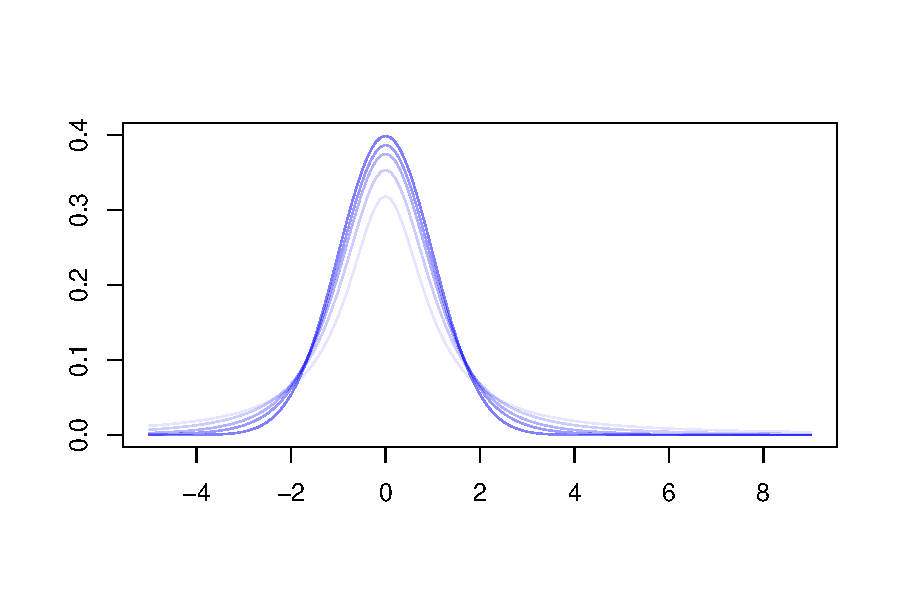
\includegraphics[width=\maxwidth]{figure/unnamed-chunk-83-1} 

}



\end{knitrout}

\subsection{The Alternative to t-Tables}
The main text talks through the use of a \textbf{t-table}, but this text will go through examples of using software to do the same calculations.  In $R$, the command of interests here are \textit{pt()} to get the percentage of the distribution above or below a certain value and \textit{qt()} to get distribution values for which a certain percentage of the distribution falls above.  The command \textit{pt()} takes values inside the t-table to return the values on the x-axis of the table, whereas \textit{qt()} returns values within the table when given values along the upper x-axis.  

An example of a one-sided calculation using the t-distribution can be viewed in Example 5.1 below.  Note the use of the stipulation \textit{lower.tail = TRUE} which ensures that the calculation is of values in the lower tail, i.e. those values which are less than -2.1.  
\begin{knitrout}
\definecolor{shadecolor}{rgb}{0.969, 0.969, 0.969}\color{fgcolor}\begin{kframe}
\begin{alltt}
\hlcom{## Example 5.1 }
\hlkwd{pt}\hlstd{(}\hlopt{-}\hlnum{2.1}\hlstd{,} \hlkwc{df} \hlstd{=} \hlnum{18}\hlstd{,} \hlkwc{lower.tail} \hlstd{=} \hlnum{TRUE}\hlstd{)}
\end{alltt}
\begin{verbatim}
## [1] 0.0250452
\end{verbatim}
\end{kframe}
\end{knitrout}

Example 5.2 shows a two sided calculation using the t-distribution.  In order to do this in $R$, each tail can be calculated separately and then the two values summed.  Alternatively, the symmetry of the t-distribution can be utilized to calculate one tail and multiply it by two.  
\begin{knitrout}
\definecolor{shadecolor}{rgb}{0.969, 0.969, 0.969}\color{fgcolor}\begin{kframe}
\begin{alltt}
\hlcom{## Example 5.2 }
\hlcom{# Method 1: calculate each tail and sum }
\hlkwd{pt}\hlstd{(}\hlnum{1.65}\hlstd{,} \hlkwc{df} \hlstd{=} \hlnum{20}\hlstd{,} \hlkwc{lower.tail} \hlstd{=} \hlnum{FALSE}\hlstd{)} \hlopt{+} \hlkwd{pt}\hlstd{(}\hlopt{-}\hlnum{1.65}\hlstd{,} \hlkwc{df} \hlstd{=} \hlnum{20}\hlstd{,} \hlkwc{lower.tail} \hlstd{=} \hlnum{TRUE}\hlstd{)}
\end{alltt}
\begin{verbatim}
## [1] 0.1145608
\end{verbatim}
\begin{alltt}
\hlcom{# Method 2: calculate one tail and multiply by 2 }
\hlnum{2}\hlopt{*}\hlkwd{pt}\hlstd{(}\hlnum{1.65}\hlstd{,} \hlkwc{df} \hlstd{=} \hlnum{20}\hlstd{,} \hlkwc{lower.tail} \hlstd{=} \hlnum{FALSE}\hlstd{)}
\end{alltt}
\begin{verbatim}
## [1] 0.1145608
\end{verbatim}
\end{kframe}
\end{knitrout}


\subsection{Confidence Intervals}
As in chapter 4, confidence intervals using the t-distribution can be set up in the same way with a $t^*$ value instead of a $z^*$ value.  

\begin{knitrout}
\definecolor{shadecolor}{rgb}{0.969, 0.969, 0.969}\color{fgcolor}\begin{kframe}
\begin{alltt}
\hlcom{## Example 5.3 }
\hlstd{n} \hlkwb{=} \hlnum{19}
\hlstd{xbar} \hlkwb{=} \hlnum{4.4}
\hlstd{s} \hlkwb{=} \hlnum{2.3}
\hlstd{std.error} \hlkwb{=} \hlstd{s}\hlopt{/}\hlkwd{sqrt}\hlstd{(n)}
\hlstd{perc} \hlkwb{=} \hlnum{.95}
\hlstd{t.star} \hlkwb{=} \hlkwd{qt}\hlstd{(}\hlkwc{p} \hlstd{= perc} \hlopt{+} \hlstd{(}\hlnum{1}\hlopt{-}\hlstd{perc)}\hlopt{/}\hlnum{2}\hlstd{,} \hlkwc{df} \hlstd{= n}\hlopt{-}\hlnum{1}\hlstd{,} \hlkwc{lower.tail} \hlstd{=} \hlnum{TRUE}\hlstd{)}
\hlstd{ci} \hlkwb{=} \hlkwd{c}\hlstd{(xbar} \hlopt{-} \hlstd{t.star}\hlopt{*}\hlstd{std.error, xbar} \hlopt{+} \hlstd{t.star}\hlopt{*}\hlstd{std.error)}
\hlstd{ci}
\end{alltt}
\begin{verbatim}
## [1] 3.291435 5.508565
\end{verbatim}
\end{kframe}
\end{knitrout}

\begin{knitrout}
\definecolor{shadecolor}{rgb}{0.969, 0.969, 0.969}\color{fgcolor}\begin{kframe}
\begin{alltt}
\hlcom{## Example 5.5 }
\hlstd{mu} \hlkwb{=} \hlnum{0.5}
\hlstd{n} \hlkwb{=} \hlnum{15}
\hlstd{xbar} \hlkwb{=} \hlnum{0.287}
\hlstd{s} \hlkwb{=} \hlnum{0.069}
\hlstd{std.error} \hlkwb{=} \hlstd{s}\hlopt{/}\hlkwd{sqrt}\hlstd{(n)}
\hlstd{t} \hlkwb{=} \hlstd{(xbar} \hlopt{-} \hlstd{mu)}\hlopt{/}\hlstd{std.error}
\hlkwd{pt}\hlstd{(t,} \hlkwc{df} \hlstd{= n}\hlopt{-}\hlnum{1}\hlstd{)}
\end{alltt}
\begin{verbatim}
## [1] 4.903809e-09
\end{verbatim}
\end{kframe}
\end{knitrout}

\section{Paired Data} 
When working with paired data, several methods can be used to measure the effect.  The first method is to calculate by hand differences between the pairs and then to perform a standard t-test as follows.  
\begin{knitrout}
\definecolor{shadecolor}{rgb}{0.969, 0.969, 0.969}\color{fgcolor}\begin{kframe}
\begin{alltt}
\hlcom{## Example 5.6 }
\hlstd{diff} \hlkwb{=} \hlstd{swim}\hlopt{$}\hlstd{wet.suit.velocity} \hlopt{-} \hlstd{swim}\hlopt{$}\hlstd{swim.suit.velocity}
\hlkwd{t.test}\hlstd{(diff,} \hlkwc{mu} \hlstd{=} \hlnum{0}\hlstd{,} \hlkwc{alternative} \hlstd{=} \hlstr{"two.sided"}\hlstd{)}
\end{alltt}
\begin{verbatim}
## 
## 	One Sample t-test
## 
## data:  diff
## t = 3.7019, df = 11, p-value = 0.00349
## alternative hypothesis: true mean is not equal to 0
## 95 percent confidence interval:
##  0.02534062 0.09965938
## sample estimates:
## mean of x 
##    0.0625
\end{verbatim}
\end{kframe}
\end{knitrout}

The second method involves using a \textbf{paired t-test}, which performs the same operation without the direct calculation of the differences being required first.  It can be seen that the output of this test is the exact same as the test above.  This is a nice example of $R$ taking out a lot of the computational work.  
\begin{knitrout}
\definecolor{shadecolor}{rgb}{0.969, 0.969, 0.969}\color{fgcolor}\begin{kframe}
\begin{alltt}
\hlkwd{t.test}\hlstd{(swim}\hlopt{$}\hlstd{wet.suit.velocity, swim}\hlopt{$}\hlstd{swim.suit.velocity,} \hlkwc{paired} \hlstd{=} \hlnum{TRUE}\hlstd{)}
\end{alltt}
\begin{verbatim}
## 
## 	Paired t-test
## 
## data:  swim$wet.suit.velocity and swim$swim.suit.velocity
## t = 3.7019, df = 11, p-value = 0.00349
## alternative hypothesis: true difference in means is not equal to 0
## 95 percent confidence interval:
##  0.02534062 0.09965938
## sample estimates:
## mean of the differences 
##                  0.0625
\end{verbatim}
\end{kframe}
\end{knitrout}

\section{Difference of Two Means} 
%% COME BACK HERE 


\subsection{Hypothesis Tests for a Different in Means}
In order to perform a \textbf{two-sample t-test}, there are again two methods.  The first involves dividing the data into two samples (unless the data has already come separated) and performing a t-test.  The second has $R$ do the entire process.  Note that for this method, the tilde signifies the grouping variable.  So in this case, the \textit{weight} data is grouped by the variable \textit{smoke}.  
\begin{knitrout}
\definecolor{shadecolor}{rgb}{0.969, 0.969, 0.969}\color{fgcolor}\begin{kframe}
\begin{alltt}
\hlcom{## Example 5.11 }
\hlcom{# Method 1: divide the data by hand }
\hlstd{smoker} \hlkwb{=} \hlstd{baby.smoke}\hlopt{$}\hlstd{weight[baby.smoke}\hlopt{$}\hlstd{smoke} \hlopt{==} \hlstr{"smoker"}\hlstd{]}
\hlstd{non.smoker} \hlkwb{=} \hlstd{baby.smoke}\hlopt{$}\hlstd{weight[baby.smoke}\hlopt{$}\hlstd{smoke} \hlopt{==} \hlstr{"nonsmoker"}\hlstd{]}
\hlkwd{t.test}\hlstd{(non.smoker, smoker)}
\end{alltt}
\begin{verbatim}
## 
## 	Welch Two Sample t-test
## 
## data:  non.smoker and smoker
## t = 1.4967, df = 89.277, p-value = 0.138
## alternative hypothesis: true difference in means is not equal to 0
## 95 percent confidence interval:
##  -0.1311663  0.9321663
## sample estimates:
## mean of x mean of y 
##    7.1795    6.7790
\end{verbatim}
\begin{alltt}
\hlcom{# Method 2: R does it all }
\hlkwd{t.test}\hlstd{(baby.smoke}\hlopt{$}\hlstd{weight}\hlopt{~}\hlstd{baby.smoke}\hlopt{$}\hlstd{smoke)}
\end{alltt}
\begin{verbatim}
## 
## 	Welch Two Sample t-test
## 
## data:  baby.smoke$weight by baby.smoke$smoke
## t = 1.4967, df = 89.277, p-value = 0.138
## alternative hypothesis: true difference in means is not equal to 0
## 95 percent confidence interval:
##  -0.1311663  0.9321663
## sample estimates:
## mean in group nonsmoker    mean in group smoker 
##                  7.1795                  6.7790
\end{verbatim}
\end{kframe}
\end{knitrout}

\subsection{Pooled t-test} 
Performing what is known as a \textbf{pooled t-test} is very simple in $R$.  The procedure is the same as a two-sample t-test, with the addition of the clause \textit{var.equal = TRUE} in the \textit{t.test()} command.  This is because a pooled t-test relies on the assumption of nearly equal variance between the two samples.  For example, performing the same test as above but using a pooled t-test would look like the following, 
\begin{knitrout}
\definecolor{shadecolor}{rgb}{0.969, 0.969, 0.969}\color{fgcolor}\begin{kframe}
\begin{alltt}
\hlkwd{t.test}\hlstd{(baby.smoke}\hlopt{$}\hlstd{weight}\hlopt{~}\hlstd{baby.smoke}\hlopt{$}\hlstd{smoke,} \hlkwc{var.equal} \hlstd{=} \hlnum{TRUE}\hlstd{)}
\end{alltt}
\begin{verbatim}
## 
## 	Two Sample t-test
## 
## data:  baby.smoke$weight by baby.smoke$smoke
## t = 1.5517, df = 148, p-value = 0.1229
## alternative hypothesis: true difference in means is not equal to 0
## 95 percent confidence interval:
##  -0.1095531  0.9105531
## sample estimates:
## mean in group nonsmoker    mean in group smoker 
##                  7.1795                  6.7790
\end{verbatim}
\end{kframe}
\end{knitrout}


%% WHAT SHOULD I DO ABOUT ALL OF THE POWER STUFF??? NOT REALLY SURE R IS APPROPRIATE FOR A LOT OF THIS 

\stepcounter{section}
\section{ANOVA} 
The main text walks through the arithmetic procedures of the ANOVA test and calculating the F-statistic.  $R$ makes this process much simpler, such that the entire calculation can be performed with just one line of code.  The command \textit{anova()} takes as its input a linear regression model.  Chapter 6 will go into much more detail about linear regression, but for now, note that within the function \textit{lm()}, the first variable before the tilde is the one for which the means are being compared, while the second variable after the tilde specifies the groups.  The command below works out Example 5.22 from the main text, getting the same $F$ statistic as the hand calculated value.  

\begin{knitrout}
\definecolor{shadecolor}{rgb}{0.969, 0.969, 0.969}\color{fgcolor}\begin{kframe}
\begin{alltt}
\hlcom{## Example 5.22 }
\hlkwd{anova}\hlstd{(}\hlkwd{lm}\hlstd{(famuss}\hlopt{$}\hlstd{ndrm.ch} \hlopt{~} \hlstd{famuss}\hlopt{$}\hlstd{actn3.r577x))}
\end{alltt}
\begin{verbatim}
## Analysis of Variance Table
## 
## Response: famuss$ndrm.ch
##                     Df Sum Sq Mean Sq F value  Pr(>F)  
## famuss$actn3.r577x   2   7043  3521.6  3.2308 0.04022 *
## Residuals          592 645293  1090.0                  
## ---
## Signif. codes:  0 '***' 0.001 '**' 0.01 '*' 0.05 '.' 0.1 ' ' 1
\end{verbatim}
\end{kframe}
\end{knitrout}

\newpage
\chapter{Simple Linear Regression}
\minitoc

\vspace{0.5cm} 

\section{Checking Assumptions}
Before going into a discussion of linear regression itself, an investigation into the appropriateness of its use must first be conducted.  The main text walks through the four assumptions necessary to use an approximation to linearity, which are as follows 
\begin{enumerate}
\item Linearity 
\item Constant Variability 
\item Independent Observations
\item Residuals that are approximately normally distributed 
\end{enumerate}

There are various methods to check each of these assumptions, which should be investigated before the use of linear regression.  This next section goes through these methods and several examples.  

\subsection{Linearity}
To check for linearity, a simple examination of a scatterplot of the data will suffice.  The goal is to look for data such that a straight line can be drawn which appropriately represents the data.   The plot of Figure 6.1 below shows that $age$ and $RFFT$ appear to have a linear relationship. The inclusion of the command \textit{cex = 0.4} simply changes the size of the dots on the scatterplot, making them 40\% of their original size.  

\begin{knitrout}
\definecolor{shadecolor}{rgb}{0.969, 0.969, 0.969}\color{fgcolor}\begin{kframe}
\begin{alltt}
\hlcom{## Figure 6.1 First collecting the data sample}
\hlkwd{set.seed}\hlstd{(}\hlnum{5011}\hlstd{)}
\hlstd{row.num} \hlkwb{=} \hlkwd{sample}\hlstd{(}\hlnum{1}\hlopt{:}\hlkwd{nrow}\hlstd{(statins),} \hlnum{500}\hlstd{,} \hlkwc{replace} \hlstd{=} \hlnum{FALSE}\hlstd{)}
\hlstd{statins.samp} \hlkwb{=} \hlstd{statins[row.num, ]}

\hlcom{# Then plotting it}
\hlkwd{plot}\hlstd{(statins.samp}\hlopt{$}\hlstd{RFFT} \hlopt{~} \hlstd{statins.samp}\hlopt{$}\hlstd{Age,} \hlkwc{cex} \hlstd{=} \hlnum{0.4}\hlstd{,} \hlkwc{ylab} \hlstd{=} \hlstr{"RFFT Score"}\hlstd{,} \hlkwc{xlab} \hlstd{=} \hlstr{"Age (yrs)"}\hlstd{,}
    \hlkwc{main} \hlstd{=} \hlstr{""}\hlstd{)}
\end{alltt}
\end{kframe}

{\centering 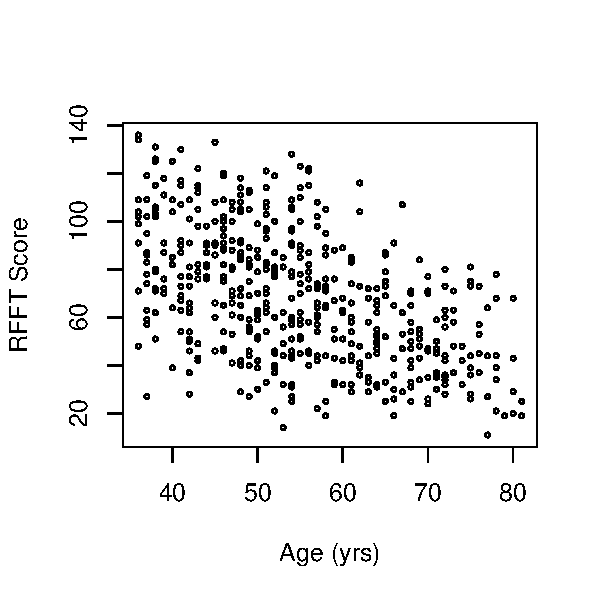
\includegraphics[width=\maxwidth]{figure/unnamed-chunk-93-1} 

}



\end{knitrout}

As further examples, the figures below show other linear relatonships.  
\begin{knitrout}
\definecolor{shadecolor}{rgb}{0.969, 0.969, 0.969}\color{fgcolor}\begin{kframe}
\begin{alltt}
\hlkwd{par}\hlstd{(}\hlkwc{mfrow} \hlstd{=} \hlkwd{c}\hlstd{(}\hlnum{1}\hlstd{,} \hlnum{2}\hlstd{))}
\hlcom{## Figure 6.2}
\hlkwd{plot}\hlstd{(frog.altitude.data}\hlopt{$}\hlstd{clutch.volume} \hlopt{~} \hlstd{frog.altitude.data}\hlopt{$}\hlstd{body.size,} \hlkwc{ylab} \hlstd{=} \hlstr{"Clutch Volume (mm3)"}\hlstd{,}
    \hlkwc{xlab} \hlstd{=} \hlstr{"Female Body Size (cm)"}\hlstd{)}

\hlkwd{plot}\hlstd{(famuss}\hlopt{$}\hlstd{weight, famuss}\hlopt{$}\hlstd{bmi)}
\end{alltt}
\end{kframe}

{\centering 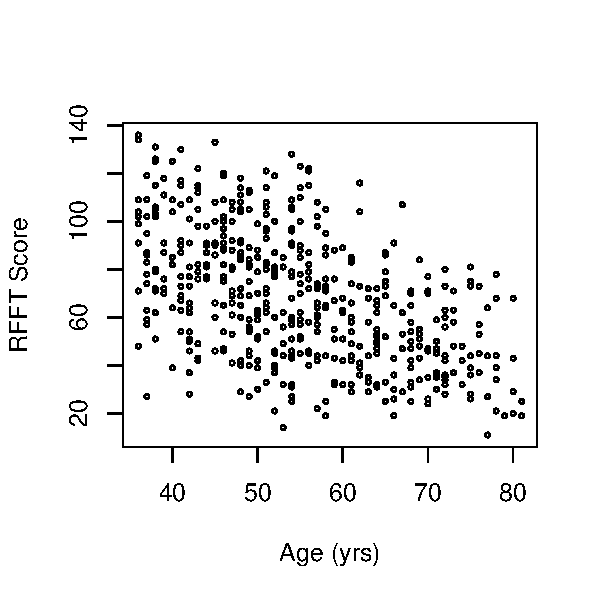
\includegraphics[width=\maxwidth]{figure/unnamed-chunk-94-1} 

}



\end{knitrout}

For comparison, the following plot shows data that a linear relationship is not appropriate for.  The first example shows data that appears to have no relationship, as indicated by the lack of trend in the scatterplot.  The second example shows a pattern that would be difficult to capture with a single straight line.  

\begin{knitrout}
\definecolor{shadecolor}{rgb}{0.969, 0.969, 0.969}\color{fgcolor}\begin{kframe}
\begin{alltt}
\hlkwd{par}\hlstd{(}\hlkwc{mfrow} \hlstd{=} \hlkwd{c}\hlstd{(}\hlnum{1}\hlstd{,} \hlnum{2}\hlstd{))}
\hlkwd{plot}\hlstd{(famuss}\hlopt{$}\hlstd{height, famuss}\hlopt{$}\hlstd{age)}
\hlkwd{plot}\hlstd{(frog.altitude.data}\hlopt{$}\hlstd{body.size, frog.altitude.data}\hlopt{$}\hlstd{egg.size)}
\end{alltt}
\end{kframe}

{\centering 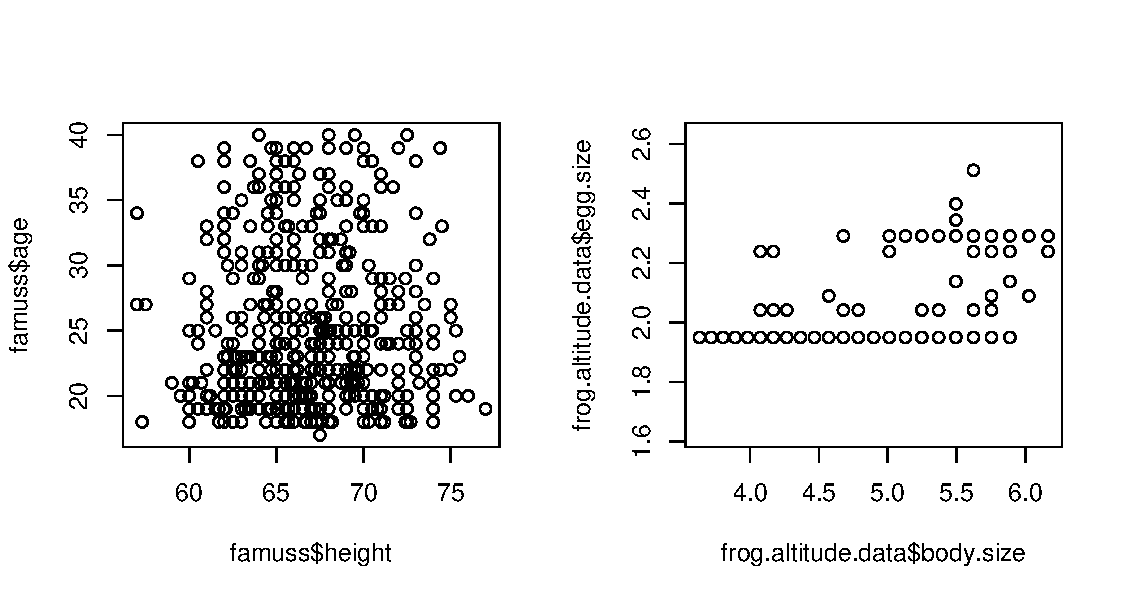
\includegraphics[width=\maxwidth]{figure/unnamed-chunk-95-1} 

}



\end{knitrout}

\subsection{Constant Variability}
To check for \textbf{constant variability}, a scatterplot is again a good resource.  Both Figure 6.1 and Figure 6.2 above show strong examples of constant variability.  For comparison, a few examples of non-constant variability are included here.  Notice how in the plot on the left, there is less variability in the clutch volumes with small egg size in comparison to the values with higher egg size.  Similarly, there is more variability in change in arm strength for lower weight individuals than for higher weight individuals.  


\begin{knitrout}
\definecolor{shadecolor}{rgb}{0.969, 0.969, 0.969}\color{fgcolor}\begin{kframe}
\begin{alltt}
\hlkwd{par}\hlstd{(}\hlkwc{mfrow} \hlstd{=} \hlkwd{c}\hlstd{(}\hlnum{1}\hlstd{,} \hlnum{2}\hlstd{))}
\hlkwd{plot}\hlstd{(frog.altitude.data}\hlopt{$}\hlstd{clutch.volume} \hlopt{~} \hlstd{frog.altitude.data}\hlopt{$}\hlstd{egg.size,} \hlkwc{main} \hlstd{=} \hlstr{"Variance Increasing with Egg Size"}\hlstd{,}
    \hlkwc{xlab} \hlstd{=} \hlstr{"Egg Size"}\hlstd{,} \hlkwc{ylab} \hlstd{=} \hlstr{"Clutch Volume"}\hlstd{)}
\hlkwd{plot}\hlstd{(famuss}\hlopt{$}\hlstd{ndrm.ch} \hlopt{~} \hlstd{famuss}\hlopt{$}\hlstd{weight,} \hlkwc{main} \hlstd{=} \hlstr{"Variance Decreasing with Weight"}\hlstd{,}
    \hlkwc{xlab} \hlstd{=} \hlstr{"Weight"}\hlstd{,} \hlkwc{ylab} \hlstd{=} \hlstr{"Change in Arm Strength"}\hlstd{)}
\end{alltt}
\end{kframe}

{\centering 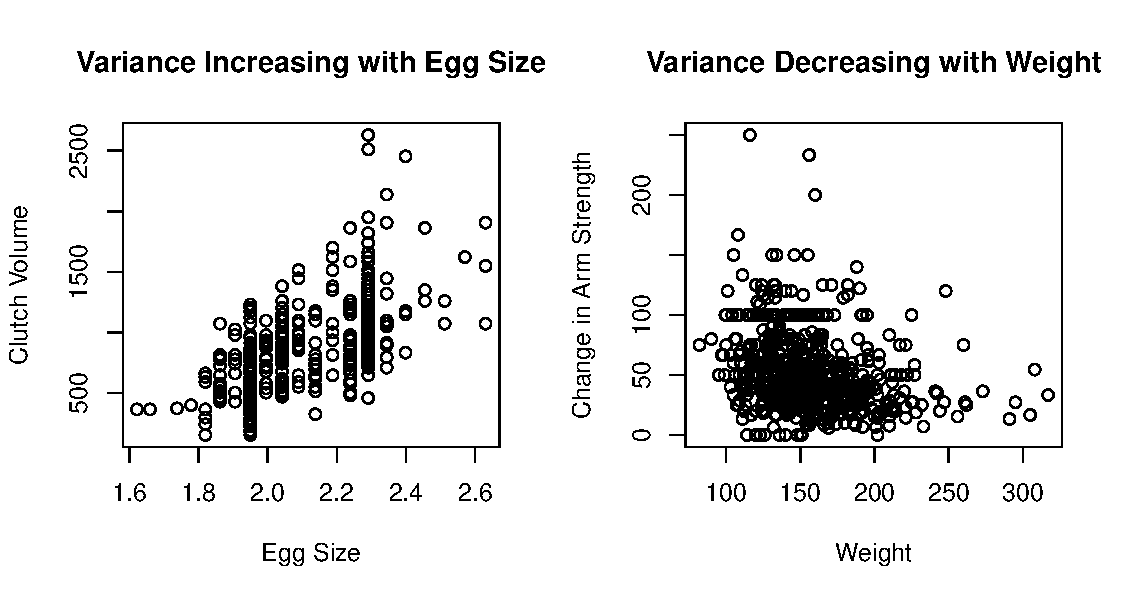
\includegraphics[width=\maxwidth]{figure/unnamed-chunk-96-1} 

}



\end{knitrout}

\subsection{Independence of Observations}
The assumption of \textbf{independence of observations} is less easily understood through physical study of the data.  Instead, the nature of the data and its parameters must be understood.  For example, some questions to consider include 
\begin{itemize}
\item Do the data points depend on each other? 
\item Is there a known relationship between some or all data points? 
\item Are the data points from the same individual, region, or time? 
\end{itemize}

\subsection{Normally Distributed Residuals}
In $R$, a plot of the residuals can be visualized to determine if this assumption is met.  First, to obtain the residuals, the linear regression must be obtained, using the command \textit{lm()}.  Then, the residuals of this model can be calculated using the command \textit{resid()} on the linear regression.  


These residuals can be visualized in a few ways: as a histogram, as a plot, or using \textit{qnorm()} and \textit{qqline()}.


Two examples of this procedure are included below.  In the first example, the residuals appear very close to normal.  This is a strong sign that the assumption is met.  

\begin{knitrout}
\definecolor{shadecolor}{rgb}{0.969, 0.969, 0.969}\color{fgcolor}\begin{kframe}
\begin{alltt}
\hlkwd{par}\hlstd{(}\hlkwc{mfrow} \hlstd{=} \hlkwd{c}\hlstd{(}\hlnum{1}\hlstd{,} \hlnum{3}\hlstd{))}
\hlstd{residuals} \hlkwb{=} \hlkwd{resid}\hlstd{(}\hlkwd{lm}\hlstd{(statins.samp}\hlopt{$}\hlstd{RFFT} \hlopt{~} \hlstd{statins.samp}\hlopt{$}\hlstd{Age))}

\hlkwd{hist}\hlstd{(residuals,} \hlkwc{main} \hlstd{=} \hlstr{""}\hlstd{,} \hlkwc{xlab} \hlstd{=} \hlstr{"Residuals"}\hlstd{,} \hlkwc{freq} \hlstd{=} \hlnum{FALSE}\hlstd{)}
\hlstd{x} \hlkwb{<-} \hlkwd{seq}\hlstd{(}\hlkwd{min}\hlstd{(residuals)} \hlopt{-} \hlnum{2}\hlstd{,} \hlkwd{max}\hlstd{(residuals)} \hlopt{+} \hlnum{2}\hlstd{,} \hlnum{0.01}\hlstd{)}
\hlstd{y} \hlkwb{<-} \hlkwd{dnorm}\hlstd{(x,} \hlkwd{mean}\hlstd{(residuals),} \hlkwd{sd}\hlstd{(residuals))}
\hlkwd{lines}\hlstd{(x, y,} \hlkwc{lwd} \hlstd{=} \hlnum{1.5}\hlstd{,} \hlkwc{col} \hlstd{=} \hlstr{"red"}\hlstd{)}

\hlkwd{plot}\hlstd{(residuals)}
\hlkwd{abline}\hlstd{(}\hlkwc{h} \hlstd{=} \hlnum{0}\hlstd{,} \hlkwc{col} \hlstd{=} \hlstr{"red"}\hlstd{,} \hlkwc{lty} \hlstd{=} \hlnum{2}\hlstd{)}

\hlkwd{qqnorm}\hlstd{(residuals)}
\hlkwd{qqline}\hlstd{(residuals)}
\end{alltt}
\end{kframe}

{\centering 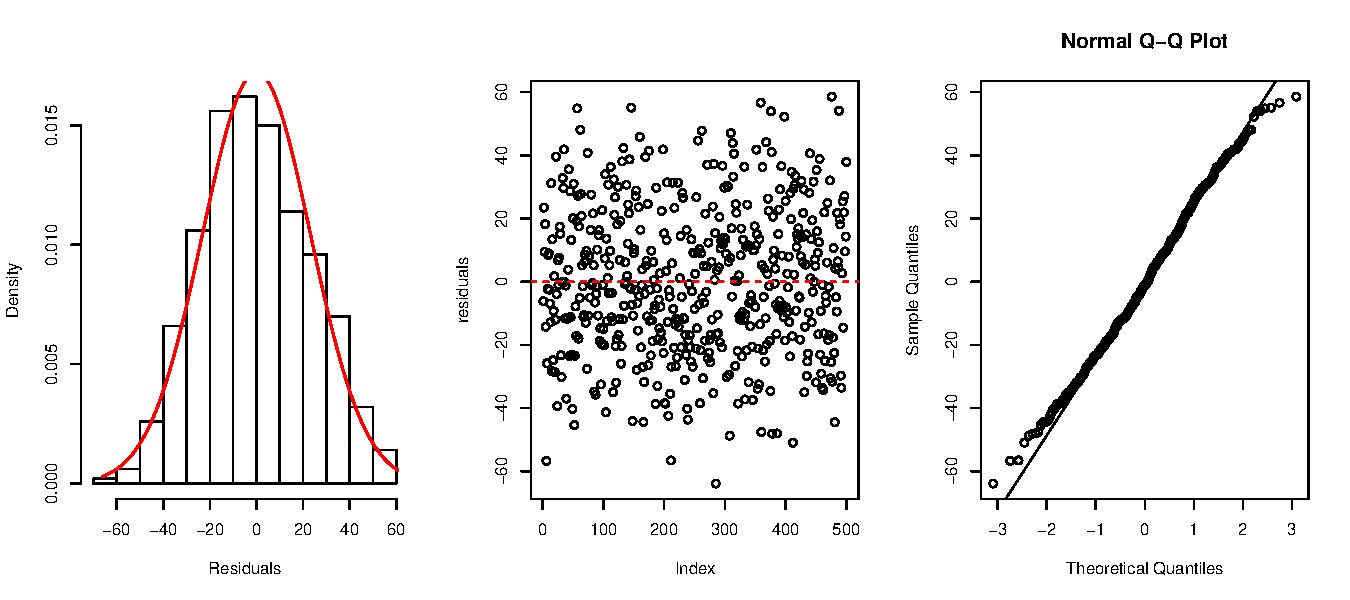
\includegraphics[width=\maxwidth]{figure/unnamed-chunk-97-1} 

}



\end{knitrout}

In the second example, the data appears somewhat normal, but with some outliers.  This does not appear to be an egregious violation, but is something that should be kept in mind as the results of the linear regression are interpreted.  

\begin{knitrout}
\definecolor{shadecolor}{rgb}{0.969, 0.969, 0.969}\color{fgcolor}\begin{kframe}
\begin{alltt}
\hlkwd{par}\hlstd{(}\hlkwc{mfrow} \hlstd{=} \hlkwd{c}\hlstd{(}\hlnum{1}\hlstd{,} \hlnum{3}\hlstd{))}
\hlcom{## Guided Practice 6.1}
\hlstd{residuals} \hlkwb{=} \hlkwd{resid}\hlstd{(}\hlkwd{lm}\hlstd{(frog.altitude.data}\hlopt{$}\hlstd{clutch.volume} \hlopt{~} \hlstd{frog.altitude.data}\hlopt{$}\hlstd{body.size))}

\hlkwd{hist}\hlstd{(residuals,} \hlkwc{main} \hlstd{=} \hlstr{""}\hlstd{,} \hlkwc{xlab} \hlstd{=} \hlstr{"Residuals"}\hlstd{,} \hlkwc{freq} \hlstd{=} \hlnum{FALSE}\hlstd{)}
\hlstd{x} \hlkwb{<-} \hlkwd{seq}\hlstd{(}\hlkwd{min}\hlstd{(residuals)} \hlopt{-} \hlnum{2}\hlstd{,} \hlkwd{max}\hlstd{(residuals)} \hlopt{+} \hlnum{2}\hlstd{,} \hlnum{0.01}\hlstd{)}
\hlstd{y} \hlkwb{<-} \hlkwd{dnorm}\hlstd{(x,} \hlkwd{mean}\hlstd{(residuals),} \hlkwd{sd}\hlstd{(residuals))}
\hlkwd{lines}\hlstd{(x, y,} \hlkwc{lwd} \hlstd{=} \hlnum{1.5}\hlstd{,} \hlkwc{col} \hlstd{=} \hlstr{"red"}\hlstd{)}

\hlkwd{plot}\hlstd{(residuals)}
\hlkwd{abline}\hlstd{(}\hlkwc{h} \hlstd{=} \hlnum{0}\hlstd{,} \hlkwc{col} \hlstd{=} \hlstr{"red"}\hlstd{,} \hlkwc{lty} \hlstd{=} \hlnum{2}\hlstd{)}

\hlkwd{qqnorm}\hlstd{(residuals)}
\hlkwd{qqline}\hlstd{(residuals)}
\end{alltt}
\end{kframe}

{\centering 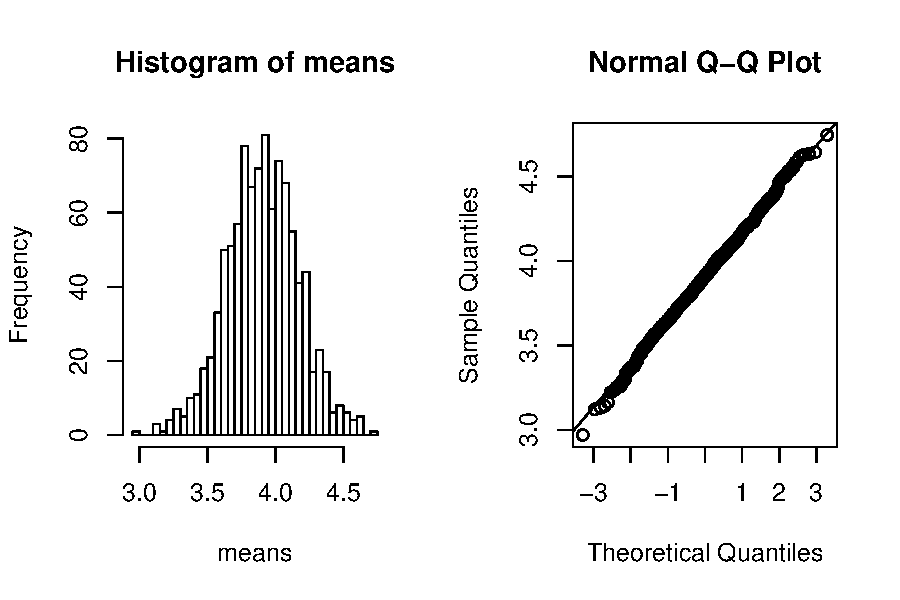
\includegraphics[width=\maxwidth]{figure/unnamed-chunk-98-1} 

}



\end{knitrout}


\section{Creating a Linear Regression}
Using $R$ to create a linear regression is quite simple, and several examples will be shown here to illustrate that.  As background, there is one command needed for linear regressions in $R$, \textit{lm()}.  This function takes two arguments, the \textbf{explanatory variable} and the \textbf{response variable} in the form \textit{lm(response} $\sim$ \textit{explanatory)} where the symbol between those two variables is a tilde.  For example, a regression for the statins data can be calculated as follows 
\begin{knitrout}
\definecolor{shadecolor}{rgb}{0.969, 0.969, 0.969}\color{fgcolor}\begin{kframe}
\begin{alltt}
\hlkwd{lm}\hlstd{(statins.samp}\hlopt{$}\hlstd{RFFT}\hlopt{~}\hlstd{statins.samp}\hlopt{$}\hlstd{Age)}
\end{alltt}
\begin{verbatim}
## 
## Call:
## lm(formula = statins.samp$RFFT ~ statins.samp$Age)
## 
## Coefficients:
##      (Intercept)  statins.samp$Age  
##          137.550            -1.261
\end{verbatim}
\end{kframe}
\end{knitrout}

This output implies the following regression formula 
\[RFFT = 137.55 - 1.261 \cdot Age\]

To get more information about the regression, the \textit{summary} command can be used as follows, 

\begin{knitrout}
\definecolor{shadecolor}{rgb}{0.969, 0.969, 0.969}\color{fgcolor}\begin{kframe}
\begin{alltt}
\hlkwd{summary}\hlstd{(}\hlkwd{lm}\hlstd{(statins.samp}\hlopt{$}\hlstd{RFFT}\hlopt{~}\hlstd{statins.samp}\hlopt{$}\hlstd{Age))}
\end{alltt}
\begin{verbatim}
## 
## Call:
## lm(formula = statins.samp$RFFT ~ statins.samp$Age)
## 
## Residuals:
##     Min      1Q  Median      3Q     Max 
## -63.879 -16.845  -1.095  15.524  58.564 
## 
## Coefficients:
##                   Estimate Std. Error t value Pr(>|t|)    
## (Intercept)      137.54972    5.01614   27.42   <2e-16 ***
## statins.samp$Age  -1.26136    0.08953  -14.09   <2e-16 ***
## ---
## Signif. codes:  0 '***' 0.001 '**' 0.01 '*' 0.05 '.' 0.1 ' ' 1
## 
## Residual standard error: 23.19 on 498 degrees of freedom
## Multiple R-squared:  0.285,	Adjusted R-squared:  0.2836 
## F-statistic: 198.5 on 1 and 498 DF,  p-value: < 2.2e-16
\end{verbatim}
\end{kframe}
\end{knitrout}
Note that the summary of the linear regression is much more useful, providing not only the regression model, but standard errors, p-values, the $R^2$ value, and a few other useful statistics which will be discussed in greater deal in future chapters.  

With this linear regression in mind, it would be helpful to be able to visualize this on the scatterplot.  This can be done using the command \textit{abline()}, which takes as its arguments the model itself.  

\begin{knitrout}
\definecolor{shadecolor}{rgb}{0.969, 0.969, 0.969}\color{fgcolor}\begin{kframe}
\begin{alltt}
\hlkwd{plot}\hlstd{(statins.samp}\hlopt{$}\hlstd{RFFT} \hlopt{~} \hlstd{statins.samp}\hlopt{$}\hlstd{Age,} \hlkwc{cex} \hlstd{=} \hlnum{0.4}\hlstd{)}
\hlkwd{abline}\hlstd{(}\hlkwd{lm}\hlstd{(statins.samp}\hlopt{$}\hlstd{RFFT} \hlopt{~} \hlstd{statins.samp}\hlopt{$}\hlstd{Age),} \hlkwc{col} \hlstd{=} \hlstr{"red"}\hlstd{)}
\end{alltt}
\end{kframe}

{\centering 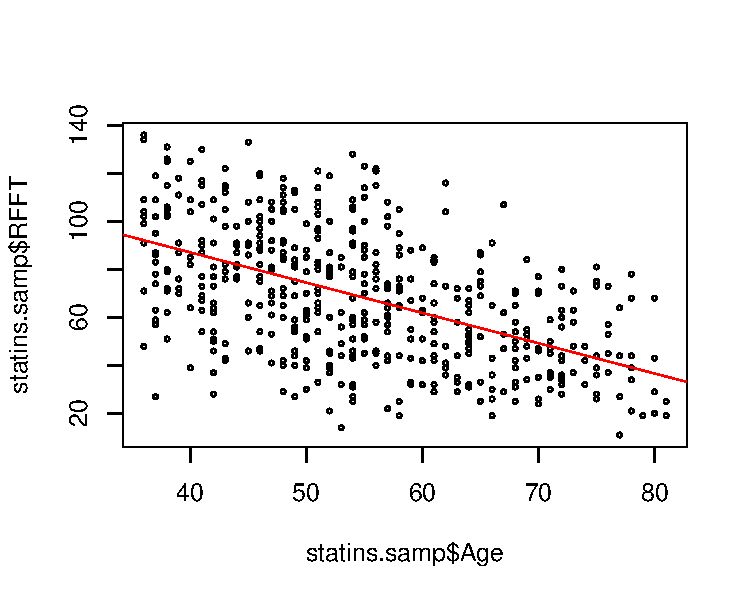
\includegraphics[width=\maxwidth]{figure/unnamed-chunk-101-1} 

}



\end{knitrout}

\subsection{FAMuSS Regression}
Performing a similar regression for the FAMuSS dataset between height and weight gives us the following model
\[ weight = -187.79 + 5.14 \cdot height \]

\begin{knitrout}
\definecolor{shadecolor}{rgb}{0.969, 0.969, 0.969}\color{fgcolor}\begin{kframe}
\begin{alltt}
\hlkwd{plot}\hlstd{(famuss}\hlopt{$}\hlstd{weight} \hlopt{~} \hlstd{famuss}\hlopt{$}\hlstd{height)}
\hlkwd{abline}\hlstd{(}\hlkwd{lm}\hlstd{(famuss}\hlopt{$}\hlstd{weight} \hlopt{~} \hlstd{famuss}\hlopt{$}\hlstd{height))}
\end{alltt}
\end{kframe}

{\centering 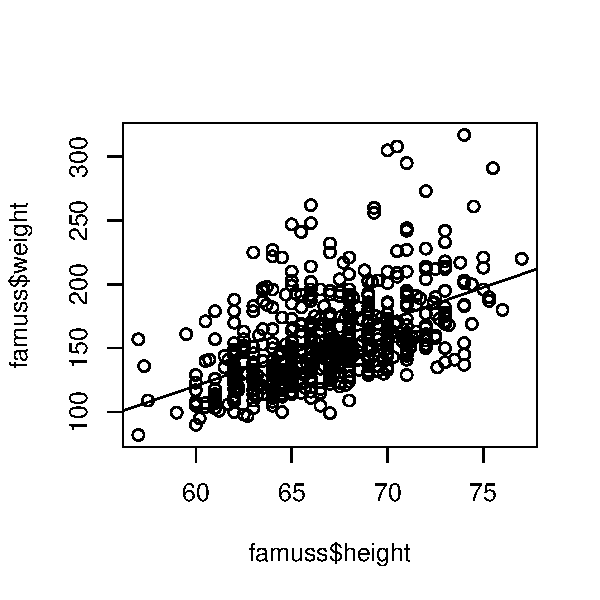
\includegraphics[width=\maxwidth]{figure/unnamed-chunk-102-1} 

}


\begin{kframe}\begin{alltt}
\hlkwd{summary}\hlstd{(}\hlkwd{lm}\hlstd{(famuss}\hlopt{$}\hlstd{weight} \hlopt{~} \hlstd{famuss}\hlopt{$}\hlstd{height))}
\end{alltt}
\begin{verbatim}
## 
## Call:
## lm(formula = famuss$weight ~ famuss$height)
## 
## Residuals:
##     Min      1Q  Median      3Q     Max 
## -57.514 -19.452  -6.959  13.882 133.500 
## 
## Coefficients:
##                Estimate Std. Error t value Pr(>|t|)    
## (Intercept)   -187.7908    22.5454  -8.329 5.64e-16 ***
## famuss$height    5.1389     0.3369  15.255  < 2e-16 ***
## ---
## Signif. codes:  0 '***' 0.001 '**' 0.01 '*' 0.05 '.' 0.1 ' ' 1
## 
## Residual standard error: 29.34 on 593 degrees of freedom
## Multiple R-squared:  0.2818,	Adjusted R-squared:  0.2806 
## F-statistic: 232.7 on 1 and 593 DF,  p-value: < 2.2e-16
\end{verbatim}
\end{kframe}
\end{knitrout}

\subsection{WDI Regression with Two Levels}
Although the interpretation of such a model can be different, the method of performing a regression on a variable with two levels is the same.  The command below illustrates how to obtain Table 6.16.  
\begin{knitrout}
\definecolor{shadecolor}{rgb}{0.969, 0.969, 0.969}\color{fgcolor}\begin{kframe}
\begin{alltt}
\hlkwd{summary}\hlstd{(}\hlkwd{lm}\hlstd{(}\hlkwd{log}\hlstd{(wdi.2011}\hlopt{$}\hlstd{inf.mort)}\hlopt{~}\hlstd{wdi.2011}\hlopt{$}\hlstd{sanit.access.factor))}
\end{alltt}
\begin{verbatim}
## 
## Call:
## lm(formula = log(wdi.2011$inf.mort) ~ wdi.2011$sanit.access.factor)
## 
## Residuals:
##     Min      1Q  Median      3Q     Max 
## -1.7501 -0.4829  0.0440  0.4407  2.0008 
## 
## Coefficients:
##                                  Estimate Std. Error t value Pr(>|t|)    
## (Intercept)                        4.0184     0.1100   36.52   <2e-16 ***
## wdi.2011$sanit.access.factorhigh  -1.6806     0.1322  -12.72   <2e-16 ***
## ---
## Signif. codes:  0 '***' 0.001 '**' 0.01 '*' 0.05 '.' 0.1 ' ' 1
## 
## Residual standard error: 0.7781 on 161 degrees of freedom
##   (2 observations deleted due to missingness)
## Multiple R-squared:  0.5011,	Adjusted R-squared:  0.498 
## F-statistic: 161.7 on 1 and 161 DF,  p-value: < 2.2e-16
\end{verbatim}
\end{kframe}
\end{knitrout}

Furthermore, the two t-tests shown in the text can be computed as follows.  Note that the first t-test, which assumes an equal variance among groups, gives the same t-statistic and p-value as the regression above.  
\begin{knitrout}
\definecolor{shadecolor}{rgb}{0.969, 0.969, 0.969}\color{fgcolor}\begin{kframe}
\begin{alltt}
\hlcom{## Pooled t-test }
\hlkwd{t.test}\hlstd{(}\hlkwd{log}\hlstd{(wdi.2011}\hlopt{$}\hlstd{inf.mort)}\hlopt{~}\hlstd{wdi.2011}\hlopt{$}\hlstd{sanit.access.factor,} \hlkwc{var.equal} \hlstd{=} \hlnum{TRUE}\hlstd{)}
\end{alltt}
\begin{verbatim}
## 
## 	Two Sample t-test
## 
## data:  log(wdi.2011$inf.mort) by wdi.2011$sanit.access.factor
## t = 12.7166, df = 161, p-value < 2.2e-16
## alternative hypothesis: true difference in means is not equal to 0
## 95 percent confidence interval:
##  1.419601 1.941570
## sample estimates:
##  mean in group low mean in group high 
##           4.018421           2.337835
\end{verbatim}
\begin{alltt}
\hlcom{## Unpooled t-test }
\hlkwd{t.test}\hlstd{(}\hlkwd{log}\hlstd{(wdi.2011}\hlopt{$}\hlstd{inf.mort)}\hlopt{~}\hlstd{wdi.2011}\hlopt{$}\hlstd{sanit.access.factor,} \hlkwc{var.equal} \hlstd{=} \hlnum{TRUE}\hlstd{)}
\end{alltt}
\begin{verbatim}
## 
## 	Two Sample t-test
## 
## data:  log(wdi.2011$inf.mort) by wdi.2011$sanit.access.factor
## t = 12.7166, df = 161, p-value < 2.2e-16
## alternative hypothesis: true difference in means is not equal to 0
## 95 percent confidence interval:
##  1.419601 1.941570
## sample estimates:
##  mean in group low mean in group high 
##           4.018421           2.337835
\end{verbatim}
\end{kframe}
\end{knitrout}



\newpage
\chapter{Multiple Linear Regression}
\minitoc


%% FIGURE NUMBERs WILL LIKELY CHANGE WHEN CH 7 IS FINALIZED, SO CHECK THEM ALL AT SOME POINT 

In Chapter 6, the dataset \textit{statins} was introduced when visually understanding the assumptions of simple linear regression.  It will again be used in this chapter to understand the idea of multiple linear regression.

%% Should I include Figure 7.2 in here, seems uneccessary.  

\section*{Confounders} 

\begin{knitrout}
\definecolor{shadecolor}{rgb}{0.969, 0.969, 0.969}\color{fgcolor}\begin{kframe}
\begin{alltt}
\hlcom{## Figure 7.1 First collecting the data sample}
\hlkwd{set.seed}\hlstd{(}\hlnum{5011}\hlstd{)}
\hlstd{row.num} \hlkwb{=} \hlkwd{sample}\hlstd{(}\hlnum{1}\hlopt{:}\hlkwd{nrow}\hlstd{(statins),} \hlnum{500}\hlstd{,} \hlkwc{replace} \hlstd{=} \hlnum{FALSE}\hlstd{)}
\hlstd{statins.samp} \hlkwb{=} \hlstd{statins[row.num, ]}

\hlcom{# Make the plot where color is specified by Statin use}
\hlkwd{plot}\hlstd{(statins.samp}\hlopt{$}\hlstd{Age, statins.samp}\hlopt{$}\hlstd{RFFT,} \hlkwc{pch} \hlstd{=} \hlnum{19}\hlstd{,} \hlkwc{cex} \hlstd{=} \hlnum{1.3}\hlstd{,} \hlkwc{col} \hlstd{=} \hlkwd{as.factor}\hlstd{(statins.samp}\hlopt{$}\hlstd{Statin),}
    \hlkwc{xlab} \hlstd{=} \hlstr{"Age (yrs)"}\hlstd{,} \hlkwc{ylab} \hlstd{=} \hlstr{"RFFT Score"}\hlstd{)}
\end{alltt}
\end{kframe}

{\centering 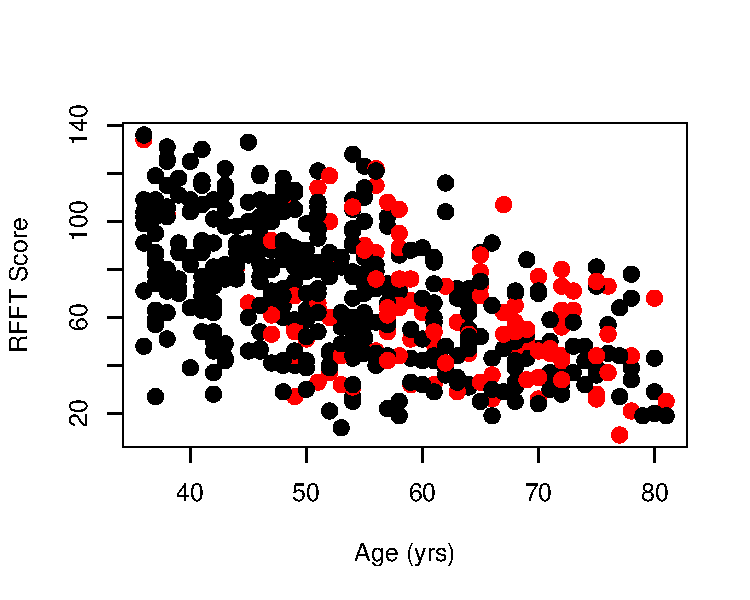
\includegraphics[width=\maxwidth]{figure/unnamed-chunk-105-1} 

}



\end{knitrout}

The text walks through the example of statin use as being a confounder because it is theoretically associated with both another explanatory variable, in this case age, and response variable, here cognitive decline.  To test for a confounder, a measure of association can be used such as correlation or a side-by-side boxplot.  In this example, the correlations between the variables can be calculated as follows.  

\begin{knitrout}
\definecolor{shadecolor}{rgb}{0.969, 0.969, 0.969}\color{fgcolor}\begin{kframe}
\begin{alltt}
\hlcom{## Figure 7.4 Visual test of association}
\hlkwd{boxplot}\hlstd{(statins.samp}\hlopt{$}\hlstd{Age} \hlopt{~} \hlstd{statins.samp}\hlopt{$}\hlstd{Statin,} \hlkwc{ylab} \hlstd{=} \hlstr{"Age (yrs)"}\hlstd{,} \hlkwc{xlab} \hlstd{=} \hlstr{"Statin Use"}\hlstd{)}
\end{alltt}
\end{kframe}

{\centering 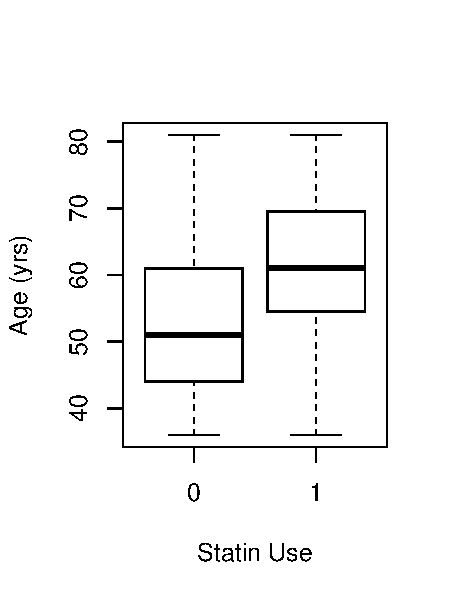
\includegraphics[width=\maxwidth]{figure/unnamed-chunk-106-1} 

}


\begin{kframe}\begin{alltt}
\hlcom{# Numerical test of association}
\hlkwd{cor}\hlstd{(statins.samp}\hlopt{$}\hlstd{Statin, statins.samp}\hlopt{$}\hlstd{Age)}
\end{alltt}
\begin{verbatim}
## [1] 0.3116923
\end{verbatim}
\begin{alltt}
\hlkwd{cor}\hlstd{(statins.samp}\hlopt{$}\hlstd{Statin, statins.samp}\hlopt{$}\hlstd{RFFT)}
\end{alltt}
\begin{verbatim}
## [1] -0.1545881
\end{verbatim}
\end{kframe}
\end{knitrout}

A correlation greater than 0.3 or less than -0.3 is considered signficant.  Note that these correlations are not immediately concerning as only one is mildly signficant, but nonetheless, they could be impactful on an investigation and should be accounted for if possible.  The conclusion in the main text is thus that a multiple linear regression should be used because it can adjust for confounders.  The explanation of how this works is complicated, but the idea is that because multiple linear regression builds a model that reflects the association between explanatory and response variables, the more information included in building this model, the better.  

\stepcounter{section}
\section{Simple vs. Multiple Regression}
Firstly, the simple linear regression can be performed as would have been done in Chapter 6.  
\begin{knitrout}
\definecolor{shadecolor}{rgb}{0.969, 0.969, 0.969}\color{fgcolor}\begin{kframe}
\begin{alltt}
\hlkwd{summary}\hlstd{(}\hlkwd{lm}\hlstd{(statins.samp}\hlopt{$}\hlstd{RFFT} \hlopt{~} \hlstd{statins.samp}\hlopt{$}\hlstd{Statin))}
\end{alltt}
\begin{verbatim}
## 
## Call:
## lm(formula = statins.samp$RFFT ~ statins.samp$Statin)
## 
## Residuals:
##     Min      1Q  Median      3Q     Max 
## -56.714 -22.714   0.286  18.299  73.339 
## 
## Coefficients:
##                     Estimate Std. Error t value Pr(>|t|)    
## (Intercept)           70.714      1.381  51.212  < 2e-16 ***
## statins.samp$Statin  -10.053      2.879  -3.492 0.000523 ***
## ---
## Signif. codes:  0 '***' 0.001 '**' 0.01 '*' 0.05 '.' 0.1 ' ' 1
## 
## Residual standard error: 27.09 on 498 degrees of freedom
## Multiple R-squared:  0.0239,	Adjusted R-squared:  0.02194 
## F-statistic: 12.19 on 1 and 498 DF,  p-value: 0.0005226
\end{verbatim}
\end{kframe}
\end{knitrout}
This gives the following model, 
\[ RFFT = 70.714 - 10.053\cdot Statin \]

Next, the multiple regression will be performed. Note the use of a plus sign after the tilde to include multiple variables.   
\begin{knitrout}
\definecolor{shadecolor}{rgb}{0.969, 0.969, 0.969}\color{fgcolor}\begin{kframe}
\begin{alltt}
\hlkwd{summary}\hlstd{(}\hlkwd{lm}\hlstd{(statins.samp}\hlopt{$}\hlstd{RFFT} \hlopt{~} \hlstd{statins.samp}\hlopt{$}\hlstd{Statin} \hlopt{+} \hlstd{statins.samp}\hlopt{$}\hlstd{Age))}
\end{alltt}
\begin{verbatim}
## 
## Call:
## lm(formula = statins.samp$RFFT ~ statins.samp$Statin + statins.samp$Age)
## 
## Residuals:
##     Min      1Q  Median      3Q     Max 
## -63.855 -16.860  -1.178  15.730  58.751 
## 
## Coefficients:
##                     Estimate Std. Error t value Pr(>|t|)    
## (Intercept)         137.8822     5.1221  26.919   <2e-16 ***
## statins.samp$Statin   0.8509     2.5957   0.328    0.743    
## statins.samp$Age     -1.2710     0.0943 -13.478   <2e-16 ***
## ---
## Signif. codes:  0 '***' 0.001 '**' 0.01 '*' 0.05 '.' 0.1 ' ' 1
## 
## Residual standard error: 23.21 on 497 degrees of freedom
## Multiple R-squared:  0.2852,	Adjusted R-squared:  0.2823 
## F-statistic: 99.13 on 2 and 497 DF,  p-value: < 2.2e-16
\end{verbatim}
\end{kframe}
\end{knitrout}
This gives the following model, 
\[ RFFT = 137.8822 + 0.8509\cdot Statin - 1.2710 \cdot Age\]

As compared to a model with statin use as the only explanatory variable, it is evident that the coefficients here change quite drastically by including both explanatory variables.  This is reflective of the confounding relationship between the two explanatory variables, but will hopefully lead us to more accurate results.  

Notice how in this example, the first model shows a negative relationship between statin use and RFFT values, while the multiple regression shows a positive relationship.  This is reflective that the \textit{Statin} variable is representative of different things in the two models.  In the simple model, the coefficient for statin use represents the difference between the mean of RFFT value for the two groups, statin users and non-users.  This calculation can be seen directly from the sample below.  However, the coefficient in the multiple regression model is significantly more complicated.  It represents the average difference in means for statin users and non-users of the same age.  

\begin{knitrout}
\definecolor{shadecolor}{rgb}{0.969, 0.969, 0.969}\color{fgcolor}\begin{kframe}
\begin{alltt}
\hlcom{# Calculation of the simple linear regression coefficient}
\hlkwd{mean}\hlstd{(statins.samp}\hlopt{$}\hlstd{RFFT[statins.samp}\hlopt{$}\hlstd{Statin} \hlopt{==} \hlnum{1}\hlstd{])} \hlopt{-} \hlkwd{mean}\hlstd{(statins.samp}\hlopt{$}\hlstd{RFFT[statins.samp}\hlopt{$}\hlstd{Statin} \hlopt{==} \hlnum{0}\hlstd{])}
\end{alltt}
\begin{verbatim}
## [1] -10.05342
\end{verbatim}
\end{kframe}
\end{knitrout}


\section{Evaluating The Fit of a Multiple Regression Model}
\subsection{Assumptions of Linear Regression}
The same procedures as outlined in Chapter 6 can be used to test the model assumptions, and will be repeated here.  
\begin{enumerate}
\item \textbf{Linearity:}  The plots below show that the relationship of the response variable with each explanatory variable is approximately linear.    
\begin{knitrout}
\definecolor{shadecolor}{rgb}{0.969, 0.969, 0.969}\color{fgcolor}\begin{kframe}
\begin{alltt}
\hlkwd{par}\hlstd{(}\hlkwc{mfrow} \hlstd{=} \hlkwd{c}\hlstd{(}\hlnum{1}\hlstd{,} \hlnum{2}\hlstd{))}
\hlkwd{plot}\hlstd{(statins.samp}\hlopt{$}\hlstd{RFFT} \hlopt{~} \hlstd{statins.samp}\hlopt{$}\hlstd{Age,} \hlkwc{cex} \hlstd{=} \hlnum{0.6}\hlstd{,} \hlkwc{ylab} \hlstd{=} \hlstr{"RFFT Score"}\hlstd{,} \hlkwc{xlab} \hlstd{=} \hlstr{"Age (yrs)"}\hlstd{,}
    \hlkwc{main} \hlstd{=} \hlstr{""}\hlstd{)}
\hlkwd{abline}\hlstd{(}\hlkwd{lm}\hlstd{(statins.samp}\hlopt{$}\hlstd{RFFT} \hlopt{~} \hlstd{statins.samp}\hlopt{$}\hlstd{Age),} \hlkwc{col} \hlstd{=} \hlstr{"red"}\hlstd{)}
\hlkwd{plot}\hlstd{(statins.samp}\hlopt{$}\hlstd{RFFT} \hlopt{~} \hlstd{statins.samp}\hlopt{$}\hlstd{Statin,} \hlkwc{cex} \hlstd{=} \hlnum{0.6}\hlstd{,} \hlkwc{ylab} \hlstd{=} \hlstr{"RFFT Score"}\hlstd{,}
    \hlkwc{xlab} \hlstd{=} \hlstr{"Age (yrs)"}\hlstd{,} \hlkwc{main} \hlstd{=} \hlstr{""}\hlstd{)}
\hlkwd{abline}\hlstd{(}\hlkwd{lm}\hlstd{(statins.samp}\hlopt{$}\hlstd{RFFT} \hlopt{~} \hlstd{statins.samp}\hlopt{$}\hlstd{Statin),} \hlkwc{col} \hlstd{=} \hlstr{"red"}\hlstd{)}
\end{alltt}
\end{kframe}

{\centering 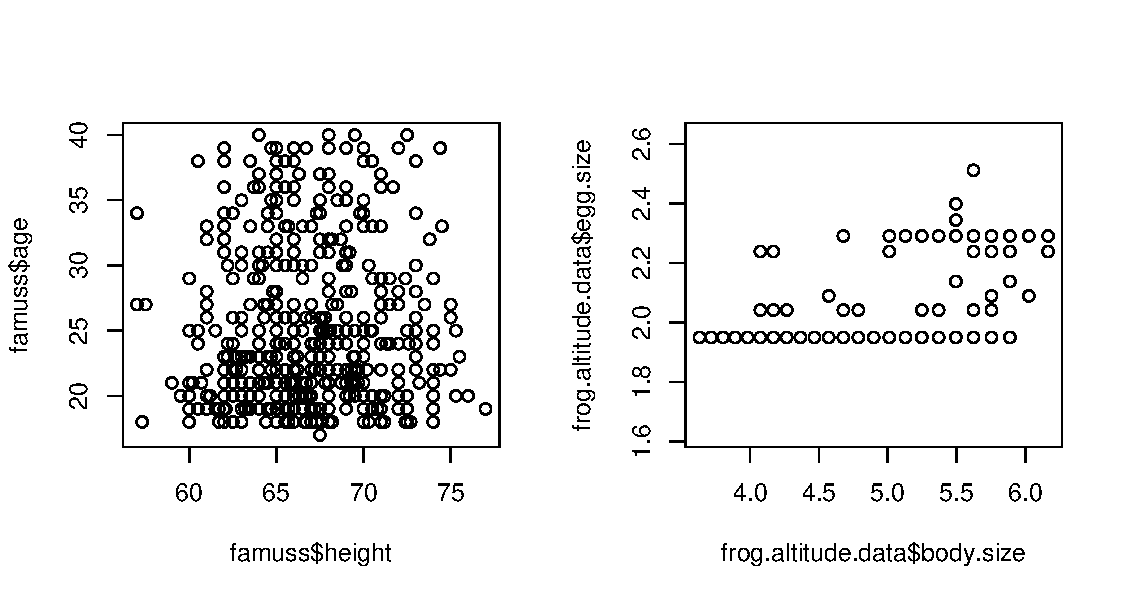
\includegraphics[width=\maxwidth]{figure/unnamed-chunk-110-1} 

}



\end{knitrout}

\item \textbf{Constant Variability:} Note that the assumption is approximately constant variance in the \textit{residuals}, which can be investigated with the following, showing that the residuals do appear to have constant variance.  
\begin{knitrout}
\definecolor{shadecolor}{rgb}{0.969, 0.969, 0.969}\color{fgcolor}\begin{kframe}
\begin{alltt}
\hlstd{residuals} \hlkwb{=} \hlkwd{resid}\hlstd{(}\hlkwd{lm}\hlstd{(statins.samp}\hlopt{$}\hlstd{RFFT} \hlopt{~} \hlstd{statins.samp}\hlopt{$}\hlstd{Age} \hlopt{+} \hlstd{statins.samp}\hlopt{$}\hlstd{Statin))}
\hlkwd{plot}\hlstd{(residuals,} \hlkwc{ylab} \hlstd{=} \hlstr{"Residuals"}\hlstd{)}
\end{alltt}
\end{kframe}

{\centering 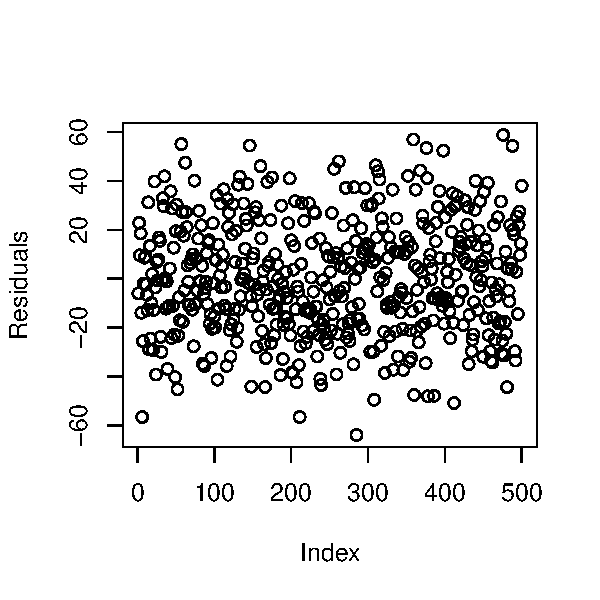
\includegraphics[width=\maxwidth]{figure/unnamed-chunk-111-1} 

}



\end{knitrout}

\item \textbf{Independent Observations:} This assumption remains dependent on the data collection itself, and based on the parameters of the study, the data is believed to be independent.  

\item \textbf{Residuals that are approximately normally distributed:} This can be investigated with a historgram or a normal q-q plot as follows.  The residuals do appear to be approximately normally distributed.  
\begin{knitrout}
\definecolor{shadecolor}{rgb}{0.969, 0.969, 0.969}\color{fgcolor}\begin{kframe}
\begin{alltt}
\hlkwd{par}\hlstd{(}\hlkwc{mfrow} \hlstd{=} \hlkwd{c}\hlstd{(}\hlnum{1}\hlstd{,} \hlnum{2}\hlstd{))}
\hlkwd{hist}\hlstd{(residuals,} \hlkwc{xlab} \hlstd{=} \hlstr{"Residuals"}\hlstd{,} \hlkwc{freq} \hlstd{=} \hlnum{FALSE}\hlstd{)}
\hlstd{x} \hlkwb{<-} \hlkwd{seq}\hlstd{(}\hlkwd{min}\hlstd{(residuals)} \hlopt{-} \hlnum{2}\hlstd{,} \hlkwd{max}\hlstd{(residuals)} \hlopt{+} \hlnum{2}\hlstd{,} \hlnum{0.01}\hlstd{)}
\hlstd{y} \hlkwb{<-} \hlkwd{dnorm}\hlstd{(x,} \hlkwd{mean}\hlstd{(residuals),} \hlkwd{sd}\hlstd{(residuals))}
\hlkwd{lines}\hlstd{(x, y,} \hlkwc{lwd} \hlstd{=} \hlnum{1.5}\hlstd{,} \hlkwc{col} \hlstd{=} \hlstr{"red"}\hlstd{)}

\hlkwd{qqnorm}\hlstd{(residuals)}
\hlkwd{qqline}\hlstd{(residuals)}
\end{alltt}
\end{kframe}

{\centering 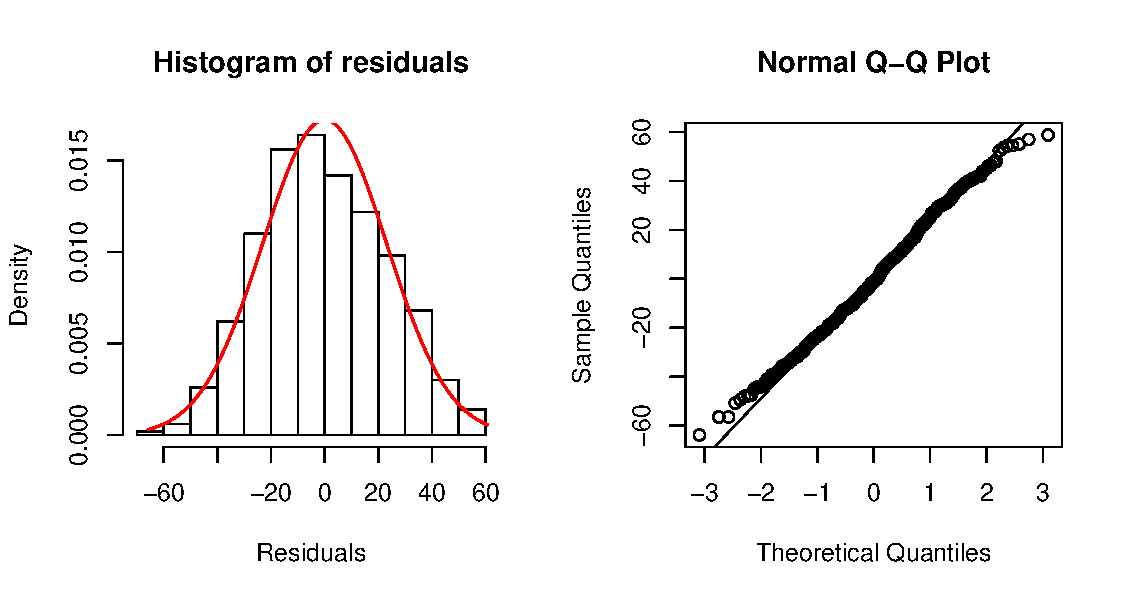
\includegraphics[width=\maxwidth]{figure/unnamed-chunk-112-1} 

}



\end{knitrout}

\end{enumerate}

\subsection{Hypothesis Tests and Confidence Intervals}
$R$ makes the process of performing hypothesis tests on coefficients of the multiple linear regression model very simple, as it performs all the tests and automatically returns these in the summary of the linear regression.  As with simple linear regression, the $R$ output of a multiple regression provides a t-statistic and a corresponding p-value for the hypothesis test of 
\[ H_0: \beta_k = 0 \text{vs. } H_A: \beta_k \neq 0 \]

Furthermore, the summary output also includes the F-statistic for the hypothesis 
\[ H_0: \beta_1 = \beta_2 = \cdots = \beta_p = 0 \]
In words, this tests if any of the coefficients in combination are useful at predicting the response variable.  Note that this tests if any of the coefficients is non-zero, not if all of them are non-zero.  

\stepcounter{section}
\section{Categorical Predictors With More Than Two Values}
The function \textit{as.factor()} has previously been used to tell $R$ to treat the numerical values of a variable as frivolous, rather representing different categories.  In other words, a value of 1 for statin does not imply one unit of statins were used by the individual, rather that any amount of statins were used.  Data is often stored with numerical values for ease of manipulation, even if the numerical values do not have significant meaning.  In these cases, it is important to utilize the function \textit{as.factor()} to clarify to $R$ whether the numbers have meaning as numbers or as categories, with \textit{as.factor()} implying that they are categories, or factors.  

Using this idea on the statin sample data, the following simple regression is obtained, with the reference category being a value of 0 for \textit{Statin} since it is the one that is not printed in the output.  
\begin{knitrout}
\definecolor{shadecolor}{rgb}{0.969, 0.969, 0.969}\color{fgcolor}\begin{kframe}
\begin{alltt}
\hlkwd{summary}\hlstd{(}\hlkwd{lm}\hlstd{(statins.samp}\hlopt{$}\hlstd{RFFT} \hlopt{~} \hlkwd{as.factor}\hlstd{(statins.samp}\hlopt{$}\hlstd{Statin)))}
\end{alltt}
\begin{verbatim}
## 
## Call:
## lm(formula = statins.samp$RFFT ~ as.factor(statins.samp$Statin))
## 
## Residuals:
##     Min      1Q  Median      3Q     Max 
## -56.714 -22.714   0.286  18.299  73.339 
## 
## Coefficients:
##                                 Estimate Std. Error t value Pr(>|t|)    
## (Intercept)                       70.714      1.381  51.212  < 2e-16 ***
## as.factor(statins.samp$Statin)1  -10.053      2.879  -3.492 0.000523 ***
## ---
## Signif. codes:  0 '***' 0.001 '**' 0.01 '*' 0.05 '.' 0.1 ' ' 1
## 
## Residual standard error: 27.09 on 498 degrees of freedom
## Multiple R-squared:  0.0239,	Adjusted R-squared:  0.02194 
## F-statistic: 12.19 on 1 and 498 DF,  p-value: 0.0005226
\end{verbatim}
\end{kframe}
\end{knitrout}
In this example, the regression using \textit{Statin} as either a numerical value or as a categorical variable is the same because of the method by which it was encoded.  Using binary values, i.e. 0 and 1, signals to $R$ that a variable is a categorical variable, and this is mathematically equivalent.  Where this becomes significantly more complicated is when there are more than two categories because $R$ can no longer make the assumption of categorical variable and will assume non-categorical values with numerical significance.  

An example of where this is a problem is as follows, 
\begin{knitrout}
\definecolor{shadecolor}{rgb}{0.969, 0.969, 0.969}\color{fgcolor}\begin{kframe}
\begin{alltt}
\hlcom{## NOTE, this method is INCORRECT and provided for example,}
\hlcom{## so please be careful copying }
\hlkwd{summary}\hlstd{(}\hlkwd{lm}\hlstd{(statins.samp}\hlopt{$}\hlstd{RFFT} \hlopt{~} \hlstd{statins.samp}\hlopt{$}\hlstd{Education))}
\end{alltt}
\begin{verbatim}
## 
## Call:
## lm(formula = statins.samp$RFFT ~ statins.samp$Education)
## 
## Residuals:
##     Min      1Q  Median      3Q     Max 
## -56.622 -16.148  -0.885  15.536  62.694 
## 
## Coefficients:
##                        Estimate Std. Error t value Pr(>|t|)    
## (Intercept)              41.148      2.104   19.55   <2e-16 ***
## statins.samp$Education   15.158      1.023   14.81   <2e-16 ***
## ---
## Signif. codes:  0 '***' 0.001 '**' 0.01 '*' 0.05 '.' 0.1 ' ' 1
## 
## Residual standard error: 22.85 on 498 degrees of freedom
## Multiple R-squared:  0.3059,	Adjusted R-squared:  0.3045 
## F-statistic: 219.5 on 1 and 498 DF,  p-value: < 2.2e-16
\end{verbatim}
\begin{alltt}
\hlcom{## Correct method }
\hlkwd{summary}\hlstd{(}\hlkwd{lm}\hlstd{(statins.samp}\hlopt{$}\hlstd{RFFT} \hlopt{~} \hlkwd{as.factor}\hlstd{(statins.samp}\hlopt{$}\hlstd{Education)))}
\end{alltt}
\begin{verbatim}
## 
## Call:
## lm(formula = statins.samp$RFFT ~ as.factor(statins.samp$Education))
## 
## Residuals:
##     Min      1Q  Median      3Q     Max 
## -55.905 -15.975  -0.905  16.068  63.280 
## 
## Coefficients:
##                                    Estimate Std. Error t value Pr(>|t|)
## (Intercept)                          40.941      3.203  12.783  < 2e-16
## as.factor(statins.samp$Education)1   14.779      3.686   4.009 7.04e-05
## as.factor(statins.samp$Education)2   32.133      3.763   8.539  < 2e-16
## as.factor(statins.samp$Education)3   44.964      3.684  12.207  < 2e-16
##                                       
## (Intercept)                        ***
## as.factor(statins.samp$Education)1 ***
## as.factor(statins.samp$Education)2 ***
## as.factor(statins.samp$Education)3 ***
## ---
## Signif. codes:  0 '***' 0.001 '**' 0.01 '*' 0.05 '.' 0.1 ' ' 1
## 
## Residual standard error: 22.87 on 496 degrees of freedom
## Multiple R-squared:  0.3072,	Adjusted R-squared:  0.303 
## F-statistic:  73.3 on 3 and 496 DF,  p-value: < 2.2e-16
\end{verbatim}
\end{kframe}
\end{knitrout}

Notice that for an individual with an education level of 2, the first \textit{incorrect} model predicts an RFFT score of 71.464 while the second \textit{correct} model predicts a score of 73.1074.  In this example, the difference is not massive but certainly of concern, so use serious caution when working with categorical variables in $R$.  

\subsection{Using ANOVA For Categorical Variables}
When using the ANOVA for categorical variables, it is important to keep in mind that they must again be treated correctly as factors and not as numerical values.  An example of the above model treated using an ANOVA is given below.  
\begin{knitrout}
\definecolor{shadecolor}{rgb}{0.969, 0.969, 0.969}\color{fgcolor}\begin{kframe}
\begin{alltt}
\hlkwd{anova}\hlstd{(}\hlkwd{lm}\hlstd{(statins.samp}\hlopt{$}\hlstd{RFFT} \hlopt{~} \hlkwd{as.factor}\hlstd{(statins.samp}\hlopt{$}\hlstd{Education)))}
\end{alltt}
\begin{verbatim}
## Analysis of Variance Table
## 
## Response: statins.samp$RFFT
##                                    Df Sum Sq Mean Sq F value    Pr(>F)    
## as.factor(statins.samp$Education)   3 115041   38347  73.304 < 2.2e-16 ***
## Residuals                         496 259469     523                      
## ---
## Signif. codes:  0 '***' 0.001 '**' 0.01 '*' 0.05 '.' 0.1 ' ' 1
\end{verbatim}
\end{kframe}
\end{knitrout}

\subsection{Using Dummy Variables} 
Another method for considering categorical variables is the use of a dummy variable, which is a binary indicator if a value is equal to another.  In other words, a model can use several dummy variables, each of which represents a category and is equal to 1 if that individual is in the specified category and 0 otherwise.  This can be performed as follow, where the categorical value which is not seprataly specified is the reference variable.  Note that this method gives the same results as the linear regression above using \textit{as.factor()} 

\begin{knitrout}
\definecolor{shadecolor}{rgb}{0.969, 0.969, 0.969}\color{fgcolor}\begin{kframe}
\begin{alltt}
\hlstd{ed.dummy.1} \hlkwb{=} \hlstd{statins.samp}\hlopt{$}\hlstd{Education} \hlopt{==} \hlnum{1}
\hlstd{ed.dummy.2} \hlkwb{=} \hlstd{statins.samp}\hlopt{$}\hlstd{Education} \hlopt{==} \hlnum{2}
\hlstd{ed.dummy.3} \hlkwb{=} \hlstd{statins.samp}\hlopt{$}\hlstd{Education} \hlopt{==} \hlnum{3}
\hlkwd{summary}\hlstd{(}\hlkwd{lm}\hlstd{(statins.samp}\hlopt{$}\hlstd{RFFT} \hlopt{~} \hlstd{ed.dummy.1} \hlopt{+} \hlstd{ed.dummy.2} \hlopt{+} \hlstd{ed.dummy.3))}
\end{alltt}
\begin{verbatim}
## 
## Call:
## lm(formula = statins.samp$RFFT ~ ed.dummy.1 + ed.dummy.2 + ed.dummy.3)
## 
## Residuals:
##     Min      1Q  Median      3Q     Max 
## -55.905 -15.975  -0.905  16.068  63.280 
## 
## Coefficients:
##                Estimate Std. Error t value Pr(>|t|)    
## (Intercept)      40.941      3.203  12.783  < 2e-16 ***
## ed.dummy.1TRUE   14.779      3.686   4.009 7.04e-05 ***
## ed.dummy.2TRUE   32.133      3.763   8.539  < 2e-16 ***
## ed.dummy.3TRUE   44.964      3.684  12.207  < 2e-16 ***
## ---
## Signif. codes:  0 '***' 0.001 '**' 0.01 '*' 0.05 '.' 0.1 ' ' 1
## 
## Residual standard error: 22.87 on 496 degrees of freedom
## Multiple R-squared:  0.3072,	Adjusted R-squared:  0.303 
## F-statistic:  73.3 on 3 and 496 DF,  p-value: < 2.2e-16
\end{verbatim}
\end{kframe}
\end{knitrout}

\section{Analysis of the Statin Dataset}
Performing the more complex multiple regression can be done as follows, 
\begin{knitrout}
\definecolor{shadecolor}{rgb}{0.969, 0.969, 0.969}\color{fgcolor}\begin{kframe}
\begin{alltt}
\hlkwd{summary}\hlstd{(}\hlkwd{lm}\hlstd{(statins.samp}\hlopt{$}\hlstd{RFFT} \hlopt{~} \hlkwd{as.factor}\hlstd{(statins.samp}\hlopt{$}\hlstd{Statin)} \hlopt{+} \hlstd{statins.samp}\hlopt{$}\hlstd{Age} \hlopt{+} \hlkwd{as.factor}\hlstd{(statins.samp}\hlopt{$}\hlstd{Education)} \hlopt{+} \hlkwd{as.factor}\hlstd{(statins.samp}\hlopt{$}\hlstd{CVD)))}
\end{alltt}
\begin{verbatim}
## 
## Call:
## lm(formula = statins.samp$RFFT ~ as.factor(statins.samp$Statin) + 
##     statins.samp$Age + as.factor(statins.samp$Education) + as.factor(statins.samp$CVD))
## 
## Residuals:
##     Min      1Q  Median      3Q     Max 
## -56.348 -15.586  -0.136  13.795  63.935 
## 
## Coefficients:
##                                    Estimate Std. Error t value Pr(>|t|)
## (Intercept)                        99.03507    6.33012  15.645  < 2e-16
## as.factor(statins.samp$Statin)1     4.69045    2.44802   1.916  0.05594
## statins.samp$Age                   -0.92029    0.09041 -10.179  < 2e-16
## as.factor(statins.samp$Education)1 10.08831    3.37556   2.989  0.00294
## as.factor(statins.samp$Education)2 21.30146    3.57768   5.954 4.98e-09
## as.factor(statins.samp$Education)3 33.12464    3.54710   9.339  < 2e-16
## as.factor(statins.samp$CVD)1       -7.56655    3.65164  -2.072  0.03878
##                                       
## (Intercept)                        ***
## as.factor(statins.samp$Statin)1    .  
## statins.samp$Age                   ***
## as.factor(statins.samp$Education)1 ** 
## as.factor(statins.samp$Education)2 ***
## as.factor(statins.samp$Education)3 ***
## as.factor(statins.samp$CVD)1       *  
## ---
## Signif. codes:  0 '***' 0.001 '**' 0.01 '*' 0.05 '.' 0.1 ' ' 1
## 
## Residual standard error: 20.71 on 493 degrees of freedom
## Multiple R-squared:  0.4355,	Adjusted R-squared:  0.4286 
## F-statistic: 63.38 on 6 and 493 DF,  p-value: < 2.2e-16
\end{verbatim}
\end{kframe}
\end{knitrout}

Testing the assumptions and evaluating the fit, the model is reasonably good, but by no means perfect.  The $R^2$ value is only 0.4355, which is an improvement, and the plots below show fairly normal residuals. Note that a perfect model would be highly suspcious because of the nature of data analysis, so the goal is to find the best model possible without finding something suspicious.  
\begin{knitrout}
\definecolor{shadecolor}{rgb}{0.969, 0.969, 0.969}\color{fgcolor}\begin{kframe}
\begin{alltt}
\hlstd{residuals} \hlkwb{=} \hlkwd{resid}\hlstd{(}\hlkwd{lm}\hlstd{(statins.samp}\hlopt{$}\hlstd{RFFT} \hlopt{~} \hlkwd{as.factor}\hlstd{(statins.samp}\hlopt{$}\hlstd{Statin)} \hlopt{+} \hlstd{statins.samp}\hlopt{$}\hlstd{Age} \hlopt{+}
    \hlkwd{as.factor}\hlstd{(statins.samp}\hlopt{$}\hlstd{Education)} \hlopt{+} \hlkwd{as.factor}\hlstd{(statins.samp}\hlopt{$}\hlstd{CVD)))}
\hlkwd{par}\hlstd{(}\hlkwc{mfrow} \hlstd{=} \hlkwd{c}\hlstd{(}\hlnum{1}\hlstd{,} \hlnum{2}\hlstd{))}
\hlkwd{hist}\hlstd{(residuals,} \hlkwc{xlab} \hlstd{=} \hlstr{"Residuals"}\hlstd{,} \hlkwc{freq} \hlstd{=} \hlnum{FALSE}\hlstd{)}
\hlstd{x} \hlkwb{<-} \hlkwd{seq}\hlstd{(}\hlkwd{min}\hlstd{(residuals)} \hlopt{-} \hlnum{2}\hlstd{,} \hlkwd{max}\hlstd{(residuals)} \hlopt{+} \hlnum{2}\hlstd{,} \hlnum{0.01}\hlstd{)}
\hlstd{y} \hlkwb{<-} \hlkwd{dnorm}\hlstd{(x,} \hlkwd{mean}\hlstd{(residuals),} \hlkwd{sd}\hlstd{(residuals))}
\hlkwd{lines}\hlstd{(x, y,} \hlkwc{lwd} \hlstd{=} \hlnum{1.5}\hlstd{,} \hlkwc{col} \hlstd{=} \hlstr{"red"}\hlstd{)}

\hlkwd{qqnorm}\hlstd{(residuals)}
\hlkwd{qqline}\hlstd{(residuals)}
\end{alltt}
\end{kframe}

{\centering 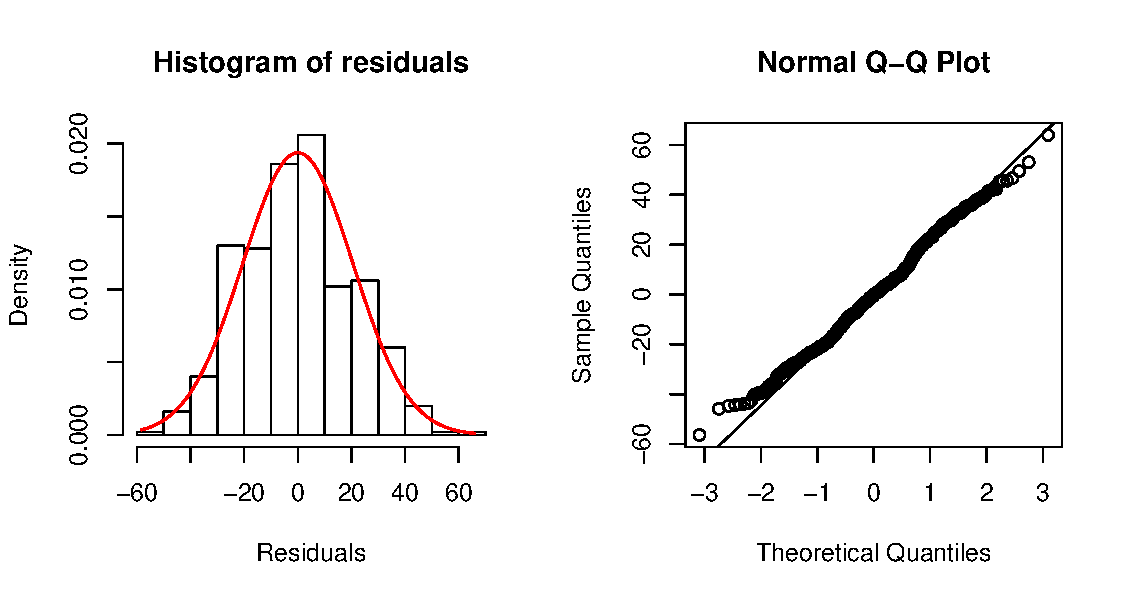
\includegraphics[width=\maxwidth]{figure/unnamed-chunk-118-1} 

}



\end{knitrout}

\section{Analysis of the FAMuSS Dataset}
Going back to the FAMuSS dataset, a more comprehensive study can now be performed using multiple linear regression to account for various confounders.  As a baseline, two different simple linear regressions can be computed as follows, the goal of the following analysis to be to improve upon this simple model.  

\begin{knitrout}
\definecolor{shadecolor}{rgb}{0.969, 0.969, 0.969}\color{fgcolor}\begin{kframe}
\begin{alltt}
\hlcom{## Simple genotype model - significant}
\hlkwd{summary}\hlstd{(}\hlkwd{lm}\hlstd{(}\hlkwd{log}\hlstd{(famuss}\hlopt{$}\hlstd{ndrm.ch}\hlopt{+}\hlnum{5}\hlstd{)} \hlopt{~} \hlstd{famuss}\hlopt{$}\hlstd{actn3.r577x))}
\end{alltt}
\begin{verbatim}
## 
## Call:
## lm(formula = log(famuss$ndrm.ch + 5) ~ famuss$actn3.r577x)
## 
## Residuals:
##      Min       1Q   Median       3Q      Max 
## -2.37691 -0.34090  0.02099  0.39878  1.64371 
## 
## Coefficients:
##                      Estimate Std. Error t value Pr(>|t|)    
## (Intercept)           3.81335    0.04722  80.763   <2e-16 ***
## famuss$actn3.r577xCT  0.08420    0.06089   1.383   0.1672    
## famuss$actn3.r577xTT  0.17300    0.06801   2.544   0.0112 *  
## ---
## Signif. codes:  0 '***' 0.001 '**' 0.01 '*' 0.05 '.' 0.1 ' ' 1
## 
## Residual standard error: 0.621 on 592 degrees of freedom
## Multiple R-squared:  0.01081,	Adjusted R-squared:  0.007471 
## F-statistic: 3.236 on 2 and 592 DF,  p-value: 0.04003
\end{verbatim}
\begin{alltt}
\hlcom{## Simple age model - significant }
\hlkwd{summary}\hlstd{(}\hlkwd{lm}\hlstd{(}\hlkwd{log}\hlstd{(famuss}\hlopt{$}\hlstd{ndrm.ch}\hlopt{+}\hlnum{5}\hlstd{)} \hlopt{~} \hlstd{famuss}\hlopt{$}\hlstd{age))}
\end{alltt}
\begin{verbatim}
## 
## Call:
## lm(formula = log(famuss$ndrm.ch + 5) ~ famuss$age)
## 
## Residuals:
##      Min       1Q   Median       3Q      Max 
## -2.40718 -0.32241  0.04502  0.39529  1.72844 
## 
## Coefficients:
##             Estimate Std. Error t value Pr(>|t|)    
## (Intercept)  4.55967    0.10685  42.675  < 2e-16 ***
## famuss$age  -0.02715    0.00426  -6.374 3.69e-10 ***
## ---
## Signif. codes:  0 '***' 0.001 '**' 0.01 '*' 0.05 '.' 0.1 ' ' 1
## 
## Residual standard error: 0.6036 on 593 degrees of freedom
## Multiple R-squared:  0.06413,	Adjusted R-squared:  0.06255 
## F-statistic: 40.63 on 1 and 593 DF,  p-value: 3.691e-10
\end{verbatim}
\begin{alltt}
\hlcom{## Simple bmi model -significant}
\hlkwd{summary}\hlstd{(}\hlkwd{lm}\hlstd{(}\hlkwd{log}\hlstd{(famuss}\hlopt{$}\hlstd{ndrm.ch}\hlopt{+}\hlnum{5}\hlstd{)} \hlopt{~} \hlstd{famuss}\hlopt{$}\hlstd{bmi))}
\end{alltt}
\begin{verbatim}
## 
## Call:
## lm(formula = log(famuss$ndrm.ch + 5) ~ famuss$bmi)
## 
## Residuals:
##      Min       1Q   Median       3Q      Max 
## -2.40374 -0.31402  0.04119  0.40282  1.57997 
## 
## Coefficients:
##              Estimate Std. Error t value Pr(>|t|)    
## (Intercept)  4.378313   0.137397  31.866  < 2e-16 ***
## famuss$bmi  -0.019721   0.005534  -3.563 0.000396 ***
## ---
## Signif. codes:  0 '***' 0.001 '**' 0.01 '*' 0.05 '.' 0.1 ' ' 1
## 
## Residual standard error: 0.6173 on 593 degrees of freedom
## Multiple R-squared:  0.02096,	Adjusted R-squared:  0.01931 
## F-statistic:  12.7 on 1 and 593 DF,  p-value: 0.0003956
\end{verbatim}
\begin{alltt}
\hlcom{## Simple sex model - significant}
\hlkwd{summary}\hlstd{(}\hlkwd{lm}\hlstd{(}\hlkwd{log}\hlstd{(famuss}\hlopt{$}\hlstd{ndrm.ch}\hlopt{+}\hlnum{5}\hlstd{)} \hlopt{~} \hlstd{famuss}\hlopt{$}\hlstd{sex))}
\end{alltt}
\begin{verbatim}
## 
## Call:
## lm(formula = log(famuss$ndrm.ch + 5) ~ famuss$sex)
## 
## Residuals:
##      Min       1Q   Median       3Q      Max 
## -2.44037 -0.30030  0.07516  0.39285  1.49146 
## 
## Coefficients:
##                Estimate Std. Error t value Pr(>|t|)    
## (Intercept)     4.04981    0.03172 127.685  < 2e-16 ***
## famuss$sexMale -0.37546    0.04973  -7.549 1.66e-13 ***
## ---
## Signif. codes:  0 '***' 0.001 '**' 0.01 '*' 0.05 '.' 0.1 ' ' 1
## 
## Residual standard error: 0.5959 on 593 degrees of freedom
## Multiple R-squared:  0.08768,	Adjusted R-squared:  0.08615 
## F-statistic: 56.99 on 1 and 593 DF,  p-value: 1.657e-13
\end{verbatim}
\begin{alltt}
\hlcom{## Simple race model - insignificant}
\hlkwd{summary}\hlstd{(}\hlkwd{lm}\hlstd{(}\hlkwd{log}\hlstd{(famuss}\hlopt{$}\hlstd{ndrm.ch}\hlopt{+}\hlnum{5}\hlstd{)} \hlopt{~} \hlstd{famuss}\hlopt{$}\hlstd{race))}
\end{alltt}
\begin{verbatim}
## 
## Call:
## lm(formula = log(famuss$ndrm.ch + 5) ~ famuss$race)
## 
## Residuals:
##      Min       1Q   Median       3Q      Max 
## -2.31523 -0.29080  0.08267  0.42740  1.61660 
## 
## Coefficients:
##                       Estimate Std. Error t value Pr(>|t|)    
## (Intercept)           3.926241   0.119685  32.805   <2e-16 ***
## famuss$raceAsian     -0.150366   0.146139  -1.029    0.304    
## famuss$raceCaucasian -0.001573   0.123096  -0.013    0.990    
## famuss$raceHispanic  -0.272195   0.176466  -1.542    0.123    
## famuss$raceOther     -0.090221   0.176466  -0.511    0.609    
## ---
## Signif. codes:  0 '***' 0.001 '**' 0.01 '*' 0.05 '.' 0.1 ' ' 1
## 
## Residual standard error: 0.6219 on 590 degrees of freedom
## Multiple R-squared:  0.0114,	Adjusted R-squared:  0.004694 
## F-statistic:   1.7 on 4 and 590 DF,  p-value: 0.1483
\end{verbatim}
\end{kframe}
\end{knitrout}

One question that may come up from the following line of code is why the gene actn3.577x, the sex, or the race are not coded as a factor in this regression line, and the simple answer is that the dataset already has these variables coded as a factor.  To test if this is the case or not, the function \textit{class()} can be used, which will tell the variable type.  

\begin{knitrout}
\definecolor{shadecolor}{rgb}{0.969, 0.969, 0.969}\color{fgcolor}\begin{kframe}
\begin{alltt}
\hlkwd{class}\hlstd{(famuss}\hlopt{$}\hlstd{actn3.r577x)}
\end{alltt}
\begin{verbatim}
## [1] "factor"
\end{verbatim}
\end{kframe}
\end{knitrout}

Now, using the information based on the single regressions, a multiple regression can be built.  Both the residuals and the $R^2$ indicate that this model is far from great.  The main text talks through why this inaccuracy could be caused by data collection error and is unlikely to be an indication of fallacy in the methods.  
\begin{knitrout}
\definecolor{shadecolor}{rgb}{0.969, 0.969, 0.969}\color{fgcolor}\begin{kframe}
\begin{alltt}
\hlkwd{summary}\hlstd{(}\hlkwd{lm}\hlstd{(}\hlkwd{log}\hlstd{(famuss}\hlopt{$}\hlstd{ndrm.ch} \hlopt{+} \hlnum{5}\hlstd{)} \hlopt{~} \hlstd{famuss}\hlopt{$}\hlstd{actn3.r577x} \hlopt{+} \hlstd{famuss}\hlopt{$}\hlstd{age} \hlopt{+} \hlstd{famuss}\hlopt{$}\hlstd{sex} \hlopt{+}
    \hlstd{famuss}\hlopt{$}\hlstd{bmi))}
\end{alltt}
\begin{verbatim}
## 
## Call:
## lm(formula = log(famuss$ndrm.ch + 5) ~ famuss$actn3.r577x + famuss$age + 
##     famuss$sex + famuss$bmi)
## 
## Residuals:
##      Min       1Q   Median       3Q      Max 
## -2.56248 -0.28173  0.04579  0.39561  1.49186 
## 
## Coefficients:
##                       Estimate Std. Error t value Pr(>|t|)    
## (Intercept)           4.763789   0.156155  30.507  < 2e-16 ***
## famuss$actn3.r577xCT  0.067869   0.056746   1.196   0.2322    
## famuss$actn3.r577xTT  0.139577   0.063286   2.205   0.0278 *  
## famuss$age           -0.023044   0.004169  -5.527 4.90e-08 ***
## famuss$sexMale       -0.348692   0.048436  -7.199 1.86e-12 ***
## famuss$bmi           -0.009430   0.005292  -1.782   0.0753 .  
## ---
## Signif. codes:  0 '***' 0.001 '**' 0.01 '*' 0.05 '.' 0.1 ' ' 1
## 
## Residual standard error: 0.5756 on 589 degrees of freedom
## Multiple R-squared:  0.1546,	Adjusted R-squared:  0.1474 
## F-statistic: 21.54 on 5 and 589 DF,  p-value: < 2.2e-16
\end{verbatim}
\begin{alltt}
\hlstd{residuals} \hlkwb{=} \hlkwd{resid}\hlstd{(}\hlkwd{lm}\hlstd{(}\hlkwd{log}\hlstd{(famuss}\hlopt{$}\hlstd{ndrm.ch} \hlopt{+} \hlnum{5}\hlstd{)} \hlopt{~} \hlstd{famuss}\hlopt{$}\hlstd{actn3.r577x} \hlopt{+} \hlstd{famuss}\hlopt{$}\hlstd{age} \hlopt{+}
    \hlstd{famuss}\hlopt{$}\hlstd{sex} \hlopt{+} \hlstd{famuss}\hlopt{$}\hlstd{bmi))}
\hlkwd{par}\hlstd{(}\hlkwc{mfrow} \hlstd{=} \hlkwd{c}\hlstd{(}\hlnum{1}\hlstd{,} \hlnum{2}\hlstd{))}
\hlkwd{hist}\hlstd{(residuals,} \hlkwc{xlab} \hlstd{=} \hlstr{"Residuals"}\hlstd{,} \hlkwc{freq} \hlstd{=} \hlnum{FALSE}\hlstd{)}
\hlstd{x} \hlkwb{<-} \hlkwd{seq}\hlstd{(}\hlkwd{min}\hlstd{(residuals)} \hlopt{-} \hlnum{2}\hlstd{,} \hlkwd{max}\hlstd{(residuals)} \hlopt{+} \hlnum{2}\hlstd{,} \hlnum{0.01}\hlstd{)}
\hlstd{y} \hlkwb{<-} \hlkwd{dnorm}\hlstd{(x,} \hlkwd{mean}\hlstd{(residuals),} \hlkwd{sd}\hlstd{(residuals))}
\hlkwd{lines}\hlstd{(x, y,} \hlkwc{lwd} \hlstd{=} \hlnum{1.5}\hlstd{,} \hlkwc{col} \hlstd{=} \hlstr{"red"}\hlstd{)}

\hlkwd{qqnorm}\hlstd{(residuals)}
\hlkwd{qqline}\hlstd{(residuals)}
\end{alltt}
\end{kframe}

{\centering 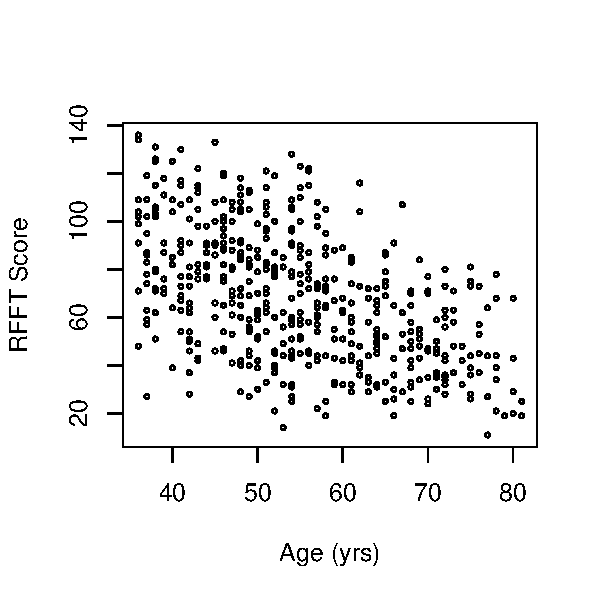
\includegraphics[width=\maxwidth]{figure/unnamed-chunk-121-1} 

}



\end{knitrout}



\end{document}
